\documentclass[12pt, twoside]{report}
	\usepackage[margin=1in]{geometry}
	\usepackage[hidelinks, linktoc=all, pagebackref, russian]{hyperref}
	\usepackage{indentfirst}
	\usepackage{latexsym}
    \usepackage[russian]{babel}
    \usepackage{subcaption}
    \captionsetup[subfigure]{justification=centering}
    \usepackage{wrapfig}
   	\usepackage[superscript,biblabel]{cite}
    \usepackage[font=small,labelfont=bf, justification=centering]{caption}
    \usepackage{abstract}
    \usepackage{mathtools}
    \usepackage{fancyhdr}
    \usepackage{bbm}
    \usepackage{bm}
    \usepackage{cleveref}
    \setlength{\parskip}{0.1cm}   
	\setlength{\parindent}{0.7cm}
    \usepackage{graphicx} % Used to insert images
    \usepackage{adjustbox} % Used to constrain images to a maximum size 
   	\usepackage{color} % Allow colors to be defined
    \usepackage{enumerate} % Needed for markdown enumerations to work
    \usepackage{geometry} % Used to adjust the document margins
    \usepackage{amsmath} % Equations
    \usepackage{amssymb} % Equations
    \usepackage[mathletters]{ucs} % Extended unicode (utf-8) support
    \usepackage[utf8x]{inputenc} % Allow utf-8 characters in the tex document
    \usepackage{fancyvrb} % verbatim replacement that allows latex
    \usepackage{grffile} % extends the file name processing of package graphics 
                         % to support a larger range 
    % The hyperref package gives us a pdf with properly built
    % internal navigation ('pdf bookmarks' for the table of contents,
    % internal cross-reference links, web links for URLs, etc.)
    \usepackage{longtable} % longtable support required by pandoc >1.10
	%\usepackage{physics}

 	
\addto\extrasrussian{%
  \renewcommand{\figureautorefname}{Рис.}%
}
\newcommand{\Tr}[1]{\text{Tr}\left[#1\right]}
\newcommand{\pTr}[2]{\text{Tr}_{#1}\left[#2\right]}

\DeclarePairedDelimiter\bra{\langle}{\rvert}
\DeclarePairedDelimiter\ket{\lvert}{\rangle}
\DeclarePairedDelimiterX\braket[2]{\langle}{\rangle}{#1 \delimsize\vert #2}
\newcommand{\rbrkt}[1]{\left( #1 \right)}
\newcommand{\sbrkt}[1]{\left[ #1 \right]}
\renewcommand*{\backreftwosep}{ и~}
\renewcommand*{\backreflastsep}{ и~}
\renewcommand*{\backref}[1]{}
\renewcommand*{\backrefalt}[4]{%
\ifcase #1 %
\relax%
\or
(ссылка на стр. [#2])%
\else
(ссылки на стр. [#2])%
\fi
}

\numberwithin{equation}{section}
\numberwithin{figure}{section}

\renewcommand*\thesection{\arabic{section}}
\lhead[\rm\thepage]{\fancyplain{}{\nouppercase{\sl{\rightmark}}}}
\rhead[\fancyplain{}{\nouppercase{\sl{\leftmark}}}]{\rm\thepage}
\chead{}\lfoot{}\rfoot{}\cfoot{}
\pagestyle{fancy}


\begin{document}
\newif\ifdraft
\drafttrue

\ifdraft

\begin{titlepage}
\begin{center}
Государственное образовательное учреждение высшего профессионального образования\\
Московский Физико-Технический Институт (Государственный Университет)\\
Факультет общей и прикладной физики\\
Кафедра физики и технологии наноструктур\\
\end{center}

\vspace{5cm}

\begin{center}

Выпускная квалификационная работа бакалавра\\~\\
\Large \textbf{Оптимизация однокубитных и двухкубитных вентилей и считывающих импульсов для сверхпроводниковых кубитов}
\end{center}

\vspace{4cm}
\begin{center}
\begin{minipage}{0.45\textwidth}
\begin{center}
Выполнил студент:\\~\\~\\
Сафронов Е.С.\\
группа 325
\end{center}
\end{minipage}
\begin{minipage}{0.45\textwidth}
\begin{center}
Научный руководитель:\\~\\~\\
Шульга К.В.\\
к. ф.-м. н.
\end{center}
\end{minipage}
\end{center}

\vspace{\fill}

\begin{center}
г. Москва, 2017
\end{center}
\end{titlepage}

\newgeometry{right=1in, left = 1.2in, top=1in, bottom=1in}

\tableofcontents
\newpage

\chapter{Введение}
Квантовый компьютер -- это устройство, хранящее и обрабатывающее информацию внутри группы квантовых систем, причем обработка информации происходит в результате когерентных взаимодействий систем внутри группы \cite{Lloyd1993}. Каждая квантовая система, как правило, является двухуровневой и носит название ``квантовый бит'' или ``кубит'' (англ. ``qubit'' -- quantum bit). Для осуществления квантового расчета необходимо связать кубиты друг с другом, иметь возможность управлять состоянием кубитов и считывать его, сохраняя чистоту соответствующей матрицы плотности, а также обеспечить изоляцию кубитов от влияния окружающей среды. Следовательно, в качестве кубитов могут быть использованы любые достаточно изолированные двухуровневые системы, поддающиеся контролю и способные взаимодействовать друг с другом \cite{DiVincenzo1995, DiVincenzo2000, Spiller1996}. В качестве примера можно привести фотоны \cite{Milburn2009}, ионы в ионных ловушках \cite{Cirac1995}, ядерные спины \cite{Kane1998}, атомы в электромагнитных резонаторах\cite{Rempe2008},  электрические системы\cite{Devoret2005} и т.п.

Последние являются одними их самых заманчивых кандидатов на эту роль, но только при условии, что их поведение будет именно квантовым, а не классическим\cite{Devoret1995}. К счастью, явление сверхпроводимости и эффект Джозефсона позволяют наблюдать квантовые эффекты в контурах даже мезоскопического масштаба и создавать на их основе так называемые \textit{сверхпроводящие (джозефсоновские) кубиты}\cite{Clarke2008}. 
\iffalse 
В данной работе проводится исследование одного из них -- потокового сверхпроводящего кубита (Flux-кубит, впервые предложен в статье T. Orlando et al.\cite{Orlando1999}).
\fi

Джозефсоновские кубиты имеют два значительных недостатка и одно значительное преимущество в сравнении с микроскопическими кубитами. Первый недостаток заключается в значительном взаимодействии с окружающей средой - в силу больших размеров, джозефсоновские кубиты сильнее связываются со средой, что требует дополнительных изысканий в области их изоляции; второй недостаток заключается в том, что в то время как микроскопические кубиты, например, атомы, идентичны друг другу, сверхпроводящие кубиты могут иметь отличия из-за неточностей производства. Для борьбы с этим требуется либо создавать заведомо нечувствительные к дефектам схемы, либо проводить калибровку, в процессе которой параметры цепей измеряются, а затем компенсируются в эксперименте.

Преимущество джозефсоновских кубитов в их гибкости: они могут быть произвольным образом расположены относительно друг друга, а их параметры легко и непрерывно изменяемы в широких пределах. Эта гибкость вместе с некоторыми фундаментальными эффектами\cite{Koch2007} может быть использована для борьбы с первым недостатком, а также предоставляет много вариантов для подстройки параметров, что в значительной степени нивелирует второй недостаток. Далее, накопленный опыт человечества в области изготовления интегральных схем позволит упростить переход к производству реальных квантовых вычислительных устройств, что является еще одним преимуществом в сравнении с другими типами кубитов. Таким образом, скорее всего именно джозефсоновские кубиты и будут применены в первом квантовом компьютере, и именно их следует изучать.

Важно отметить, что сверхпроводящие кубиты могут применяться не только для непосредственного использования в квантовом компьютере, так как по сути являются рукотворными атомами с широко изменяемыми характеристиками, как внутренними, так и касающимися связи с окружением. Они могут быть пригодны для создания метаматериалов \cite{Macha2014}, проведения высокоточных измерений полей\cite{Clarke2006}, использоваться в качестве активной среды\cite{Astafiev2010}, применяться в квантовой криптографии и телепортации \cite{Xia2014} и т. п. 
\newpage



\chapter{Теоретические сведения} \label{chap:theory}
В этой главе приведены теоретическое описание некоторых явлений, учитываемых при построении модели сверхпроводящих кубитов. Далее будет кратко рассмотрен эффект Джозефсона, затем произведено рассмотрение теории изолированного сверхпроводящего кубита и его частного случая -- \textit{трансмона}, теории его взаимодействия с окружающей средой и, наконец, вопросы измерения и контроля. 

\iffalse
\section{Явление сверхпроводимости}
Сверхпроводимость -- это сложное коллективное явление, свойство некоторых материалов обладать строго нулевым электрическим сопротивлением при достижении ими температуры ниже определенного значения. В настоящий момент самой известной точной теорией сверхпроводимости является теория БКШ\cite{Schrieffer1999}, согласно которой электроны в сверхпроводнике при переходе через критическую температуру объединяются в так называемые куперовские пары и претерпевают бозе-конденсацию. Спаривание электронов происходит в результате обмена фононами, приводящего к эффективному притяжению между ними и образованию связанного состояния на уровне Ферми, отделенного от уровней квазичастичных возбуждений энергетической щелью. Полное описание данного эффекта в рамках микроскопической теории невозможно в данной работе, поэтому мы будем далее пользоваться феноменологической теорией Гинзбурга-Ландау \cite{GL1950}, которая выводится из модели БКШ\cite{Gorkov1959}, но является более удобной в практическом применении. Сверхпроводящее состояние в рамках этой теории может быть описано параметром порядка или, иначе, модулем так называемой "макроскопической волновой функции куперовских пар":
\begin{equation}
\Psi(\mathbf{r}) = \sqrt{\frac{n_s}{2}}e^{i\theta(\mathbf{r})},
\label{eq:glwf} 
\end{equation}
где $n_s$ -- концентрация сверхпроводящих электронов в сверхпроводнике. Важно подчеркнуть, что она не является настоящей волновой функцией, но тем не менее позволяет получить практически важные результаты. Мы далее считаем, что в изолированном невозмущенном полями сверхпроводнике и модуль, и фаза волновой функции (\ref{eq:glwf}) постоянны.

Из минимизации функционала Гинзбурга-Ландау и одного из уравнений Максвелла можно получить следующее уравнение для сверхпроводящего тока куперовских пар в зависимости от приложенного поля, являющееся обобщением уравнения Лондонов:
\begin{equation}
\mathbf{j}_s = -\frac{i\hbar e}{2m_e}(\Psi^*\nabla\Psi - \Psi\nabla\Psi^*) - \frac{2e^2}{m_e}\mathbf{A}|\Psi|^2.
\label{eq:lond}
\end{equation}
Подставляя сюда $\Psi(\mathbf{r})$ из определения (\ref{eq:glwf}), получим:
\begin{equation}
\mathbf{j}_s = \frac{1}{\Lambda}\left(\frac{\Phi_0}{2\pi}\nabla\theta(\mathbf{r})-\mathbf{A}\right),
\label{eq:lond2}
\end{equation}
где $\displaystyle \Lambda = \frac{m_e}{n_s e^2},\ \Phi_0 = \frac{h}{2e}$. Вторая константа, как будет показано далее, является \textit{квантом магнитного потока}, и имеет важное значение в данной работе.
\fi


\section{Эффект Джозефсона}
\subsection{Уравнения Джозефсона}
Эффект Джозефсона\cite{Josephson1964} -- это макроскопических квантовый эффект в сверхпроводниках. Согласно теории БКШ, сверпроводящее состояние проводника может быть описано параметром порядка, являющимся модулем макроскопической волновой функции куперовских пар:
\begin{equation}
\Psi(\mathbf{r}) = \sqrt{\frac{n_s}{2}}e^{i\theta(\mathbf{r})},
\label{eq:glwf} 
\end{equation}
\textit{Тогда}, эффект Джозефсона заключается в установления одной фазы в двух сверхпроводниках, соединенных через ``слабую связь''. ``Слабые связи'' многообразны: это могут быть тонкие слои диэлектрика, сужения, точечные контакты, прослойки из металла в нормальном состоянии или из ферромагнетика. В случае, если фазы не равны, то через слабую связь будет течь бездиссипативный ток, и будет выполнено некоторое \textit{фазо-токовое соотношение} между током и скачком фазы на переходе. Часто, хотя и не всегда\cite{Golubov2004}, оно оказывается синусоидальным:
\begin{equation}
I_s = I_c \sin(\theta_2 - \theta_1) = I_c \sin\varphi.
\label{eq:CPR}
\end{equation}
Из этой формулы видно, что сверхпроводящий ток $I_s$ не может превысить некоторого значения $I_c$. Это так называемый \textit{критический ток} джозефсоновского перехода, при превышении которого бездиссипативность нарушается, и на переходе устанавливается напряжение V. В этом случае выполнено второе уравнение Джозефсона:
\begin{equation}
\hbar \frac{\partial \varphi}{\partial t} = 2eV,
\label{eq:2JE}
\end{equation}
и наблюдаются осцилляции разности фаз между сверхпроводниками. Величина критического тока рассчитывается из микроскопической теории, например, для перехода SIS (\textit{сверхпроводник - изолятор - сверхпроводник}) верна формула Амбегаокара-Баратова:
\begin{equation}
I_c = \frac{\pi\Delta(T)}{2eR_n}\th\left(\frac{\Delta(T)}{2k_bT}\right),
\label{eq:Ic}
\end{equation}
где через $T$ обозначена температура, а через $R_n$ сопротивление контакта в отсутствие сверхпроводимости, $R_n = \rho\frac{d}{S}$, где $\rho$ -- удельное сопротивление I-слоя, а $d$ и $S$ -- его толщина и площадь.
\subsection{RCSJ-модель}
Для упрощения описания динамики джозефсоновского контакта применяется модель RCSJ (Resistively and Capacitively Shunted Junction), работающая для маленьких переходов со слоем изолятора, когда изменения фазы на размере контакта пренебрежимо малы и присутствует ненулевая геометрическая емкость. 
\begin{figure}[h]
\centering
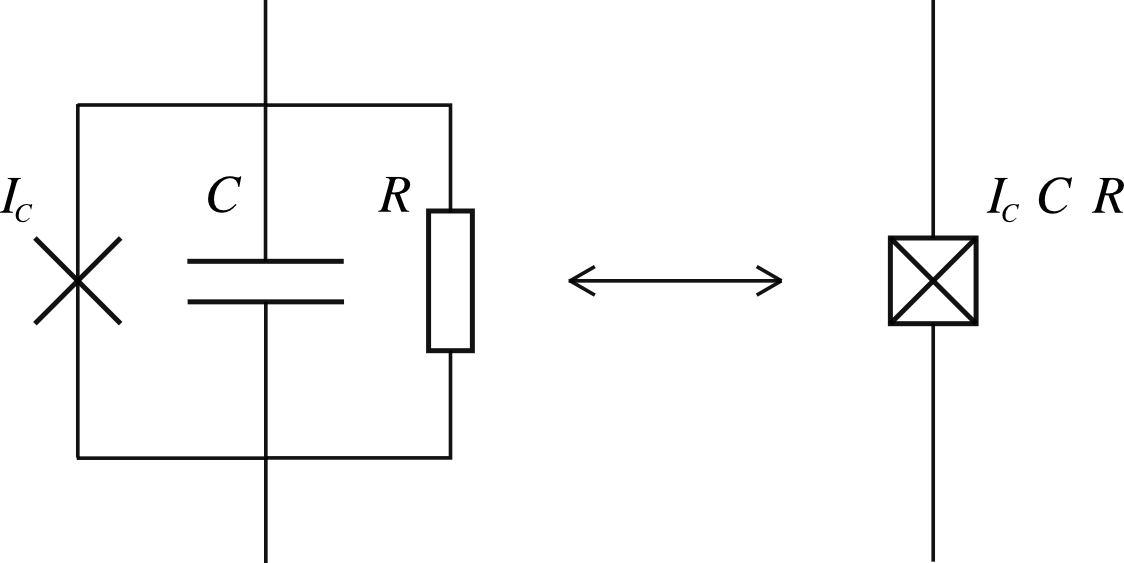
\includegraphics[width=0.65\textwidth]{Pictures/RCSJ.png}
\caption{Схема RCSJ в виде параллельного соединения идеального джозефсоновского перехода с конденсатором и резистором.}
\label{fig:RSCJ}
\end{figure}

Принципиальная схема изображена на \autoref{fig:RSCJ}. В случае, когда ток через систему не превышает критического $I_c$, резистор на схеме может быть опущен. В силу параллельности соединения выполнено также соотношение $\frac{\hbar}{2e}\frac{\partial\varphi}{\partial t} = U_C$ между напряжениями на переходе и на конденсаторе, которое устанавливает аналогию между неидеальным переходом и колебательным контуром с нелинейной индуктивностью.

В рамках RCSJ-модели энергия перехода состоит из энергии, запасенной в нелинейной индуктивности идеального перехода, и энергии конденсатора:
\begin{equation}
E = E_{ind}+E_{cap}  \label{eq:JJenrj1}
\end{equation}

Индуктивная энергия может быть определена посредством интегрирования мощности $P = IV$ по времени от 0 до момента Т, когда на контакте установилась разность фаз $\varphi$:
\begin{equation}
\begin{gathered}
E_{ind} = \int I_JV_J\, dt = I_c \frac{\hbar}{2e}\int_0^T \sin(\phi(t))\frac{d\phi(t)}{dt}dt  \\ 
= E_J \int_0^\varphi \sin\phi\, d\phi = E_J [1-\cos\varphi],
\end{gathered}
\end{equation}
где была введена новая константа $E_J$ -- джозефсоновская энергия. Емкостная энергия также может быть вычислена с использованием \eqref{eq:2JE}:
\begin{equation}
E_{cap} = \frac{1}{2}C U_C^2 = \frac{1}{2} C \left(\frac{\Phi_0}{2\pi}\right)^2 \dot \varphi^2 = 
\frac{\hbar^2}{E_C} \dot \varphi^2,\ E_C = \frac{(e)^2}{2C},
\label{eq:JJenrj2}
\end{equation}
где $E_C$ -- константа, описывающая емкостную энергию перехода.

\subsection{Фазо-потоковое соотношение}
Рассмотрим замкнутое сверхпроводящее кольцо конечной толщины, быть может, прерванное конечным числом джозефсоновских переходов $\{J_1..J_n\}$. Рассмотрим применительно к данному случаю уравнение (\ref{eq:lond2}). Проведем контур $C$ внутри кольца так, чтобы он нигде не приближался к стенкам на расстояние, меньшее глубины проникновения магнитного поля (\autoref{fig:ring}). Тогда сверхток на всей его длине будет равен нулю, и, проинтегрировав по нему (\ref{eq:lond2}), мы получим следующее равенство:
\begin{equation}
\oint\displaylimits_C \mathbf{A}d\mathbf{l} = \frac{\Phi_0}{2\pi}\oint\displaylimits_C \nabla \theta d \mathbf{l} \notag.
\end{equation}
Руководствуясь \autoref{fig:ring}, соображениями однозначности волновой функции (\ref{eq:glwf}) при обходе вокруг контура и теоремой Стокса для $\operatorname{rot} \mathbf{A}$, можем написать:
\begin{gather}
\Phi = \frac{\Phi_0}{2\pi}\left(\sum_i \varphi_i + 2\pi k\right) \Rightarrow \notag\\
\Rightarrow \sum_i \varphi_i = 2\pi\left(\frac{\Phi}{\Phi_0} - k\right),\ k\in \mathcal{Z}.
\label{eq:phsflx}
\end{gather}

\begin{figure}[h]
\centering
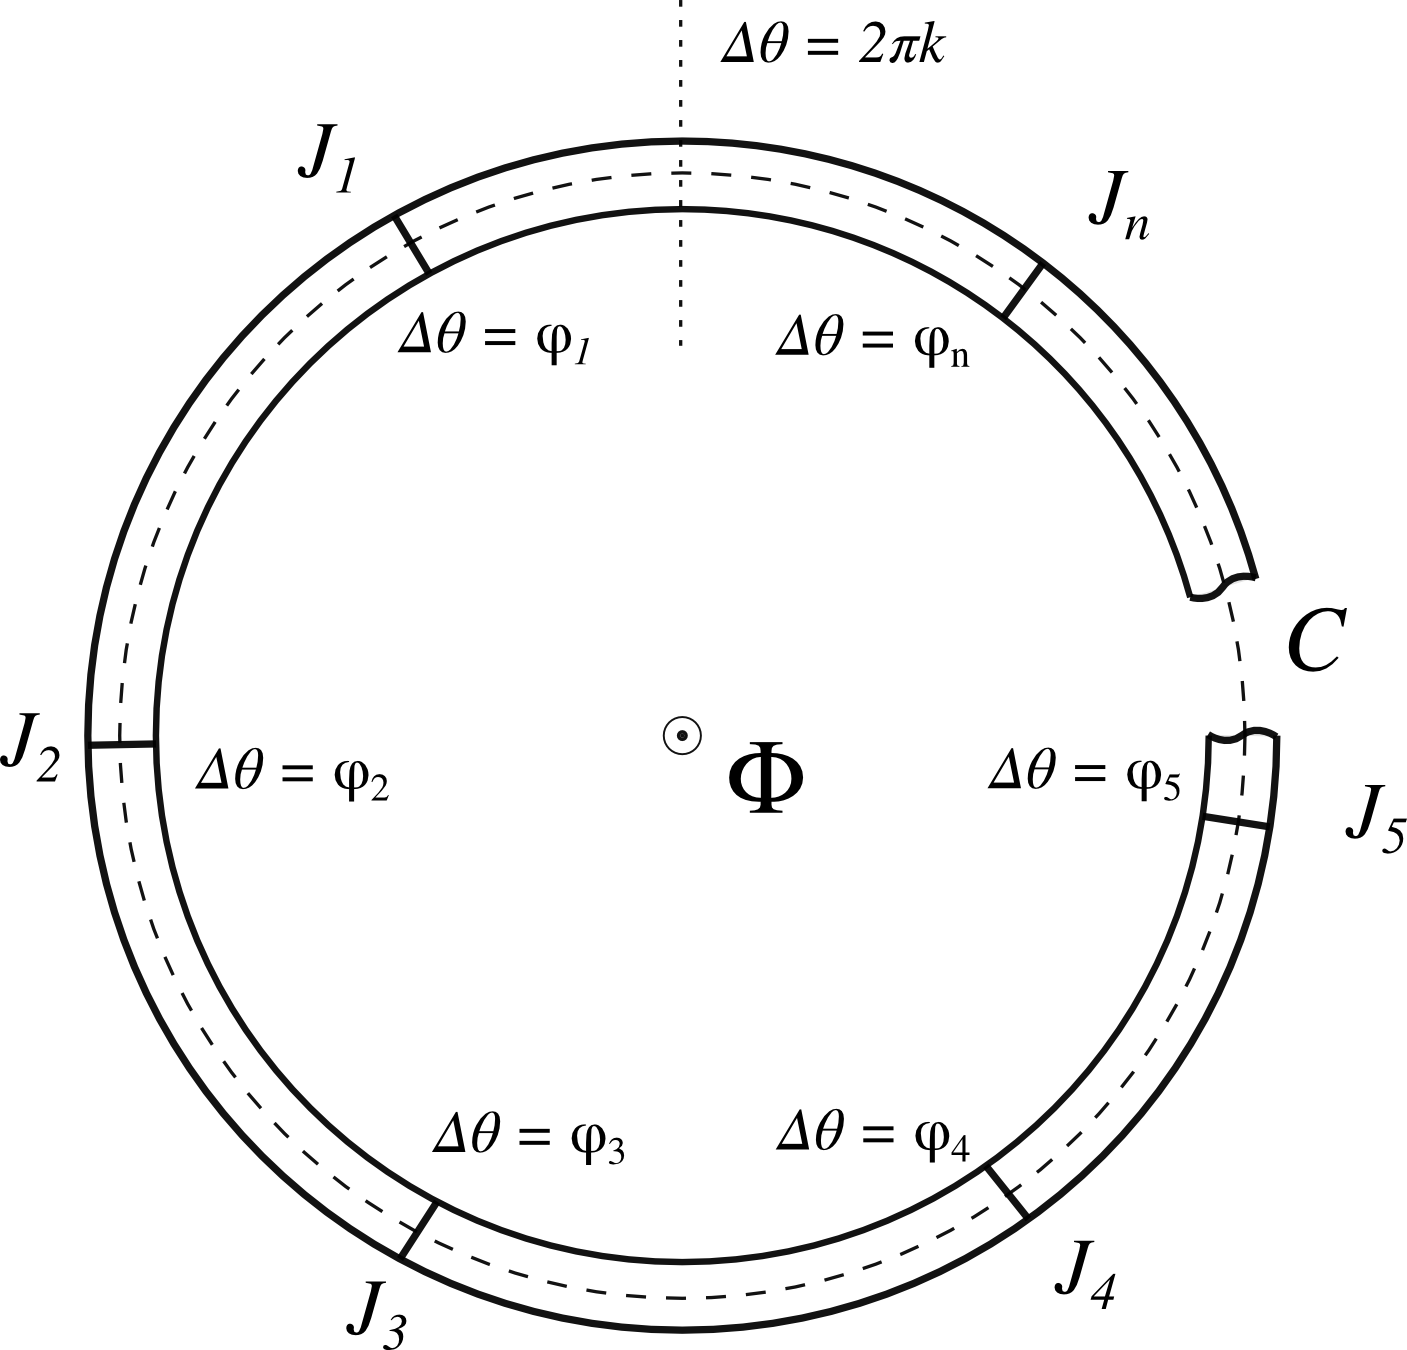
\includegraphics[width=0.5\linewidth]{Pictures/ring.png}
\caption{К выводу фазо-потокового соотношения. Пунктиром обозначен контур интегрирования $C$. Через $\varphi_i$ обозначены скачки фаз на джозефсоновских контактах, а точками - место разрешенного накопления фазы при полном обходе вокруг кольца $2\pi k,\ k\in\mathcal{Z}$.}
\label{fig:ring}
\end{figure}

Таким образом, получено фазо-потоковое соотношение. Видно, что в случае отсутствия в кольце джозефсоновских переходов полученное уравнение (\ref{eq:phsflx}) опишет равенство магнитного потока $\Phi$, проходящего через сверхпроводящее кольцо, целому числу  k квантов потока $\Phi_0$, обосновывая определение этой константы в (\ref{eq:lond2}).


\section{Теория изолированного сверхпроводящего кубита}
Сверхпроводящие кубиты были предложен Леггеттом в 1980х, а в 1997м Yasunobu Nakamura году был проведен первый эксперимент, доказавший наличие суперпозиции состояний в сверхпроводящем кубите. Он исследовал состояния в ``ящике куперовских пар'' (англ. -- "Cooper-pair box") или иначе, \textit{зарядовом кубите}. В 1999 году был предложен Flux-кубит, или потоковый трехконтактный сверхпроводящий кубит \cite{Orlando1999}. Он представляет собой сверхпроводящий контур, прерванный в трех местах джозефсоновскими переходами (\autoref{fig:qubit}), два из которых одинаковы, а третий отличается по площади в $\alpha$ раз. Наконец, в 2007году был предложен \cite{Koch2007} \textit{трансмон} - схожий с зарядовым кубит, однако, с существенно подавленными зарядовыми шумами и несколько меньшим \textit{ангармонизмом}. 
Под \textit{изолированным} в данном разделе понимается одиночный кубит, не взаимодействующий с окружением ни диссипативным, ни консервативным образом. Единственным внешним фактором является при таком рассмотрении постоянное магнитное поле, проходящее через контур.

\subsection{Построение гамильтониана}
Для того, чтобы провести квантово-механическое рассмотрение кубита, требуется записать его гамильтониан. Для этого прежде всего нужно понять, какими независимыми степенями свободы он обладает. Вообще говоря, состояние одиночного джозефсоновского перехода, в силу того, что в параллельном соединении RCSJ-модели $U = \frac{\hbar}{2e}\dot\varphi$, целиком описывается своей разностью фаз. Энергия, запасенная шунтирующим конденсатором, может быть записана в виде (\ref{eq:JJenrj2}), а энергия джозефсоновского контакта в виде (\ref{eq:JJenrj1}). Таким образом, получаем гамильтониан системы:
\begin{equation}
\hat{H} = E_J \left[ 1 - cos\hat{\varphi} \right] + \frac{ \hbar^2 }{  E_C } \dot{\hat{\varphi}}^2
\label{eq:ham-qubit}
\end{equation}
Аналогично сопряженной паре операторов $\hat{x}$ и $\hat{p} = -i\hbar\frac{\partial}{\partial x }$ можно определить оператор заряда $\hat{q} = -2e i  \frac{\partial}{\partial \varphi }$ и числа куперовских пар $\hat{n} = - i \frac{\partial}{\partial \varphi }$. Кроме того, иногда заряд кубита можно контролировать посредством емкостного гейта $C_g$ с приложенным напряжением $V_g$. Тогда энергия, запасенная в емкостной части контура может быть записана как $4 E_C (\hat{n} - n_g )^2 $, где $n_g = {-C_g V_g \over 2e}$. Весь гамильтониан:
\begin{equation}
\hat{H} = 4 E_C (\hat{n} - n_g )^2 + E_J \left[1 - cos\hat{\varphi}\right]
\label{eq:ham-qubit-ng}
\end{equation}
Уровни энергии такого гамильтониана можно найти аналитически:
\begin{equation}
E_m(n_g) = E_C a_{2 \left[n_g+k\left(m,ng\right)\right]} (-\frac{E_J}{2 E_C})
\label{eq:ham-qubit-ng-anal}
\end{equation},
где $a_\nu(q)$ - функция Матьё, а $k(m,n_g)$ - целочисленная функция, задающая порядок собственных уровней энергии. Однако, для проведения численных расчетов решение в таком виде не является удобным. Рассмотрим гамильтониан \ref{eq:ham-qubit-ng} в зарядовом базисе (базисе собственных состояниях $\hat{n}$) :
\begin{equation}
\hat{H} = 4 E_C \left(\hat{n} - n_g\right)^2  - E_J \sum_{n = -\infty}^{\infty}
\left( 
\left|n+1 \right>\left<n   \right| +
\left|n   \right>\left<n+1 \right|
\right)
\label{eq:ham-qubit-charge-basis}
\end{equation}

Приблизим этот оператор конечноразмерным, отбросив состояния с зарядом, большим $2 e N$ по модулю: 
\begin{equation}
\hat{H}_N = 4 E_C \sum_{n = -N}^{N}\left(n - n_g\right)^2 \left| n \right>\left< n \right|  -
E_J \sum_{n = -N}^{N}
\left( 
\left| n+1 \right>\left< n   \right| +
\left| n   \right>\left< n+1 \right|
\right)
\label{eq:ham-qubit-charge-basis-N}
\end{equation}
Такой гамильтониан очень удобен для каких-либо численных расчетов. 

\subsection{Зарядовый кубит}
Зарядовый кубит представляет собой ящик для куперовских пар, связанных джозефсоновским контактом с резервуаром заряда и контролируемый приложенным напряжением на гейте. Электростатическая энергия системы...
\begin{equation}
E_C = C_J \frac{V^2}{2} + C_g \frac{\left(V_g-V\right)^2}{2} 
\end{equation}
\begin{equation}
E_C = \frac{C} { 2 } \left(V - \frac{C_g}{C} V_g\right)^2, C = C_J + C_g
\end{equation}
Сводится к привычному члену гамильтониана (\ref{eq:ham-qubit-ng}).
\newline
У зарядового кубита $E_J < E_C$. 
Популярный режим работы зарядового кубита - установка полуцелого заряда на островке ($n_g = 1/2$) с помощью управляющего напряжения (см рис. \ref{fig:charge-eigens-ng-2} и \ref{fig:charge-eigenstates}). Преимущество такого режима заключается в том, что эта точка расщепления уровней дает двухуровневую систему с разницей энергии уровней, равной $E_j$. Так же в этой точке наименьшая чувствительность к зарядовому шуму [ссылка].

%\newline
\begin{figure}[!h]
\begingroup
\captionsetup[subfigure]{width=0.9\textwidth, justification=normal}
\centering
\begin{subfigure}[t]{0.49\linewidth}
\centering
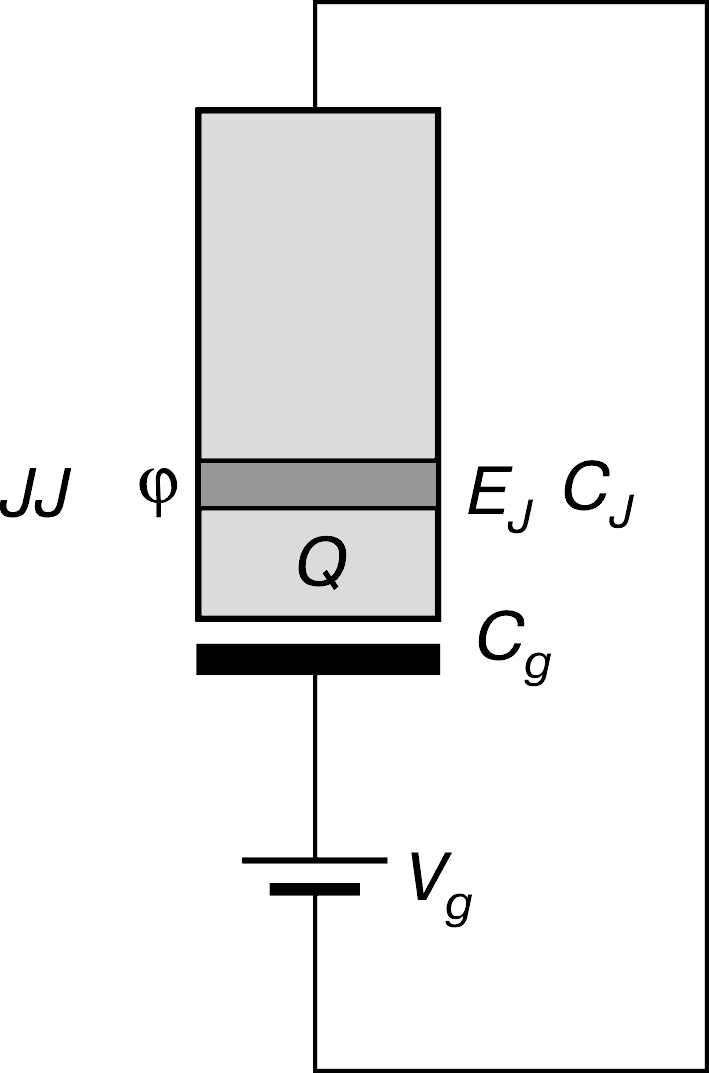
\includegraphics[height = .6\textwidth]{Pictures2/charge_qubit_scheme}
\caption{Схема зарядового кубита}
\label{fig:charge-scheme}
\end{subfigure}~
\begin{subfigure}[t]{0.49\linewidth}
\centering
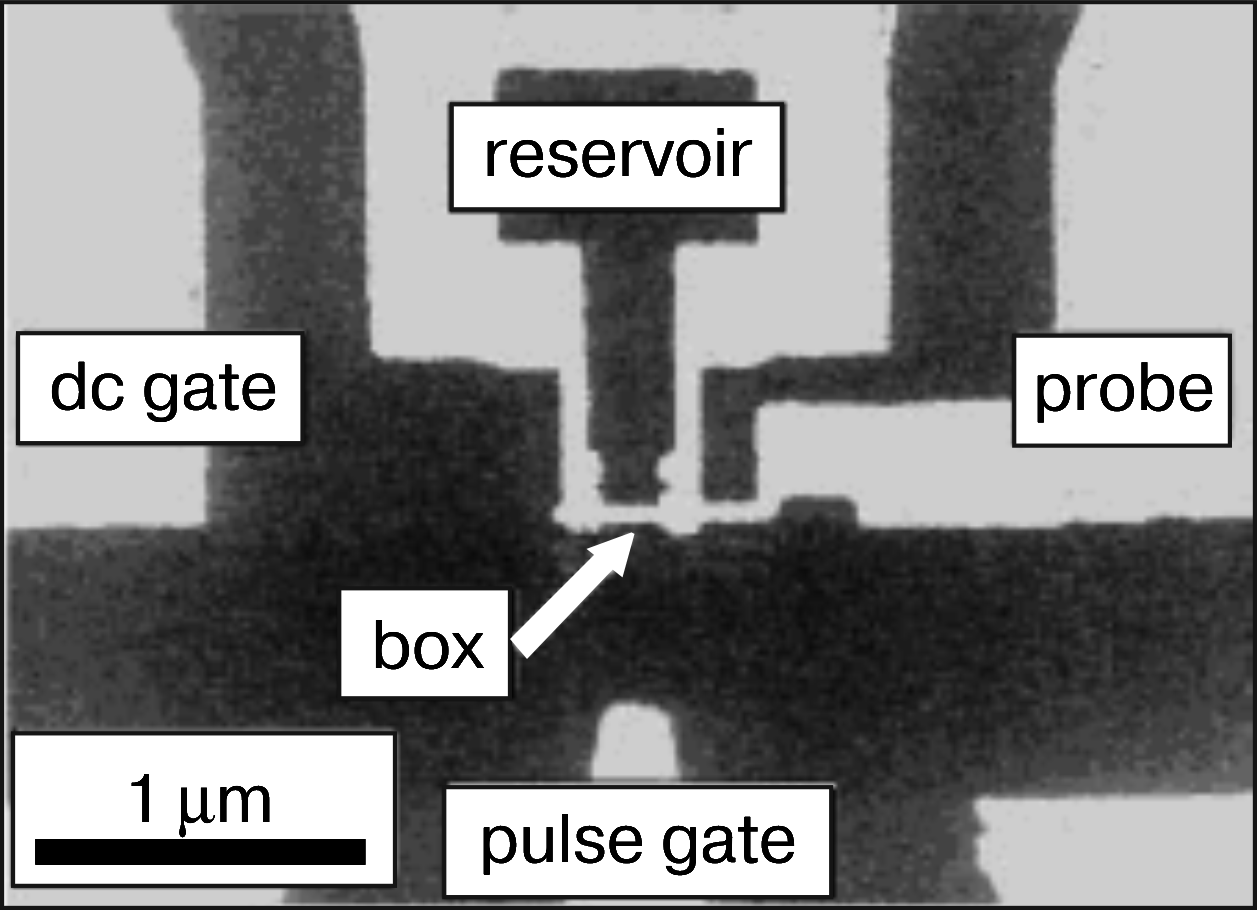
\includegraphics[height = .6\textwidth]{Pictures2/charge_qubit_photo}
\caption{Электронная фотография зарядового кубита [ссылка]}
\label{fig:charge-photo}
\end{subfigure}

\endgroup
\caption{}
\end{figure}

\begin{figure}[!h]
\begingroup
\captionsetup[subfigure]{width=0.9\textwidth, justification=normal}
\centering
\begin{subfigure}[t]{0.49\linewidth}
\centering
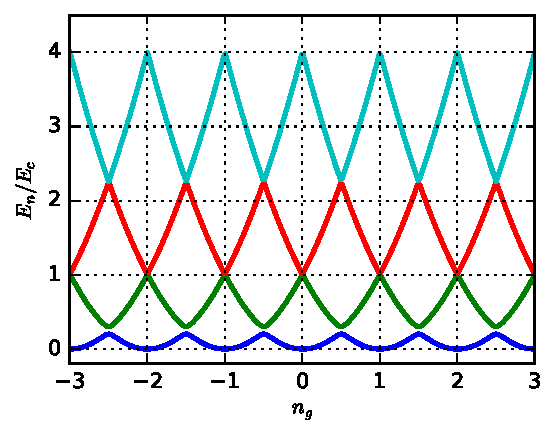
\includegraphics[height = .7\textwidth]{Pictures2/charge_qubit_01}
\caption{$E_C / E_J = 10$}
\label{fig:charge-eigens-ng-1}
\end{subfigure}~
\begin{subfigure}[t]{0.49\linewidth}
\centering
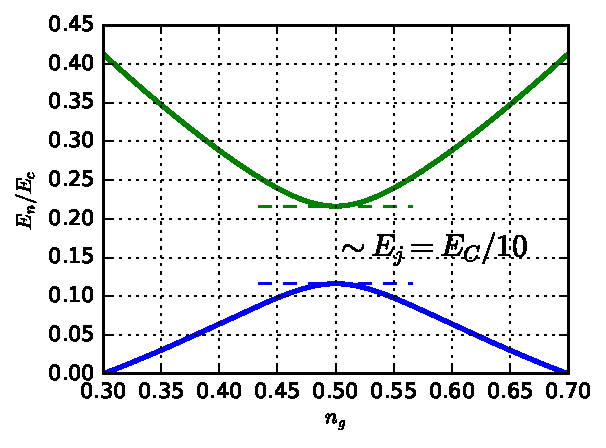
\includegraphics[height = .7\textwidth]{Pictures2/charge_qubit_05}
\caption{`` sweet spot '' -- область расщепления уровней, $n_g -1/2 \in \mathbb{Z}$}
\label{fig:charge-eigens-ng-2}
\end{subfigure}
\endgroup
\caption{Зависимость уровней энергии зарядового кубита от управляющего потенциала в виде $n_g$. Виден антикроссинг (?) и заметно отличие $\frac{\partial E_m}{\partial n_g}$ от нуля}
\label{fig:charge-eigens-ng}

\end{figure} 
\begin{figure}[!h]
\centering
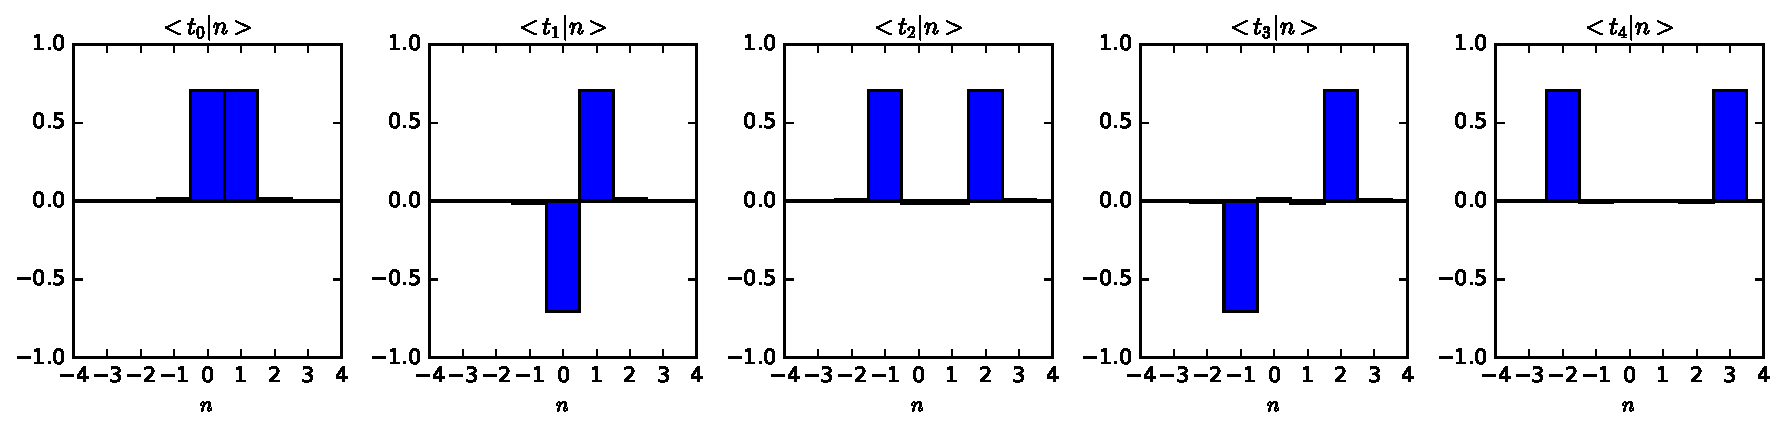
\includegraphics[width = 1\textwidth]{Pictures2/charge_2_eigenstates}
\caption{Собственные состояния зарядового кубита. В ``sweet spot'' они являются гибридизованными слабо возмущенными зарядовыми состояниями. }
\label{fig:charge-eigenstates}

\end{figure}

\pagebreak
\vfill
\subsection{Трансмон}
\paragraph{Зарядовый шум.} Для уменьшения зарядового шума необходимо увеличивать отношение $E_J / E_C$. Однако, это приводит к уменьшению \textit{ангармонизма} $\alpha \equiv E_{12} - E_{01}$. Ангармонизм не может быть нулевым, в этом случае у нас не будет изоляции первых двух уровней системы от остальных (в частности, совпадут энергии переходов $\ket{1} \rightarrow \ket{0}$ и $\ket{1} \rightarrow \ket{2}$). Так же, величина ангармонизма ограничивает скорость операций, производимых с помощью микроволновых импульсов [подробнее в ...].
\newline
Спасением является тот факт, что с уменьшием $E_C$ чувствительность к зарядовым шумам падает \textit{экспоненциально}, а ангармонизм всего лишь \textit{линейно} [ссылка]. Для достаточно больших $E_J/E_C$ зависимость $E_m(n_g)$ можно приблизить косинусом 
\begin{equation}
E_m\left(n_g\right) = E_m(n_g = 1/4) + \frac{\epsilon_m}{2}  \cos 2 \pi n_g 
\end{equation}
, где
\begin{equation}
\epsilon_m  = (-1)^m E_C \frac{2^{4m +5}}{m!} \sqrt{\frac{2}{\pi}} \left( \frac{E_J}{2 E_C} \right) ^ {\frac{m}{2} + \frac{3}{4}} \exp {\left( - \sqrt{8 E_J / E_C} \right)} 
\end{equation}
\linebreak
\begin{wrapfigure}{r}{0.5\textwidth}
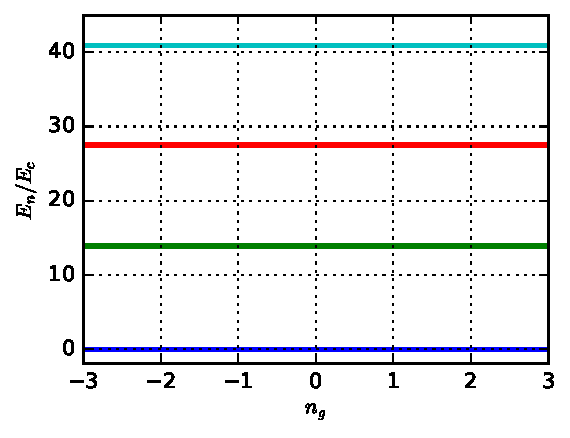
\includegraphics[width=0.5\textwidth ]{Pictures2/transmon_100}
\caption{При $E_J/E_C = 100$ $\epsilon_0 \sim 10^{-11}$ и зависимостью $E_m(n_g)$ можно пренебречь}
\label{fig:transmon-eigens}
\end{wrapfigure}
Для $E_J/E_C = 50$ получаем $\left|\epsilon_0\right| /  E_{01} \lesssim 10^{-8}$. При этом $E_{01} \simeq \sqrt{8 E_J E_C}$, а $\alpha \simeq - E_C$.
Для таких значений $\epsilon_m$ нет нужды в ``sweet spot'', а значит и механизма управления $n_g$. При моделировании трансмона можно положить $n_g = 0$. Оценим время дефазировки $T_2$, возникающей из-за зарядового шума в случае трансмона:
\begin{equation}
T_2 \sim \frac{\hbar}{A} \left|\frac{\partial E_{01}}{\partial n_g}\right|^{-1} \simeq \frac{\hbar}{e \pi \left| \epsilon_1 \right|}
\end{equation}
Используя возможные параметры трансмона $E_J = 30 ГГц, E_C = 0.35 ГГЦ$, получаем оценку времени жизни $T_2 = 400\mu s$. Для типичного зарядового кубита это время гораздо меньше -- $T_2 \sim 1\mu s$, что в частности и обуславливает широкую последующую популярность трансмона как физическую реализацию кубита. 
\newline
\paragraph{Анализ ???.} Рассмотрим собственные состояния трансмона (Рис. \ref{fig:transmon-eigenstates}). Для типичного $E_J / E_C = 100$ они еще не являются фазовыми состояниями ($\ket{\varphi} = \frac{1}{\sqrt{2 \pi}} \sum_n e^{i n \varphi} \ket{n}) $ и $\braket{t}{n}$ существенно затухает с ростом $n$ [wtf? как оценить падение $\braket{t}{n}$ ??]. Значит, можно использовать конечноразмерный гамильтониан трансмона в форме (\ref{eq:ham-qubit-charge-basis-N}).
\begin{figure}[!h]
\centering
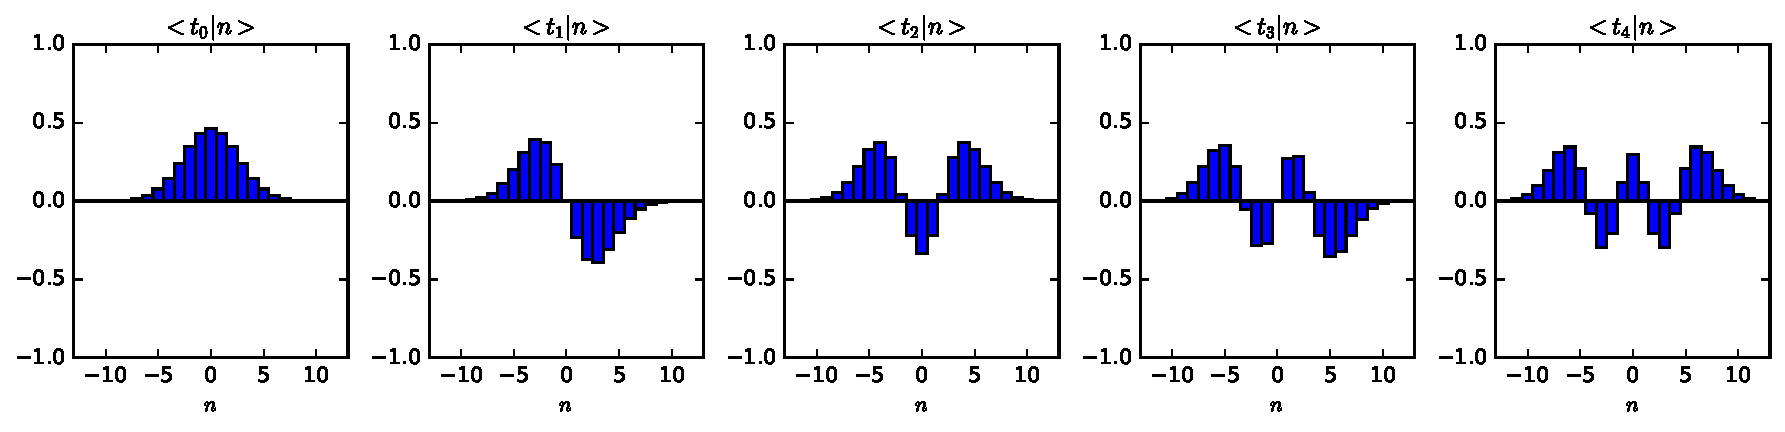
\includegraphics[width=1\textwidth]{Pictures2/transmon_eigenstates}
\caption{Собственные состояния трансмона $\ket{t}$ в зарядовом базисе $\ket{n}$}
\label{fig:transmon-eigenstates}
\end{figure}













\iffalse
\begin{figure}
\centering
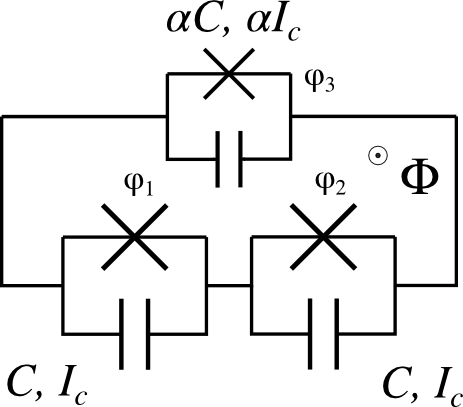
\includegraphics[width=0.4\textwidth]{Pictures/qubit}
\caption{Принципиальная схема Flux-кубита в рамках RCSJ-модели. Два из трех переходов по площади одинаковы, площадь третьего по сравнению с ними в $\alpha$ раз отличается (параметры отличаются в то же число раз согласно формулам для емкости конденсатора и (\ref{eq:Ic})). $\Phi$ -- поток, пронизывающий контур. Резисторы не изображены, так как рабочий ток переходов меньше $I_c$.}
\label{fig:qubit}
\end{figure}

 
Для трех невзаимодействующих переходов таких разностей будет три, и их и следует выбрать в качестве обобщенных координат системы. Однако в случае замкнутого контура дополнительно накладывается фазо-потоковое соотношение (\ref{eq:phsflx}):
\begin{equation}
\varphi_1 + \varphi_2 + \varphi_3 = 2\pi\left(\frac{\Phi}{\Phi_0} - k\right),\ k\in \mathcal{Z}.
\label{eq:qubit_phsflx}
\end{equation}
Таким образом, в контуре на \autoref{fig:qubit} остаются независимыми только две разности фаз из трех. Введя их в качестве обобщенных координат, можно понять, что является аналогом кинетической, а что -- потенциальной энергии системы. В уравнениях (\ref{eq:JJenrj1})-(\ref{eq:JJenrj2}) энергия перехода зависит непосредственно от $\varphi$, а емкостная от $\dot \varphi$. Таким образом, переход запасает потенциальную, а емкость кинетическую энергию. Энергия магнитного поля, возникающего при течении тока в кольце, считается малой в силу малости геометрической индуктивности кубита по сравнению с джозефсоновской индуктивностью переходов, а поток $\Phi \equiv \Phi_{ext}$ (подробное описание данной процедуры см. в статье \cite{Robertson2006}). Теперь можно записать лагранжиан системы, используя все те же уравнения (\ref{eq:JJenrj1})-(\ref{eq:JJenrj2}) и выражая разность фаз $\varphi_3$ отличающегося перехода через разности фаз $\varphi_1$ и $\varphi_2$ одинаковых переходов при помощи (\ref{eq:qubit_phsflx}):
\begin{gather*}
\mathcal{L} = \mathcal{T}-\mathcal{U}, \\
\mathcal{T} = E_{cap} =\frac{1}{2}\sum_{i=1}^3 C_i V_i^2 = \frac{1}{2} \left(\frac{\Phi_0}{2\pi}\right)^2 \left[C(\dot \varphi_1)^2 + \alpha C \left(\dot \varphi_1 + \dot\varphi_2\right)^2 + C(\dot \varphi_2)^2\right] \\
= \frac{1}{2}\left(\frac{\Phi_0}{2\pi}\right)^2 \left(\begin{matrix}
\dot\varphi_1 &\dot\varphi_2
\end{matrix}\right) C \left(\begin{matrix}
1+\alpha & \alpha \\
\alpha & 1+\alpha
\end{matrix}
\right)
\left(\begin{matrix}
\dot\varphi_1 \\
\dot\varphi_2
\end{matrix}\right),\\
\mathcal{U} = E_{ind} = E_J\left[2+\alpha - \cos\varphi_1 - \cos\varphi_2 - \alpha \cos\left(2\pi\frac{\Phi}{\Phi_0} - \varphi_1 - \varphi_2 \right)\right].
\end{gather*}
Строить гамильтониан системы из такого лагранжиана не очень удобно, поэтому предварительно произведем замену координат $\displaystyle \phi = \frac{\varphi_1 + \varphi_2}{2},\ \theta = \frac{\varphi_1 - \varphi_2}{2}$:
\begin{gather}
\mathcal{T}  \overset {\varphi_1, \varphi_2 \rightarrow \phi, \theta}{=}
C\left(\frac{\Phi_0}{2\pi}\right)^2 (\begin{matrix}
\dot \phi & \dot \theta
\end{matrix})
\left(\begin{matrix}
1+2\alpha & 0\\
0 & 1
\end{matrix}
\right)
\left(\begin{matrix}
\dot \phi \\ \dot \theta
\end{matrix}\right), \notag
\\
\mathcal{U} \overset {\varphi_1, \varphi_2 \rightarrow \phi, \theta}{=} E_J\left[2+\alpha - 2\cos(\phi)\cos(\theta) - \alpha\cos\left(2\pi\frac{\Phi}{\Phi_0} -2\phi\right)\right].
\label{eq:U_qb}
\end{gather}
Теперь, стандартным образом вводя обобщенный импульс 
$\displaystyle \mathbf{p}^T = \left(\begin{matrix}p_\phi & p_\theta\end{matrix}\right) = \left(\begin{matrix}\frac{\partial\mathcal{L}}{\partial\dot\phi} & \frac{\partial\mathcal{L}}{\partial\dot\theta}\end{matrix}\right)$ и производя преобразование Лежандра, получим итоговый гамильтониан системы:
\begin{gather*}
\mathcal{H} = \frac{p_\phi^2}{2M_\phi} + \frac{p_\theta^2}{2M_\theta}+ E_J\left[2+\alpha - 2\cos(\phi)\cos(\theta) - \alpha\cos\left(2\pi\frac{\Phi}{\Phi_0} -2\phi\right)\right], \\
M_\phi = 2C\left(\frac{\Phi_0}{2\pi}\right)^2(1+2\alpha),\ M_\theta = 2C\left(\frac{\Phi_0}{2\pi}\right)^2.
\end{gather*}
Далее, осуществляя переход к операторному виду квантовой механики, можно получить оператор Гамильтона для сверхпроводящего потокового кубита в терминах исключительно $E_C$ и $E_J$:
\begin{equation}
\begin{gathered}
\hat{\mathcal{H}} = E_C\left[-\frac{1}{2(1 + 2\alpha)}\frac{\partial^2}{\partial\phi^2} 
- \frac{1}{2}\frac{\partial^2}{\partial\theta^2}\right] + \\ + E_J\left[2+\alpha - 2\cos(\phi)\cos(\theta) - \alpha\cos\left(2\pi\frac{\Phi}{\Phi_0} -2\phi \right)\right].
\end{gathered}
\label{eq:hamiltonian}
\end{equation}

\subsection{Квантово-механический анализ}

\begin{figure}[!p]

\begingroup
\captionsetup[subfigure]{width=0.9\textwidth, justification=normal}
\centering
\begin{subfigure}[t]{0.49\linewidth}
\centering
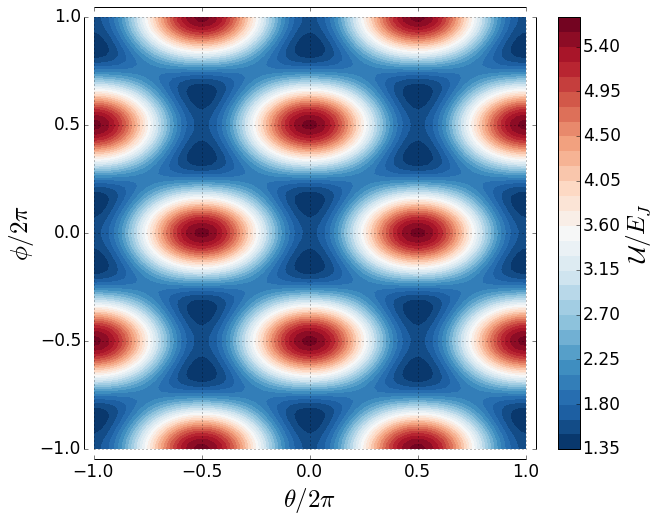
\includegraphics[height = .8\textwidth]{Pictures/qubit_potential}
\caption{Трехмерное изображение потенциала при $\Phi = \Phi_0/2,\ \alpha=0.8$. Можно видеть $2\pi$-периодическую центрированную квадратную решетку с базисом из двойных ям.}
\label{fig:U3d}
\end{subfigure}~
\begin{subfigure}[t]{0.49\linewidth}
\centering
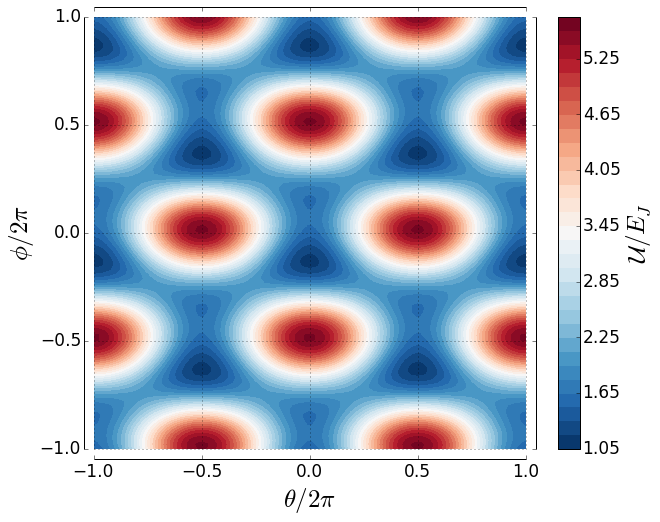
\includegraphics[height = .8\textwidth]{Pictures/qubit_potential2}
\caption{При отклонении потока от $\Phi_0/2$ появляется перекос внутри двойных ям, одна половина становится глубже, а другая мельче в зависимости от знака отклонения $\Delta\Phi$. Здесь $\Delta\Phi=-0.05\Phi_0,\ \alpha=0.8$}
\label{fig:U3d2}
\end{subfigure}

\vspace{1cm}
\begin{subfigure}[t]{0.49\linewidth}
\centering
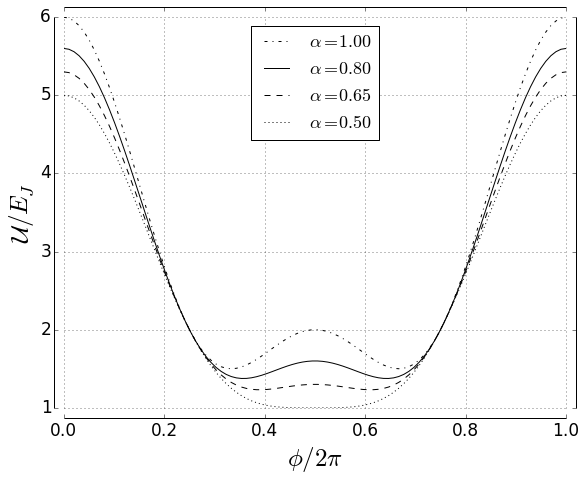
\includegraphics[height = 0.8\textwidth]{Pictures/qubit_potential_cut}
\caption{Срез потенциала при $\Phi = \Phi_0/2$ по направлению $\theta = \pi$ (барьер внутри ям) в зависимости от $\alpha$. При $\alpha = 0.5$ этот барьер пропадает, при $\alpha=1$ он сравнивается с барьером между ямами (см. (\subref{fig:U_cut2})).}
\label{fig:U_cut}\quad
\end{subfigure}
\begin{subfigure}[t]{0.49\linewidth}
\centering
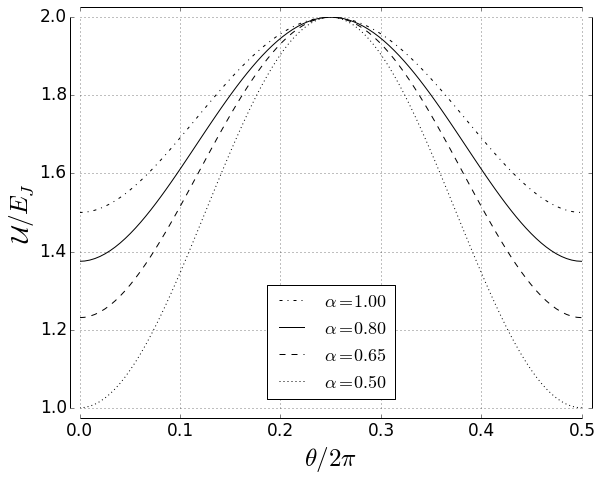
\includegraphics[height = 0.8\textwidth]{Pictures/qubit_potential_cut2}
\caption{Срез потенциала при $\Phi = \Phi_0/2$ по направлению $\phi = \left(1 - \frac{2}{\pi}\arccos
\frac{1}{2\alpha}\right)\theta+\arccos\frac{1}{2\alpha}$ (барьер между ямами) в зависимости от $\alpha$. Здесь крайние точки отвечают минимумам $\mathcal{U}$ при $\theta=0\ (\pi),\ \phi=\arccos
\frac{1}{2\alpha}\ \left(\pi - \arccos\frac{1}{2\alpha}\right)$.}
\label{fig:U_cut2}
\end{subfigure}
\endgroup
\caption{Графическое изображение периодического потенциала Flux-кубита в зависимости от относительного размера отличающегося перехода $\alpha$ и пронизывающего потока $\Phi$.}
\label{fig:U_fq}
\end{figure} 

\paragraph{Анализ потенциала.} Прежде всего рассмотрим потенциал $\mathcal{U}(\phi, \theta)$. На \autoref{fig:U_fq} представлены графики, демонстрирующие его структуру в случае $\Phi = \Phi_0/2$, или в так называемой \textit{точке вырождения} по потоку. На \autoref{fig:U_fq}~(\subref{fig:U3d}) можно видеть, что потенциал $2\pi$-периодичен по каждой из переменных $\phi$ и $\theta$ и представляет собой бесконечную центрированную квадратную решетку с базисом из симметричных двойных ям, отделенных друг от друга диагональными барьерами. Каждая их ям, в свою очередь, делится на две части меньшим барьером. Его высота, как видно из \autoref{fig:U_fq}~(\subref{fig:U_cut}), определяется параметром $\alpha$. Для того, чтобы структура оставалась подобной изображенной на \autoref{fig:U_fq}~(\subref{fig:U3d}), требуется, чтобы $\alpha\in(0.5,\ 1)$: при нарушении этого условия либо совсем пропадает внутренний барьер, либо внешний барьер сравнивается с внутренним по высоте, и ямы перестают быть качественно отделены друг от друга (\autoref{fig:U_fq}~(\subref{fig:U_cut2})). Минимумы $\mathcal{U}$ находятся в точках $\theta=\pi k,\ \phi=\pm\arccos\frac{1}{2\alpha}+\pi \frac{n}{2},\ k,\ n\in\mathcal{Z}$, причем в точке вырождения все минимумы имеют одинаковую энергию, а при отходе от нее в зависимости от знака отклонения одна половина двойных ям становится мельче, а другая глубже, и вырождение внутри каждой ямы снимается (\autoref{fig:U_fq}~(\subref{fig:U3d2})). 

\begin{figure}[!p]
\begingroup
\captionsetup[subfigure]{width=\textwidth}
\centering
\begin{subfigure}[t]{0.75\linewidth}
\centering
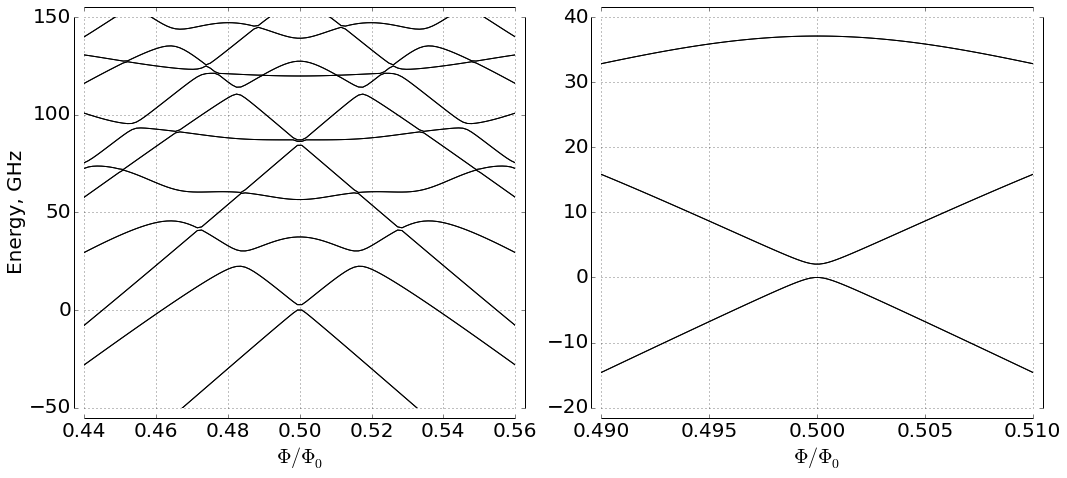
\includegraphics[width = \textwidth]{Pictures/qubit_levels}
\caption{Уровни энергии в зависимости от внешнего поля. Каждая линия на рисунке на самом деле является двойной (подробности см. в тексте).}
\label{fig:levels}
\end{subfigure}

\begin{subfigure}[t]{0.8\linewidth}
\centering
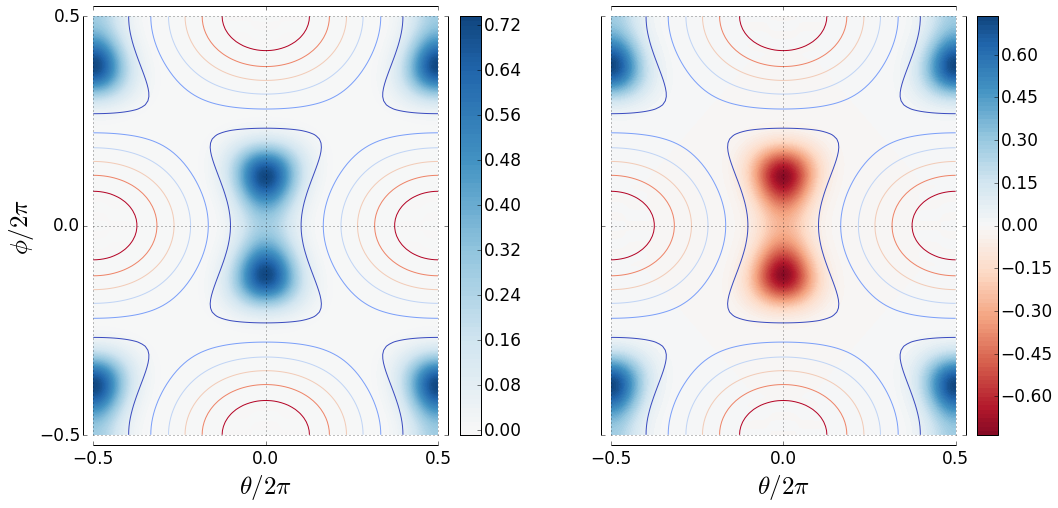
\includegraphics[width = \textwidth]{Pictures/wfs01}
\caption{Граничные по квазиимпульсу состояния нулевой зоны (``$\ket{g}$-состояния'') в точке вырождения. Внутри ям волновая функция четная.}
\label{fig:wfs01}
\end{subfigure}

\begin{subfigure}[t]{0.8\linewidth}
\centering
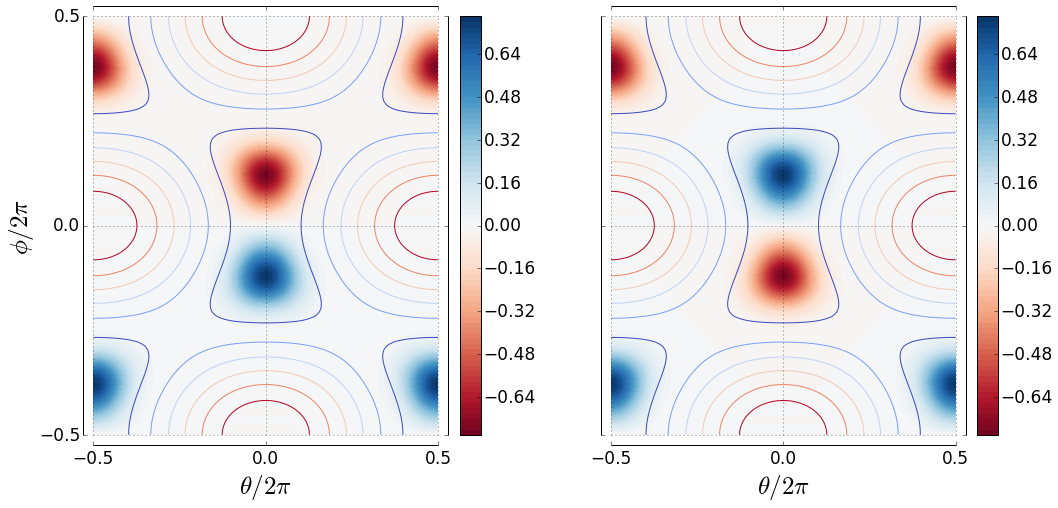
\includegraphics[width = \textwidth]{Pictures/wfs23}
\caption{Граничные по квазиимпульсу состояния первой зоны (``$\ket{e}$-состояния'') в точке вырождения. Внутри ям волновая функция нечетная.}
\label{fig:wfs23}
\end{subfigure}

\endgroup
\caption{Результаты численного решения стационарного уравнения Шредингера с параметрами $\alpha=0.7,\ E_J  = 30E_C = 400\ \text{GHz}$. Цветом обозначено значение волновой функции, нормированной на единицу в периоде потенциала.}
\label{fig:numerical_res}
\end{figure} 

\paragraph{Стационарные состояния.} Прежде, чем начинать поиск стационарных состояний для гамильтониана (\ref{eq:hamiltonian}), важно не упустить смысл происходящего. Строго говоря, в силу того, что потенциал (\ref{eq:U_qb}) является периодическим, решениями уравнения Шредингера будут являться \textit{блоховские функции}, а спектр энергий будет иметь зонную структуру. Таким образом, в приближении нулевой индуктивности Flux-кубит представляет собой модель частицы в идеальной периодической решетке двумерного твердого тела. В реальности, однако, энергетический спектр все же является дискретным из-за квадратичной по фазам индуктивной энергии\cite{Robertson2006}, с пиками числа уровней в областях бывших зон. 

Оставаясь в рамках приближения нулевой индуктивности, для аналитического решения задачи можно использовать модель сильной связи для центрированной решетки с базисом, однако мы будем рассматривать численный вариант -- метод, изложенный в работе\cite{Johansson}. В условиях $2\pi$-периодичности и действительности потенциала и искомой волновой функции можно разложить в ряд Фурье, ограничиваясь $2N+1$ начальными слагаемыми, уравнение Шредингера с гамильтонианом (\ref{eq:hamiltonian}), что после определенных преобразований сведет задачу к поиску собственных значений и векторов матрицы размером $(2N+1)^2$ на $(2N+1)^2$. Результаты такого вычисления для $N=20$ представлены на \autoref{fig:numerical_res}. Вычисленный спектр энергий (\autoref{fig:numerical_res}~(\subref{fig:levels})) состоит из дублетов (на рисунке они сливаются в синглеты), причем расщепление в дублетах обусловлено разными периодическими конфигурациями волновой функции при фиксированной четности ее внутри ям, а расстояния между дублетами изменением четности внутри ям. Такая структура спектра возникает по причине того, что в силу использованных предположений о волновой функции машинный метод ``вылавливает'' из каждой энергетической зоны лишь граничные состояния, так как только они обладают вышеуказанными свойствами. Действительно, по теореме Блоха $\psi(r) = e^{ikR}\psi(r)$, для граничных квазиимпульсов $k = 0$  и $k = K/2$ ($K$ -- вектор обратной решетки) выполнено соответственно $\psi(r+R) = \psi(r)$ и $\psi(r+R)=-\psi(r)$, что и наблюдается на парах \autoref{fig:numerical_res}~(\subref{fig:wfs01}) и \autoref{fig:numerical_res}~(\subref{fig:wfs23}). Четные конфигурации волновой функции имеют меньшую рассчитанную энергию, а нечетные большую, в соответствии с вышесказанным.

В зависимости от поля спектр ведет себя, как показано на \autoref{fig:numerical_res}~(\subref{fig:levels}), неравномерно: в окрестности $\Phi_0/2$ четные зоны сдвигаются вниз, нечетные вверх, а на большем удалении магнитного потока от полкванта картина вообще теряет порядок из-за значительного числа квазипересечений. На \autoref{fig:numerical_res}~(\subref{fig:wfs01}) и (\subref{fig:wfs23}) изображены соответственно нулевое и первое дублетные состояния в точке вырождения.  Далее мы будем пренебрегать тем, что первые две зоны отличны от дискретных уровней, так как расщепления внутри них примерно в $10^5$ раз меньше, чем расстояния между ними, и назовем верхнюю по энергии зону ``$\ket{e}$-состоянием'', а нижнюю ``$\ket{g}$-состоянием''.

\paragraph{Двухуровневое приближение.} Следующим шагом будет приведение системы к двум нижним состояниям, пренебрегая всеми остальными. Это оправданно, так как третья зона в окрестности точки вырождения лежит гораздо выше (почти в 20 раз) по энергии, чем состояние $\ket{e}$ . Теперь, используя метод сильной связи в двойной яме, рассчитаем зависимость расщепления уровней $\ket{g}$ и $\ket{e}$ от $\Phi$. Разобьем яму на два потенциала $\mathcal{U}_1$ и $\mathcal{U}_2$, так, что их сумма даст исходный потенциал ямы, а не равными нулю они окажутся только в области соответствующих полуям. Для каждого из этих двух потенциалов можно найти основные состояния, которые мы обозначим $\ket{1, g}$ и $\ket{2, g}$. Основное состояния для уравнения с потенциалом $\mathcal{U}_1+\mathcal{U}_2$ в предположении о малом перекрытии потенциалов и волновых функций отдельных ям можно искать в виде $\ket{g} = a\ket{1, g} + b\ket{2, g}$. Также мы получим сразу и $\ket{e}$ в качестве второго решения задачи. Итак, записывая полный гамильтониан, действуя им на выбранного вида функцию $\ket{g}$ и умножая слева сначала на $\bra{1, g}$, а потом на $\bra{2, g}$, получим следующую систему уравнений:
\begin{align*}
\left(\begin{matrix}
E_{1g}+U_2^{1g1g} & E_{1g}\braket{1,g}{2,g} + U_2^{1g2g}\\ 
E_{2g}\braket{2,g}{1,g} + U_1^{2g1g} & E_{2g} + U_1^{2g2g}
\end{matrix}\right) 
\left(\begin{matrix}
a \\b 
\end{matrix}\right) = 
E\left(\begin{matrix}
1 & \braket{1,g}{2,g} \\
\braket{2,g}{1,g} & 1
\end{matrix}\right)
\left(\begin{matrix}
a \\b 
\end{matrix}\right),
\end{align*}
где верхними индексами обозначены соответствующие матричные элементы потенциалов $U$, $E_{1g}, E_{2g}$ -- энергии основных состояний ям, $E$ -- искомое собственное значение полного гамильтониана. Далее, пренебрежем диагональными матричными элементами потенциалов, так как здесь они берутся по волновым функциям противоположной половины ямы, а также неортогональностью $\ket{1, g}$ и $\ket{2, g}$ (они также локализованы в разных ямах). Тогда уравнение значительно упростится:
\begin{align*}
\left(\begin{matrix}
E_{1g} &  U_2^{1g2g}\\ 
U_1^{2g1g} & E_{2g}
\end{matrix}\right) 
\left(\begin{matrix}
a \\b 
\end{matrix}\right) = 
E
\left(\begin{matrix}
a \\b 
\end{matrix}\right).
\end{align*}
Следующим приближением будет пренебрежение различием в недиагональных элементах, так как при малых отклонениях $\Phi$ деформации около дна ям незначительны, и можно считать, что формы волновых функций и потенциалов остаются прежними, а меняются лишь энергии основных состояний из-за перекоса ям. Переобозначая элементы матрицы и смещая собственные значения на постоянную величину, получаем сокращенный гамильтониан следующего вида:
\begin{equation}
\begin{gathered}
\mathcal{\hat H} = \frac{\hbar \varepsilon}{2} \hat\sigma_z + \frac{\hbar \Delta}{2} \hat \sigma_x \Leftrightarrow \frac{\hbar \varepsilon}{2} \hat\sigma_x + \frac{\hbar\Delta}{2} \hat \sigma_z \\ 
\text{(с точностью до выбора базиса)} 
\end{gathered}
\label{eq:trunc_hamiltonian} 
\end{equation}
где $\hbar \Delta = 2 U_1^{2g1g} \approx 2U_2^{1g2g}$ -- минимальное расщепление по энергии, $\hbar \varepsilon = |E_{1g} - E_{2g}|$ -- сдвиг энергий основных состояний ям в зависимости от поля. После дифференцирования потенциала можно получить, что сдвиг минимумов по энергии, а, следовательно, и $\varepsilon$, будут пропорциональны $\Phi - \Phi_0/2$.

Сокращенный гамильтониан \eqref{eq:trunc_hamiltonian} можно просто привести к диагональному виду. Его собственные значения и их разность будут зависеть от $\varepsilon$ следующим образом:
\begin{equation}
E_{g, e} = \pm \frac{\hbar}{2}\sqrt{\Delta^2 + \varepsilon^2},\
\Delta E = h \nu_q = \hbar \omega_q = \hbar\sqrt{\Delta^2 + \varepsilon^2},
\end{equation}
где $\nu_q$ -- это экспериментально наблюдаемая частота перехода между кубитными уровнями. Легко построить зависимость этой частоты от приложенного поля -- это гипербола.

Главным обоснованием сделанных приближений является точный численный результат \autoref{fig:numerical_res}~(\subref{fig:levels}) для двух нижних состояний, который так же дает гиперболическую зависимость.

\section{Открытые системы и декогеренция}

Переход от замкнутых квантовых систем, эволюция которых подчинена нестационарному уравнению Шредингера и состояние которых в каждый момент времени точно известно, к так называемым \textit{открытым}, т.е. незамкнутым, квантовым системам всегда сопряжен с трудностями. Это связано с тем, что для описания таких систем в идеале требовалось бы найти закон эволюции Вселенной, а затем исключить из рассмотрения все ее степени свободы, не касающиеся представляющей интерес области. Эта формулировка является, конечно, довольно туманной в отношении Вселенной, но что вообще такое Вселенная? В силу отсутствия однозначного ответа на данный вопрос в качестве ``вселенной'' часто выбирают что-то простое, такое, что в определенных приближениях можно описать математически -- и получают результаты, очень хорошо согласующиеся с экспериментом\cite{bishop2009}. Далее будет описана такая процедура и соответствующий математический аппарат.

\subsection{Матрица плотности}

Матрица плотности -- это обобщение вектора состояния на системы, точное состояние которых неизвестно. Матрицы плотности подразделяются на \textit{чистые} и \textit{смешанные}: первые эквивалентны обычной волновой функции, вторые же определяют распределение вероятности на волновых функциях. Рассмотрим две ситуации:
\begin{enumerate}
\item Система находится в суперпозиции состояний из какого-либо набора $\ket{a} = \sum_k c_k \ket{k}$. Тогда матрица плотности является чистой и записывается следующим образом: 
\[ \hat \rho_a = \ket{a}\bra{a} = \sum_{k,n}c_k c_n^* \ket{k}\bra{n}.\]
\item Система находится в каком-то одном из состояний $\ket{k}$ с вероятностью $|c_k|^2$. Тогда матрица плотности является смешанной и записывается теперь иначе:
\[ 
\hat \rho_a = \sum_k |c_k|^2 \ket{k}\bra{k}.
\]
\end{enumerate}
В чем удобство таких определений? Для ответа на этот вопрос рассмотрим значение произвольной наблюдаемой с оператором $\hat Q$. В первом случае, из определения:
\[
Q = \bra{a}\hat Q\ket{a} = \sum_{k,n} c_k c_n^* \bra{n}\hat Q\ket{k}\ \equiv \sum_i \sum_{k,n} c_k c_n^* \braket{i}{k} \bra{n} \hat Q \ket{i} \overset{def}{=}\Tr{\hat \rho_a \hat Q}. 
\]
Во втором случае, из определения и квантового, и статистического среднего, а также приема, примененного выше, для каждого вероятного состояния:
\[
Q = \sum_k Q_k |c_k|^2 = \sum_k \Tr{ \ket{k}\bra{k} \hat Q} |c_k|^2 \equiv \Tr{\hat \rho_a \hat Q}. 
\]
Таким образом, через матрицу плотности мы получаем единое определение среднего значения оператора, имеющего смысл как для статистического, так и для простого квантового случая. Также просто показывается, что обе матрицы плотности удовлетворяют одному и тому же \textit{уравнению Лиувилля-фон-Неймана}: 
\[ 
i\hbar \frac{\partial}{\partial t} \hat \rho = [\mathcal{\hat H}, \hat \rho].
\]

В качестве примера того, как матрица плотности может помочь при описании открытых систем, рассмотрим два кубита, находящихся в \textit{перепутанном} состоянии, когда невозможно представить их общее состояние как тензорное произведение векторов состояний кубитов по отдельности. Такое состояние -- это, например, 
\[
\ket{\Psi^+} = \frac{1}{\sqrt{2}}(\ket{\uparrow}_A\otimes\ket{\downarrow}_B+\ket{\downarrow}_A\otimes\ket{\uparrow}_B).
\]
Соответствующая матрица плотности:
\[ 
\hat \rho_{\Psi^+} = \frac{1}{2} \rbrkt{\begin{matrix}
0&0&0&0\\
0&1&1&0\\
0&1&1&0\\
0&0&0&0
\end{matrix} }.
\]
Каждый из кубитов в примере является, по сути, открытой системой, которую требуется описать. Для этого вводится понятие \textit{сокращенной матрицы плотности} и операция взятия \textit{частичного следа} для системы из двух подсистем:
\[
\hat \rho_A = \pTr{B}{\hat \rho_{AB}} \overset{def}{=} \sum_i \bra{i}_B \hat \rho_{AB} \ket{i}_B \ \Leftrightarrow \ [\hat \rho_A]_{n, m} = \sum_i \bra{n}_A \! \otimes\! \bra{i}_B\ \hat \rho_{AB}\ \ket{i}_B\!\otimes\! \ket{m}_A,
\] 
где суммирование ведется по базису подсистемы B (второе выражение показывает, как суммировать по состояниям композитного базиса $A\otimes B$). Для каждого из двух кубитов системы в состоянии $\ket{\Psi^+}$ такое вычисление даст $\hat \rho_{A,B} = \mathbbm{\hat 1}_{A, B}/2$: сокращенная матрица плотности каждого из них смешанная и дает 50\%-ую вероятность быть в одном из двух состояний. Таким образом, зная все о перепутанной системе, мы не имеем достоверной информации о ее частях.

\subsection{Уравнение эволюции в форме Линдблада}

Процедура сокращения матрицы плотности, проведенная с двумя кубитами и их общим стационарным состоянием, применяется и в нестационарном случае для получения \textit{основного уравнения эволюции подсистемы} (master equation for the subsystem)\cite{carmichael1999}. Исходный гамильтониан включает систему, ее окружение и их взаимодействие:
\begin{gather}
\mathcal{\hat H}_{se} = \mathcal{\hat H}_s \otimes \mathbbm{\hat 1}_e + \mathbbm{\hat 1}_s \otimes \mathcal{\hat H}_e + \mathcal{\hat H}_i. 
\label{eq:H_se}
\\
i\hbar \frac{\partial}{\partial t} \hat \rho_{se} = [\mathcal{\hat H}_{se}, \hat \rho_{se}]
\label{eq:se_se}
\end{gather}
Теперь обозначим приближения, которые используются для получения сокращенного уравнения эволюции (хорошее обсуждение их соответствия реальности см. в работе \cite{rivas2010}):
\begin{enumerate}
\item \textbf{Модель окружения.} В качестве модели внешней среды обычно используется бозе-термостат, т.е. $  \mathcal{\hat H}_e = \sum_k \hbar \omega_k \hat a_k^\dag \hat a_k$ в \eqref{eq:H_se}, а взаимодействие $\mathcal{\hat H}_i$ однобозонным и слабым.
\item \textbf{Борновское приближение.} При решении уравнения \eqref{eq:se_se} мы ищем матрицу плотности системы в виде $\hat \rho_{se}(t) = \hat \rho_{s}(t) \otimes \hat \rho_{e}^0$, тем самым пренебрегая изменением состояния термостата $\displaystyle \hat \rho_{e}^0 = \exp\rbrkt{-\beta \mathcal{\hat H}_{e}}/\Tr{\exp\rbrkt{-\beta \mathcal{\hat H}_e}},\ \beta = 1/kT$.
\item \textbf{Приближение Маркова.} Эволюция $\hat \rho_{s}$ после момента $t$ определяется только ее значением в этот момент и не зависит от прошлых значений. По-другому это формулируется как отсутствие памяти у термостата. 
\end{enumerate}
В условиях выбранных приближений можно путем достаточно громоздких преобразований получить уравнение динамики подсистемы. Его часть, ведущая к отличиям от стандартной унитарной эволюции, окажется представимой в \textit{форме Линдблада}, и, в итоге, искомое уравнение будет иметь следующий вид:

\begin{gather}
 \frac{\partial}{\partial t}\hat \rho_s = \frac{i}{\hbar} \sbrkt{\hat \rho_s, \mathcal{\hat H}_s} +
\sum_k \Gamma_k \rbrkt{\mathcal{\hat O}_k \hat \rho_s \mathcal{\hat O}_k^\dag - \frac{1}{2} \left\{ \mathcal{\hat O}_k^\dag \mathcal{\hat O}_k, \hat \rho_s \right\} } \notag \\
\overset{def}{=} \frac{i}{\hbar}\sbrkt{\hat \rho_s, \mathcal{\hat H}_s} + \sum_k \Gamma_k \mathcal{D}\sbrkt{\mathcal{\hat O}_k}\hat \rho_s.
\label{eq:gen_lind}
\end{gather}
$\mathcal{\hat D}$ - линдбладовский супероператор. Коэффициенты $\Gamma_k$, определяющие скорость распада, и операторы $\mathcal{\hat O}_k$, определяющие каналы распада, выводятся\cite{carmichael1999} для каждой конкретной модели, для каждого гамильтониана \eqref{eq:H_se}, однако вид \eqref{eq:gen_lind} сохраняется (это можно показать в рамках теории квантовых полугрупп, что и сделал Линдблад\cite{lindblad1976}). Далее будут рассматриваться явные выражения диссипативных членов для кубита. Выражения для квантового осциллятора выводятся похожим образом, их можно найти в литературе.\cite{carmichael1999}

\subsection{Релаксация}

Для получения диссипатора, отвечающего за передачу энергии кубита внешнему бозе-полю, используется следующий модельный гамильтониан:

\begin{equation}
\mathcal{\hat H}_{se} = \frac{\hbar \omega_q}{2} \hat \sigma_z \otimes \mathbbm{\hat 1}_e + \mathbbm{\hat 1}_q \otimes  \sum_k \hbar \omega_k \hat a_k^\dag \hat a_k  + \sum_k \hbar g_k \rbrkt{\hat \sigma^-\otimes \hat a_k^\dag +  \hat \sigma^+ \otimes \hat a_k},
\label{eq:rel_model}
\end{equation}
где $\omega_q, \omega_k$ -- энергии кубита и мод, $\hat \sigma^{\pm}$ -- повышающий и понижающий операторы кубита, $\hat \sigma^+ = \hat{\sigma}^{-^\dag} = \ket{e}\bra{g}$, а $g_k$ -- константы связи кубита с внешним полем. Последняя часть возникает из взаимодействия квантованного поля каждой моды, которое пропорционально $\hat a_k^+ + \hat a_k$, с кубитом (через оператор $\hat \sigma_x = \hat \sigma^-+  \hat \sigma^+ $, см. \eqref{eq:trunc_hamiltonian}) в первом порядке теории возмущений, т.е. $\mathcal{\hat H}_{i_k} \propto \rbrkt{\sigma^-+  \hat \sigma^+}\otimes\rbrkt{\hat a_k^+ + \hat a_k}\overset{\mathbb{I}\, ord.}{\rightarrow} (\hat \sigma^-\otimes \hat a_k^\dag +  \hat \sigma^+ \otimes \hat a_k)$. Это оправданно, так как мы полагаем связи, т.е. $g_k$, малыми, а основные поправки к поведению системы исходящими от мод с $\omega_k\approx \omega_q$ (подробнее см. \autoref{subsec:rabi_specrum}). Исходя из такой модели при $T \approx 0$ получаем\cite{carmichael1999} следующее уравнение эволюции:
\begin{equation}
\frac{\partial}{\partial t}\hat \rho_q = \frac{i}{\hbar} \sbrkt{\hat \rho_q, \mathcal{\hat H}_q} +
\gamma (\hat \sigma^- \hat \rho_q \hat \sigma^+ - \frac{1}{2} \left\{ \hat\sigma^+\hat\sigma^-, \hat \rho_q \right\} ),
\end{equation}
где $\gamma$ получается в процессе вычисления из \eqref{eq:rel_model}, однако на практике подгоняется к экспериментальным данным. Строго говоря, частота кубита при выводе окажется измененной (\textit{лэмбовский сдвиг}), однако этим  изменением можно пренебречь. Динамика данного уравнения будет обсуждаться ниже.

\subsection{Чистая дефазировка}

Более тонкий эффект может быть получен, если рассматривать другую модель, выбрав следующий вид гамильтониана \eqref{eq:H_se}\cite{carmichael1999}:

\begin{align}
\mathcal{\hat H}_{q} &= \frac{\hbar \omega_q}{2} \hat \sigma_z \otimes \mathbbm{\hat 1}_e \notag \\
\mathcal{\hat H}_{e} &= \mathbbm{\hat 1}_s \otimes \sum_k \hbar \omega_{1k} \hat a_{1k}^\dag \hat a_{1k}  + \mathbbm{\hat 1}_s \otimes \sum_k \hbar \omega_{2k} \hat a_{2k}^\dag \hat a_{2k} 
\label{eq:deph_model}
\\
\mathcal{\hat H}_i &= \sum_{k,j} \hbar g_{k,j} \rbrkt{\hat \sigma^-\hat\sigma^+ \otimes \hat a_{1k}^\dag \hat a_{1j} +  \hat \sigma^+\hat\sigma^- \otimes \hat a_{2k}^\dag \hat a_{2j}} \notag.
\end{align}	
Слагаемое $\mathcal{\hat H}_i$ здесь отвечает за переброс мод термостата вместе с виртуальным возбуждением (релаксацией) кубита. Так же выбирается иногда т. н. спин-бозонное взаимодействие\cite{leggett1987}. Различные варианты получаются в общем случае из разложения произвольного оператора в пространстве термостата по фундаментальным модам\cite{hsu1987}. Аналогично предыдущему пункту, получаем следующее уравнение:
\begin{equation}
\frac{\partial}{\partial t}\hat \rho_q = \frac{i}{\hbar}\sbrkt{\hat \rho_q, \mathcal{\hat H}_q} +
\frac{\gamma_\phi}{2} (\hat \sigma^z \hat \rho_q \hat \sigma^z - \frac{1}{2} \left\{ \hat\sigma^z\hat\sigma^z, \hat \rho_q \right\} ) \equiv \frac{i}{\hbar}\sbrkt{\hat \rho_q, \mathcal{\hat H}_q} +
\frac{\gamma_\phi}{2} (\hat \sigma^z \hat \rho_q \hat \sigma^z -\hat \rho_q ),
\end{equation}
где последнее равенство верно в силу того, что $\hat \sigma_z^2 \equiv \mathbbm{\hat 1}$. Понятно, что объединив гамильтонианы \eqref{eq:rel_model} и \eqref{eq:deph_model}, мы получим итоговое уравнение с диссипативной частью $\gamma\mathcal{D} \sbrkt{\hat \sigma^- }+\frac{\gamma_\phi}{2} \mathcal{D} \sbrkt{\hat \sigma_z} $. Теперь перейдем к рассмотрению динамики таких уравнений.



\subsection{Диссипативная динамика}

Качественный вид картины диссипации сильно зависит от выбранного начального состояния системы: на основное состояние диссипаторы не оказывают влияния вовсе, а, например, на возбужденное оказывает влияние только релаксация, экспоненциально ``спуская'' его по вертикальной оси сферы Блоха. 

\begin{figure}[h]
\centering
\begin{subfigure}[t]{0.32\textwidth}
\centering
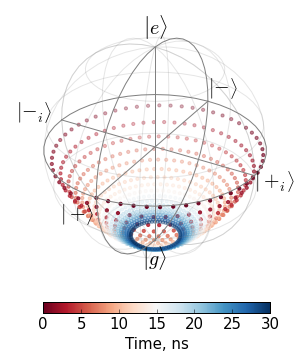
\includegraphics[width=0.95\textwidth]{Pictures/bloch_rel}
\caption{Релаксация,\\ $\gamma = 0.1,\ \gamma_\phi = 0$}
\end{subfigure}
\begin{subfigure}[t]{0.32\textwidth}
\centering
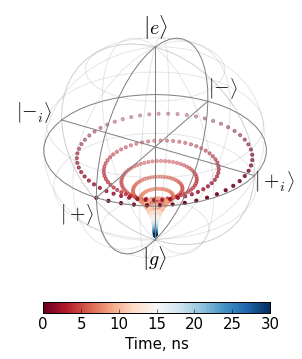
\includegraphics[width=0.95\textwidth]{Pictures/bloch_tot}
\caption{Общий эффект, \\$\gamma = \gamma_\phi = 0.1$}
\end{subfigure}
\begin{subfigure}[t]{0.32\textwidth}
\centering
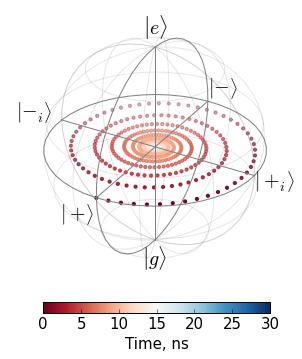
\includegraphics[width=0.95\textwidth]{Pictures/bloch_deph}
\caption{Дефазировка, \\ $\gamma = 0,\ \gamma_\phi = 0.1$}
\end{subfigure}
\caption{Диссипативная динамика кубита с $\nu_q$=1 ГГц.}
\label{fig:bloch}
\end{figure}

Для состояния $\ket{+} = \frac{1}{\sqrt{2}}(\ket{e}+\ket{g})$ более интересная картина эволюции представлена на \autoref{fig:bloch}. Как видно, дефазировка уничтожает когерентность суперпозиции, т.е. приближает значение $\Tr{\hat \rho_q^2}$ к 1/2, в то время как релаксация проходит от чистого до смешанного состояния, а затем возвращается к чистому $\ket{g}$.


\subsection{Вынужденное поведение} \label{subsec:driven_qubit}

Практический интерес представляет \textit{когерентное} взаимодействие кубита с контролирующими импульсами, которые по сути так же являются внешними, однако сохраняют чистоту состояния. В рамках теории Flux-кубита возмущением является синусоидально изменяющийся магнитный поток, проходящий через кольцо. В случае рассмотрения вынужденного поведения можно использовать классический подход в отношении поля и записывать оператор возмущения для кубита как $\mathcal{\hat V}_q = \hbar f_q \hat \sigma_x \cos\omega t$, где $f_q$ -- это (с точностью до множителя) амплитуда изменения магнитного потока, а $\omega$ -- частота. Если моделировать эволюцию кубита под таким возмущением, то получится изображенная на \autoref{fig:rabi_osc} динамика. Видно, что чем слабее возмущение, тем ближе к гармоническим оказываются колебания $\left<\hat \sigma_z\right>$ -- \textit{осцилляции Раби}. Частота этих осцилляций пропорциональна амплитуде переменного поля, однако при значительном увеличении амплитуды они перестают быть периодическими. Аналитически рассматриваться поведение системы может в 
\textit{приближении вращающейся волны}\cite{Jerger2013, Bishop2010, Bauer2006} (Rotating Wave Approximation, RWA), которое убирает вращение вокруг оси $Oz$: $ (\hat \sigma^+ + \hat \sigma^-)(e^{i\omega t}+e^{-i\omega t}) \rightarrow (\hat \sigma^- e^{-i\omega t} + \hat \sigma^+ e^{i\omega t})$, а также, при длительном воздействии возмущения, по теории Флоке\cite{Bauer2006}. 
\begin{figure}[h!]
\centering
\begin{subfigure}[t]{0.4\textwidth}
\centering
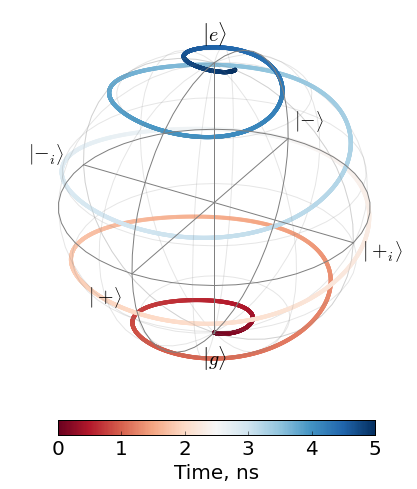
\includegraphics[height=0.22\textheight]{Pictures/rabi_dynamics_bloch}
\end{subfigure}\quad
\begin{subfigure}[t]{0.5\textwidth}
\centering
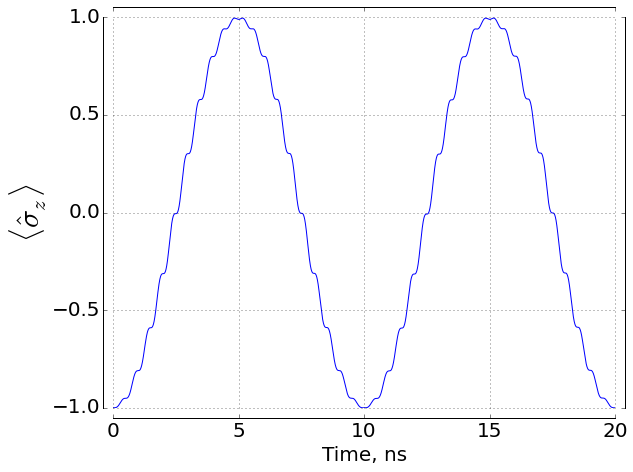
\includegraphics[height=0.225\textheight]{Pictures/rabi_dynamics_sz}
\end{subfigure}
\begin{subfigure}[t]{0.4\textwidth}
\centering
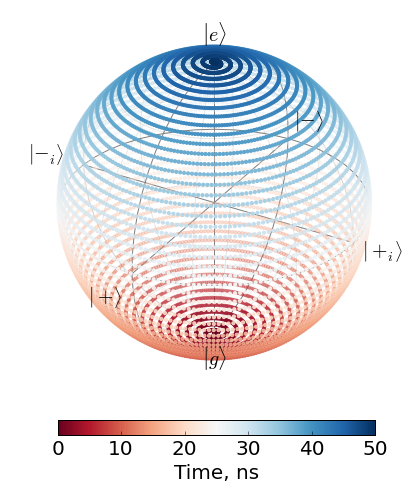
\includegraphics[height=0.225\textheight]{Pictures/rabi_dynamics_bloch2}
\caption{Динамика состояния кубита при подаче $\pi$-импульса.}
\end{subfigure}\quad
\begin{subfigure}[t]{0.5\textwidth}
\centering
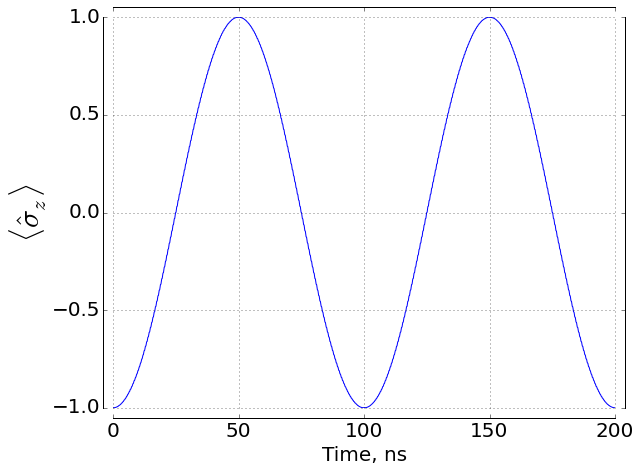
\includegraphics[height=0.225\textheight]{Pictures/rabi_dynamics_sz2}
\caption{Почти гармонические осцилляции $\left< \hat\sigma_z \right>$ за два периода.}
\end{subfigure}

\vspace{1cm}
\begin{subfigure}[t]{0.4\textwidth}
\centering
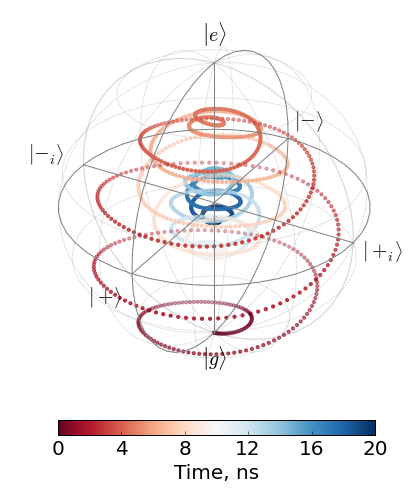
\includegraphics[height=0.225\textheight]{Pictures/rabi_dynamics_bloch_rel}
\caption{Релаксация затягивает кубит в центр сферы Блоха.}
\end{subfigure}\quad
\begin{subfigure}[t]{0.5\textwidth}
\centering
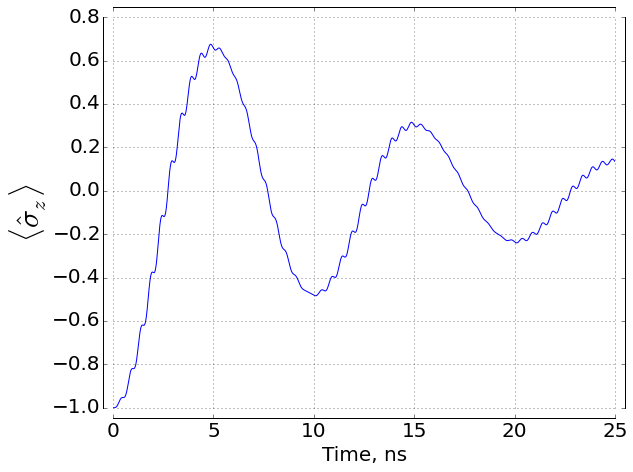
\includegraphics[height=0.225\textheight]{Pictures/rabi_dynamics_sz_rel}
\caption{Затухающие осцилляции $\left< \hat\sigma_z \right>$. Время затухания $\tau\approx1/\gamma = 10$ нс.}
\end{subfigure}
\caption{Кубит, вынуждаемый внешним гармоническим полем. $\omega/2\pi = \nu_q = 1$ ГГц, $A$=0.2 ГГц для верхней и нижней пар рисунков, $A$=0.02 ГГц для средней. Для нижней также $\gamma = 0.1$ ГГц. ``Рябь'' на графиках -- влияние слагаемых, которыми пренебрегают в RWA.}
\label{fig:rabi_osc}
\end{figure}


На \autoref{fig:rabi_osc}~(c,d) представлено затухание Раби-осцилляций, вызванное наличием релаксации. Характерное время затухания для не очень сильного вынуждения составляет порядка $1/\gamma$. Релаксация и вынужденное поглощение являются конкурирующими процессами, поэтому с течением времени кубит оказывается в равновесной области. Эта конечная область зависит от амплитуды возмущения: при сильном возмущении кубит в конце концов оказывается в окрестности центры сферы Блоха, а при слабом -- в области между центром сферы и основным состоянием.

\newpage

\section{Кубит, связанный с квантовым гармоническим осциллятором}

В данной работе исследовались потоковые кубиты, связанные с микроволновыми копланарными резонаторами, работающими в квантовом пределе. Связь возникает, когда магнитное поле стоячей волны резонатора создает сколько-нибудь заметный магнитный поток через кольцо кубита, и, тем самым, зависит от взаимной индуктивности этих двух объектов. Наличие связи качественно меняет поведение и кубита, и резонатора, и позволяет наблюдать целую плеяду новых эффектов.

\subsection{Гамильтониан Раби}

Самой простой моделью, описывающей взаимодействие кубита с резонатором, является \textit{модель Раби}. Так же, как, например, в теории взаимодействия атома со светом, гамильтониан невзаимодействующих частей дополняется оператором взаимодействия. В случае потокового кубита его нужно записать как $\mathcal{\hat H}_{int} = \hbar g\ \mathbf{\hat H}_{res} \otimes \hat \sigma_x = \hbar g\ (\hat a + \hat a^{\dag})\otimes \hat \sigma_x$, где $\mathbf{\hat H}_{res}$ -- проквантованное магнитное поле в резонаторе, а $g$ -- коэффициент перевода поля в поток, а затем в $\varepsilon$ из уравнения \eqref{eq:trunc_hamiltonian}. В итоге, получаем следующий модельный гамильтониан:
\begin{equation}
\begin{gathered}
	\mathcal{\hat H}_R = \hat{\mathcal{H}}_{q}+\hat{\mathcal{H}}_{r}+\hat{\mathcal{H}}_{i} \\
	\hat{\mathcal{H}}_{q} = \mathbbm{\hat 1}_r \otimes \hbar\left[\frac{\Delta}{2} \hat \sigma_z + 				\frac{\varepsilon}{2} \hat \sigma_x \right], \quad
	\hat{\mathcal{H}}_{r} = \hbar \omega_r \left(\frac{1}{2}+\hat a^\dag \hat a \right) \otimes \mathbbm{\hat 1}_q, \quad \\
	\hat{\mathcal{H}}_i = \hbar g (\hat a^\dag + \hat a) \otimes \hat \sigma_x
\end{gathered}
\label{eq:rabi_hamiltonian}
\end{equation}

Несмотря на свою простоту, СУШ для такого гамильтониана не имеет аналитического решения\cite{braak2011}. В связи с этим можно либо рассматривать приближения, либо решать задачу на собственные значения и векторы численно в матричной форме, ограничиваясь $N$ состояниями резонатора.

\begin{figure}

\begingroup
\captionsetup[subfigure]{justification=normal, width=0.8\textwidth}
\centering
\begin{subfigure}[t]{0.54\textwidth}
\centering
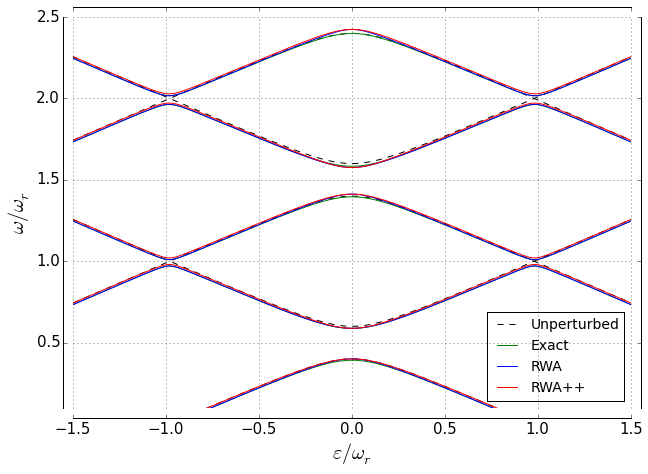
\includegraphics[scale=0.35]{Pictures/rabi_spectrum}
\caption{Спектр в зависимости от $\varepsilon$ для трех возможных приближений и для невзаимодействующей системы.}
\end{subfigure}
\begin{subfigure}[t]{0.44\textwidth}
\centering
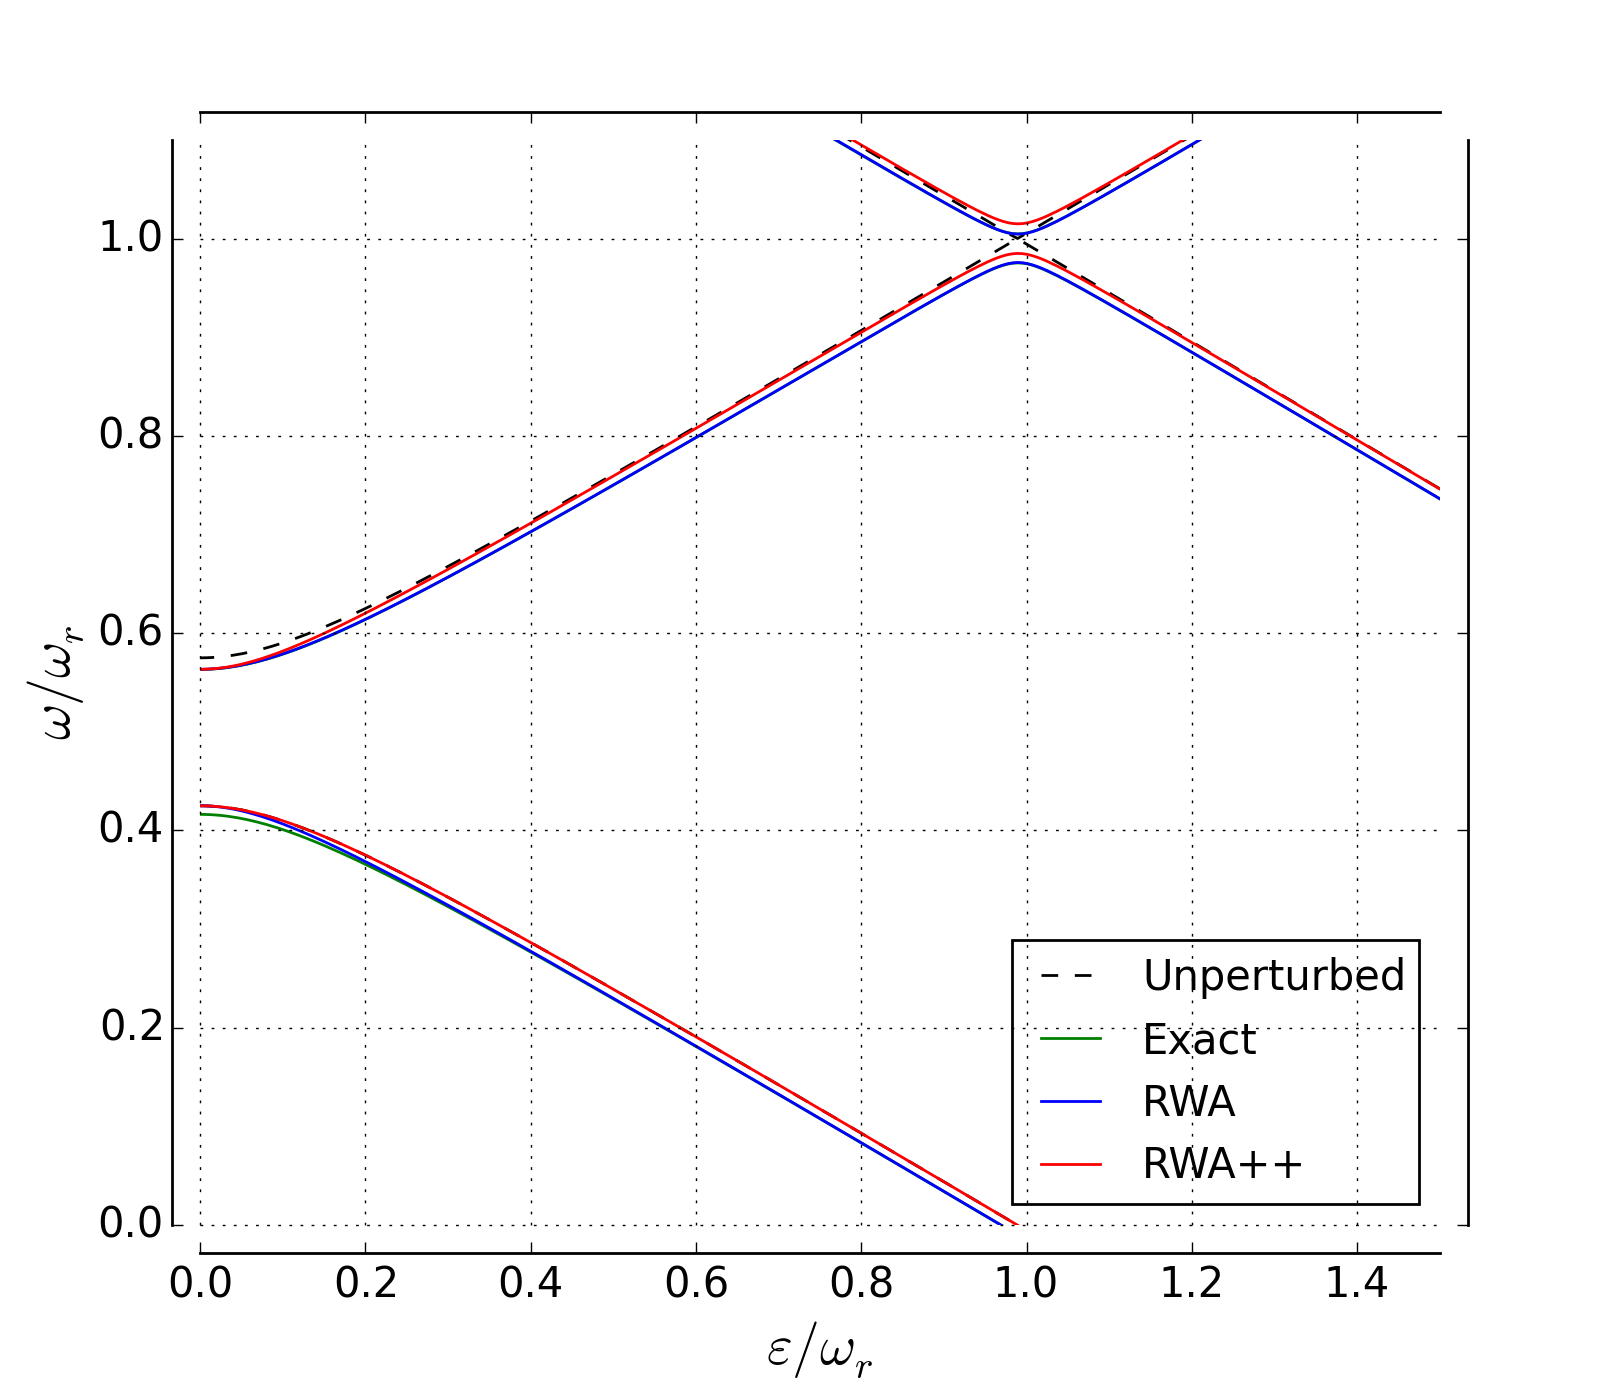
\includegraphics[scale=0.35]{Pictures/rabi_spectrum_closeup}
\caption{Увеличенная нижняя правая часть \textbf{(а)}, видны отклонения результатов друг от друга.}
\end{subfigure}

\vspace{1cm}

\captionsetup[subfigure]{width=0.9\textwidth}
\begin{subfigure}[t]{\textwidth}
\centering
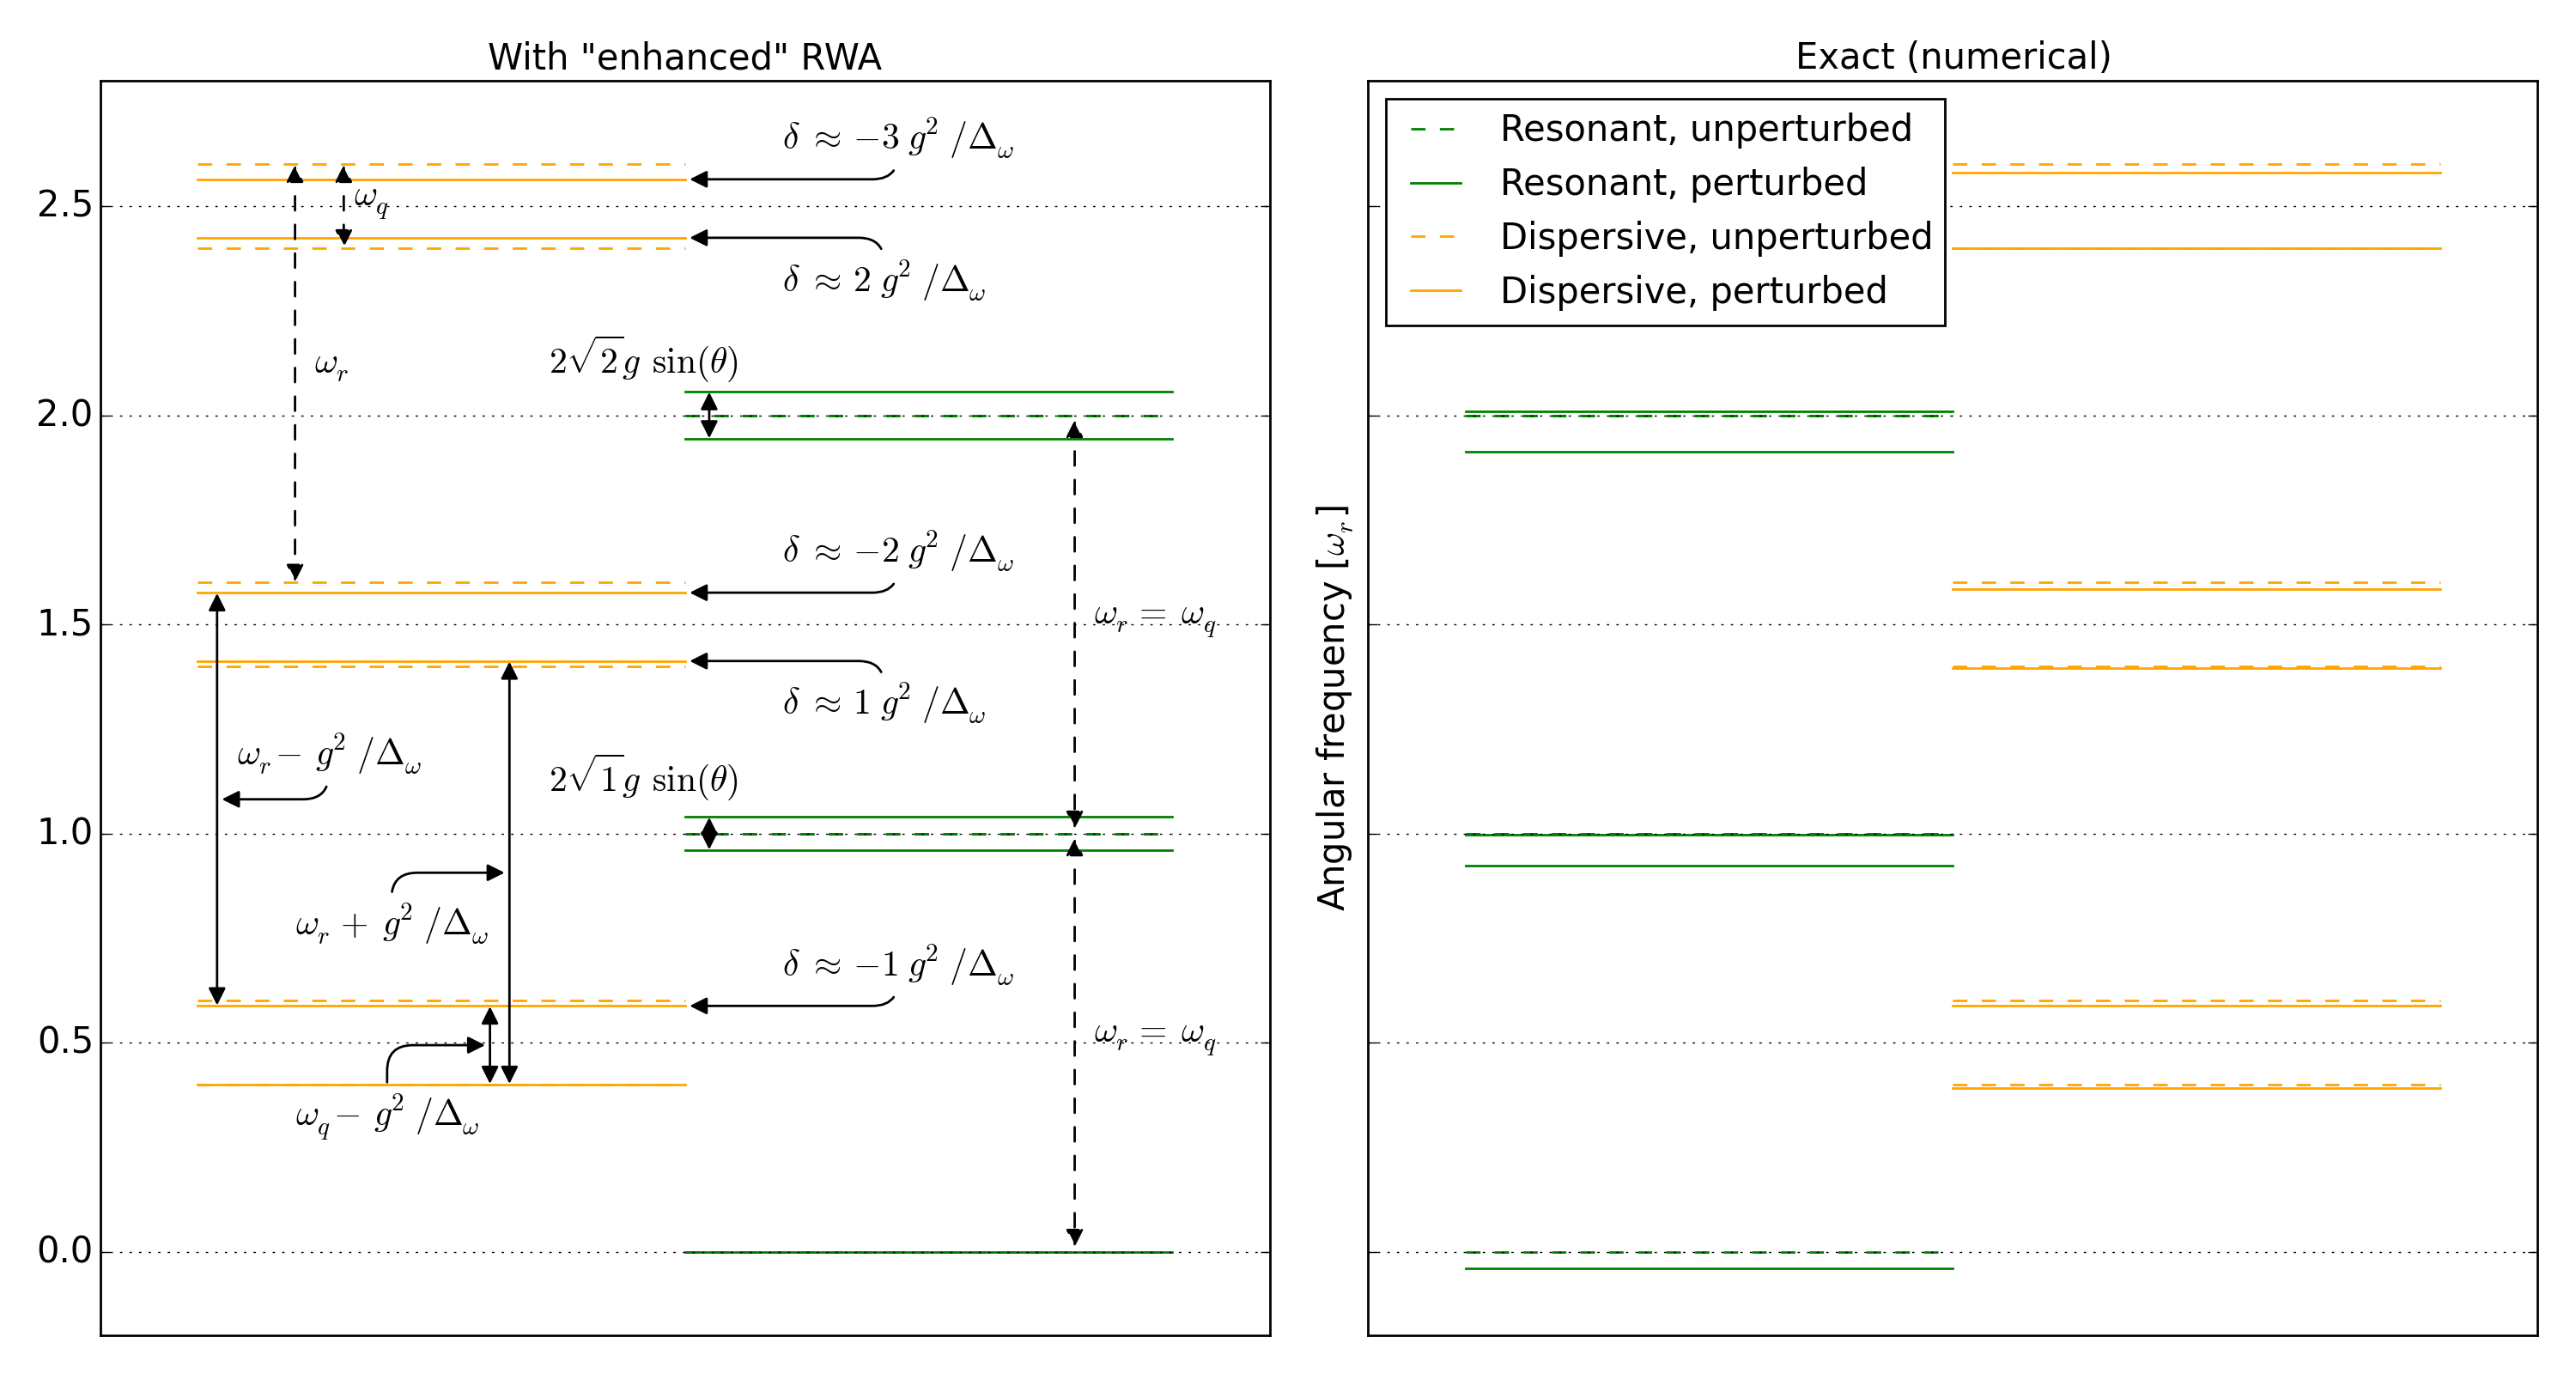
\includegraphics[width=.95\textwidth]{Pictures/JCM_levels}
\caption{Спектр в двух предельных случаях для точного решения и приближенного, для которого указаны аналитически полученные частоты. Для дисперсионного и резонансного режимов $\varepsilon = 0$ и $\varepsilon \approx 0.98\,\omega_r$ соответственно. Также для наглядности были использованы $g = 0.1\, \omega_r$ в дисперсионном и $g = 0.2\, \omega_r$ в резонансном режиме. $\Delta_\omega = |\omega_r - \omega_q| = \omega_r - \Delta$ при $\varepsilon = 0$}
\label{fig:rabi_analytic_spectrum}
\end{subfigure}
\caption{Подробный анализ спектра модели Раби и часто используемых приближений. $\Delta = 0.2\,\omega_r,\ g = 0.1\,\omega_r$}
\label{fig:rabi_spectrum}
\endgroup
\end{figure}

\subsection{Спектр модели Раби} \label{subsec:rabi_specrum}

Энергетический спектр гамильтониана \eqref{eq:rabi_hamiltonian} подробно рассмотрен на \autoref{fig:rabi_spectrum}. Большое внимание уделено часто используемому приближению RWA. Как ранее говорилось, приближения нужны, чтобы получить хотя бы какое-то аналитическое решение, однако важно понимать, когда их можно использовать и когда они перестают соответствовать действительности\cite{niemczyk2010, forn2010}. Для \eqref{eq:rabi_hamiltonian} перехода к RWA, допускающему решение (далее, ``улучшенный RWA''), требуется три шага:
\begin{enumerate}
\item \label{itm:first} Прежде всего нужно перейти к энергетическому представлению кубита. Для этого применяется оператор перехода $\mathcal{\hat U} = e^{i\frac{\theta}{2}\hat \sigma_y}$, где $\tg \theta = \varepsilon/\Delta$. Тогда $\hat{\mathcal{H}}_{q}$ и $\hat{\mathcal{H}}_{r}$ оказываются диагональными, а $\mathcal{\hat H}_i \rightarrow \hbar g (\hat a^\dag + \hat a) \otimes \left( \hat \sigma_x \sin\theta - \hat\sigma_z \cos\theta \right)$.

\item $\mathcal{\hat H}_i = \hbar g (\hat a^\dag + \hat a) \otimes \left( \hat \sigma_x \sin\theta-  \hat\sigma_z \cos\theta \right) \Rightarrow \hbar g \sin\theta \left(\hat a^\dag \otimes \hat \sigma^- + \hat a \otimes \hat \sigma^+\right) - \hbar g\cos\theta (\hat a^\dag + \hat a) \otimes \hat\sigma_z $ -- это стандартный прием RWA. Оправдать пренебрежение членами $\propto \hat a \otimes \hat \sigma^-, \hat a^{\dag} \otimes \hat \sigma^+$ можно \textit{только в резонансном случае и при малом g}, когда в невозмущенной задаче уровни близки к вырождению или вырождены, при помощи стационарной теории возмущений.

\item $\mathcal{\hat H}_i =\hbar g \sin\theta \left(\hat a^\dag \otimes \hat \sigma^- + \hat a \otimes \hat \sigma^+\right) -\hbar g\cos\theta (\hat a^\dag + \hat a) \otimes \hat\sigma_z \Rightarrow  \hbar g \sin\theta \left(\hat a^\dag \otimes \hat \sigma^- + \hat a \otimes \hat \sigma^+\right)$  -- ``улучшенный'' RWA, допускающий аналитическое решение. Пренебрежение вторым слагаемым можно оправдать опять же в рамках стационарной теории возмущений: окажется, что его эффект в резонансной области сводится к сдвигу уровней вверх (см. \autoref{fig:rabi_spectrum}~(b)). В точке вырождения этот член равен нулю сам по себе, поэтому в итоге, из непрерывности, частоты поглощения практически совпадают со стандартным RWA (см. \autoref{fig:rabi_freq_spectrum})
\end{enumerate}
\begin{figure}[h!]
\centering
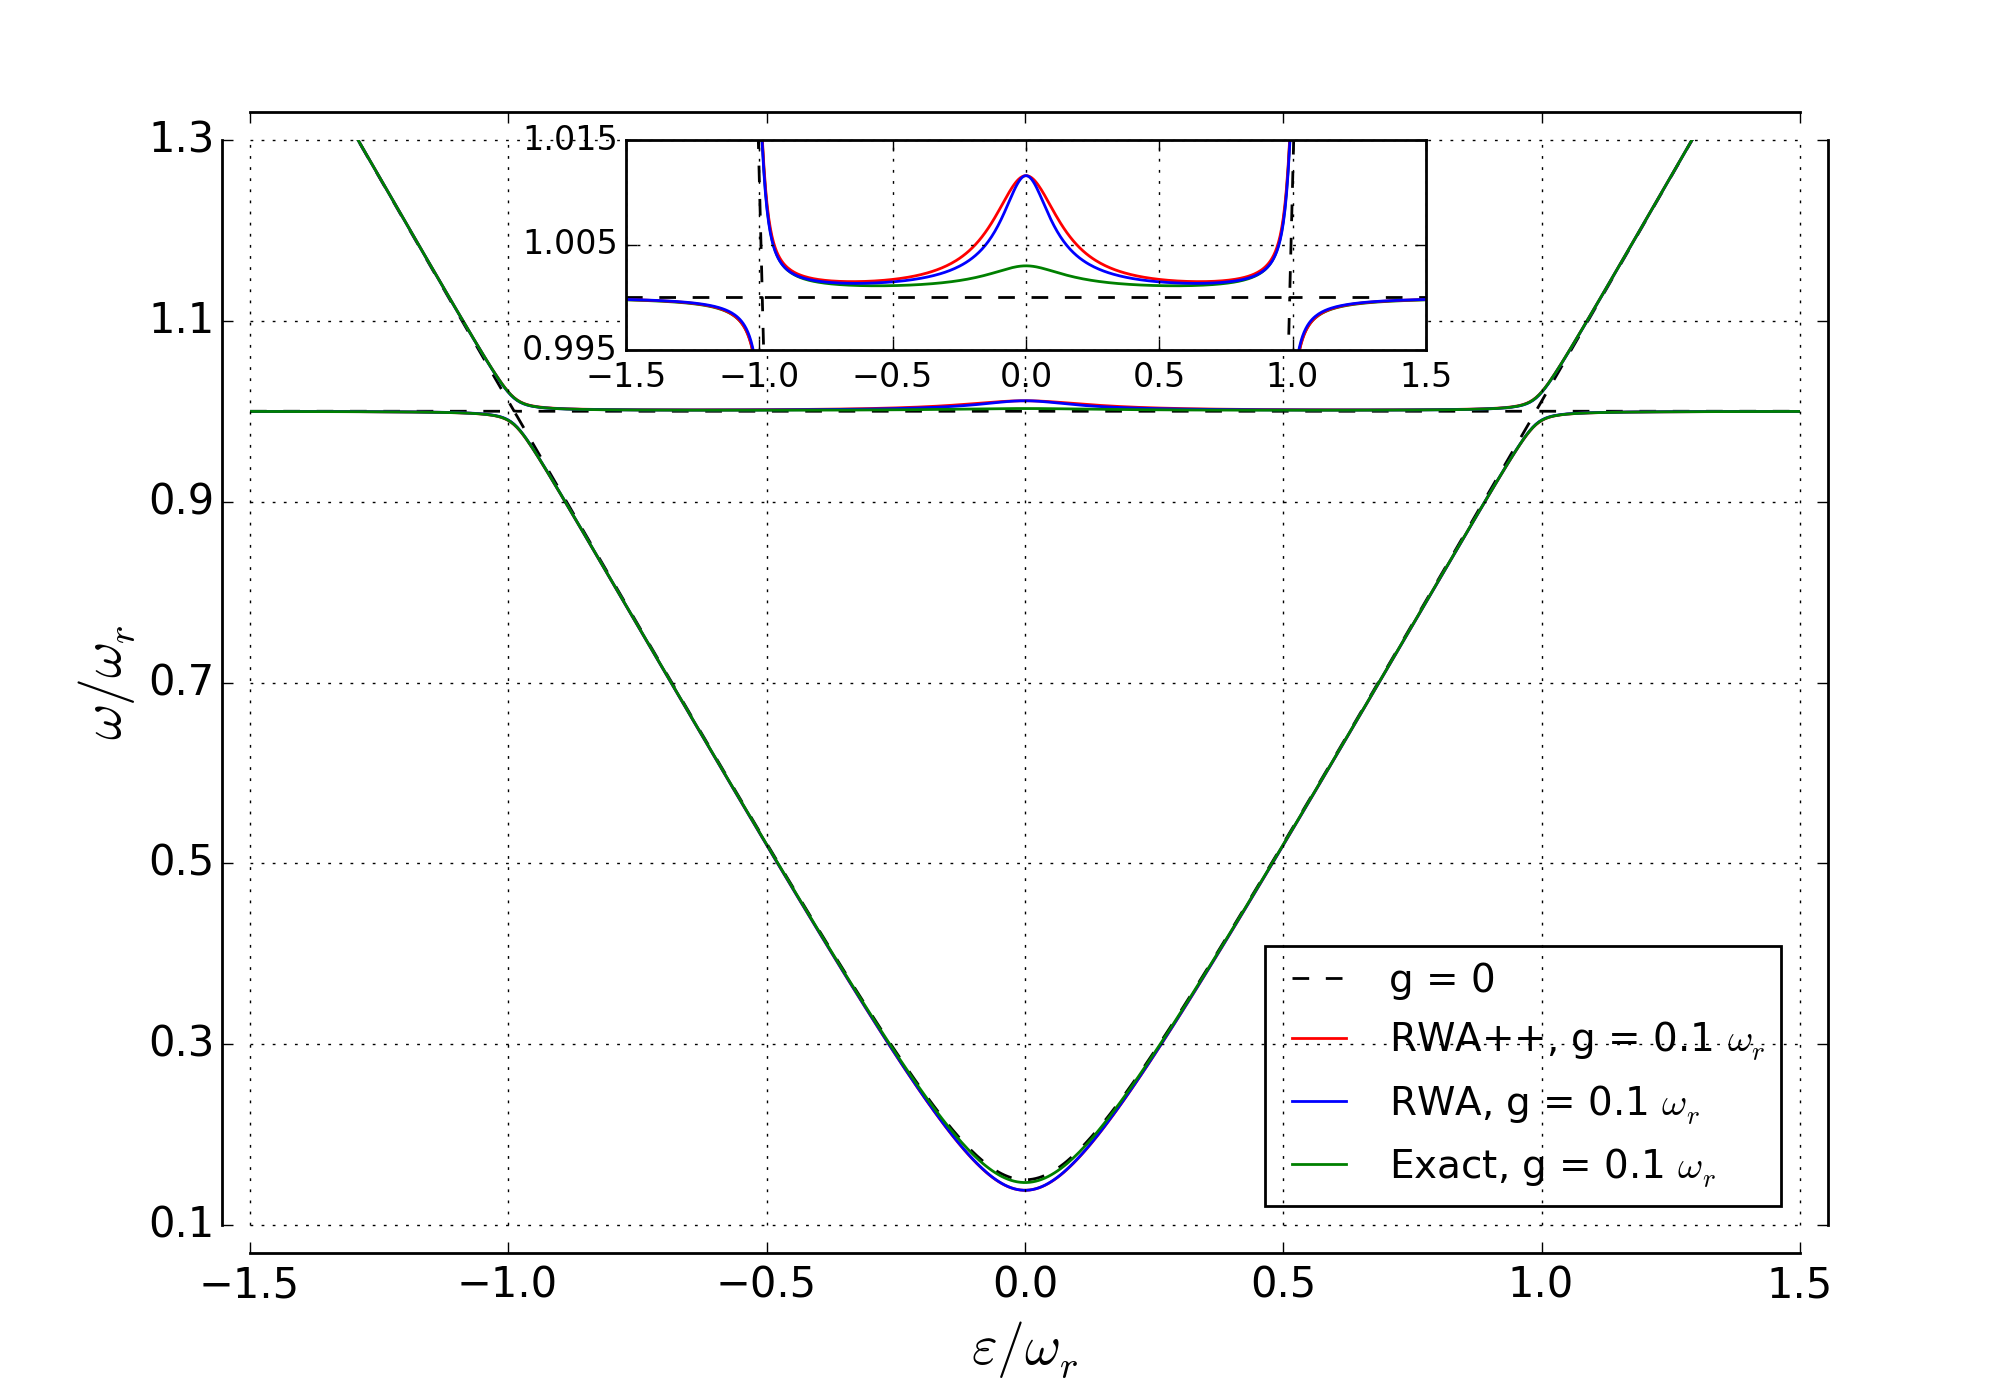
\includegraphics[width=0.8\textwidth]{Pictures/rabi_spectrum_freq}
\caption{Частотный спектр модели Раби для всех вариантов гамильтониана. Изображены переходы $\ket{0}\rightarrow\ket{1}$ и $\ket{0}\rightarrow\ket{2}$. На вставке: увеличенная окрестность $\omega_r$ по частоте.}
\label{fig:rabi_freq_spectrum}
\end{figure}


В итоге получаем аналитически разрешимый гамильтониан\cite{Jerger2013}, из которого рассчитаны выражения для сдвигов частот на \autoref{fig:rabi_spectrum}~(c). На \autoref{fig:rabi_freq_spectrum}, \autoref{fig:rabi_spectrum} видны так называемые \textit{квазипересечения} как уровней, так и частот там, где без $\mathcal{\hat H}_i$ наблюдалось бы вырождение состояний. Такое явление иногда представляется как критерий квантовомеханичекого поведения системы, однако квазипересечения есть и в классике\cite{novotny2010}. 


\newpage
\subsection{Динамика модели Раби} \label{subsec:rabi_specrum_dyn}

\begin{wrapfigure}[15]{r}{0.55\textwidth}
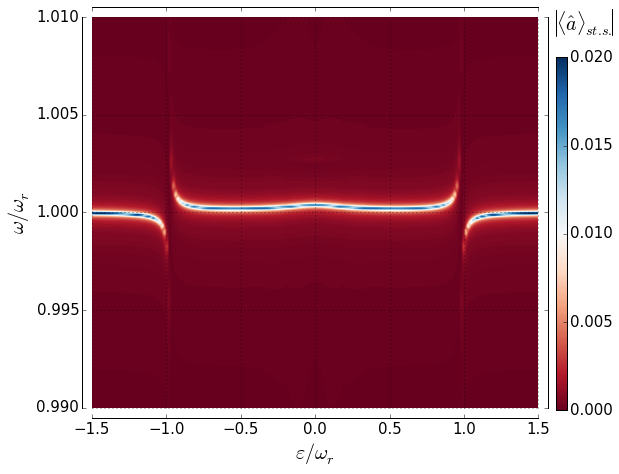
\includegraphics[width=0.5\textwidth]{Pictures/Rabi_anticrossing_far_dyn}
\caption{Симуляция динамического отклика модели Раби \eqref{eq:master_equation}. Параметры: $\kappa = 5\cdot 10^{-4}$, $\gamma = 0.01$, $\gamma_\phi = 0.007$, $\Delta = 0.2\,\omega_r$, $g=0.03\,\omega_r$}
\label{fig:rabi_spec_dyn}
\end{wrapfigure}

Для рассмотрения временнóго поведения связанной системы нужно использовать опять же основное уравнение. При наличии диссипации возникает вопрос о том, как записать диссипативные слагаемые: в пределе слабой связи выбирается просто сумма диссипаторов от кубита и от резонатора, однако, естественно, это приводит к проблемам в случае сильной связи\cite{beaudoin2011}. Далее мы тем не менее будем придерживаться простого вида диссипативной части:
\begin{gather*}
\mathcal{L}_{qr} \hat \rho = \kappa \mathcal{D}[\hat a \otimes \mathbbm{\hat 1}_q]\hat\rho + \\ +\gamma_\phi \mathcal{D}[\mathbbm{\hat 1}_r \otimes \hat \sigma_z]\hat\rho + \gamma\mathcal{D}[\mathbbm{\hat 1}_r \otimes \hat \sigma^-]\hat\rho .
\end{gather*}

Далее, рассмотрим модель взаимодействия системы с внешним электромагнитным полем. Для кубита остаются в силе рассуждения из \autoref{subsec:driven_qubit}, в то время как для резонатора нужно ввести новый формализм.	Для классического осциллятора, вынуждаемого внешней силой, можно записать следующее уравнение движения и его лагранжиан: 
$$m \ddot{x} + k x = F(t) \Leftrightarrow \mathcal{L} = \frac{m \dot{x}^{2}}{2}-\frac{kx^2}{2} + F(t) x .$$
Переходя к гамильтониану, производя каноническое квантование и переход к представлению чисел заполнения для осциллятора, получаем вид оператора, отвечающего за действие вынуждающей силы:
\[
\mathcal{\hat V}_r = -\frac{\hbar F(t)}{\sqrt{2\hbar m \omega_0}} (\hat a + \hat a^{\dag}) \overset{def}{=} - \hbar f_r (\hat a + \hat a^{\dag}) \sin \omega t.
\label{eq:osc_driving_term}
\]
Таким образом, мы имеем все части линдбладовского уравнения, который описывает эволюцию системы кубит-резонатор. Выпишем его в явном виде (важно осуществить переход к энергетическому представлению кубита\cite{ithier2005}):
\begin{gather}
\frac{\partial}{\partial t} \hat \rho= \frac{i}{\hbar}\left[\hat \rho, \mathcal{\hat H}_R^\prime \right] + \mathcal{L}_{qr}\hat \rho, 
\label{eq:master_equation}
\\
\mathcal{\hat H}_R^\prime = \mathbbm{\hat 1}_r \otimes \frac{\hbar \omega_q}{2} \hat \sigma_z  + \hbar \omega_r \left(½ +\hat a^\dag \hat a \right)\otimes \mathbbm{\hat 1}_q + \hbar g (\hat a^\dag + \hat a) \otimes \left( \hat \sigma_x \sin\theta-  \hat\sigma_z \cos\theta \right) + \notag
\\ 
+\hbar f_q \cos(\omega t)~ \mathbbm{\hat 1}_r \otimes \left( \hat \sigma_x \sin\theta -  \hat\sigma_z \cos\theta \right) - \hbar f_r \cos(\omega t) (\hat a^\dag + \hat a)\otimes \mathbbm{\hat 1}_q ,  \notag
\end{gather}

\begin{wrapfigure}[16]{r}{0.5\textwidth}
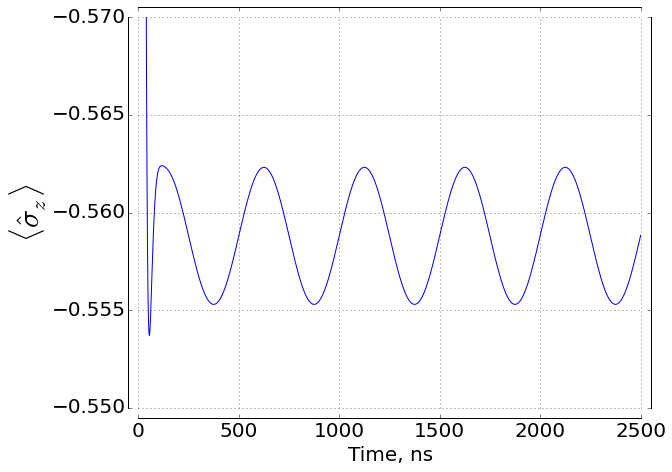
\includegraphics[width=0.5\textwidth]{Pictures/oscillatory_quasisteadystate}
\caption{Слабо осциллирующее поведение кубита при слабом вынуждении и наличии релаксации.}
\label{fig:oscillatory_ss}
\end{wrapfigure}

\hspace{-\parindent}где $f_q$ и $f_r$ -- эффективные энергетические амплитуды поля в области кубита и на входе резонатора, а $\mathcal{L}_{qr}$ определен выше. Уравнение \eqref{eq:master_equation} нужно решать численно, например, на конечном интервале времени. В случае моделирования спектроскопии решение заключается в обнаружении \textit{стабильного состояния} $\hat \rho_s$, т.е. такого что $\frac{\partial }{\partial t}\hat \rho_s = 0$, в котором система оказывается на больших временах эволюции. В связи с временнóй зависимостью $\mathcal{\hat H}_R^{\prime}$ с необходимостью $[\hat \rho_s, \mathcal{\hat V}_r + \mathcal{\hat V}_q] = 0$, а $[\hat \rho_s, \mathcal{\hat H}_R] = - \mathcal{L}_{qr}\hat\rho_s$. 
Если первое условие не выполнено, то можно либо говорить о почти стабильных слабо осциллирующих состояниях (\autoref{fig:oscillatory_ss}), где $\frac{\partial }{\partial t}\hat \rho_s \approx 0$, либо об отсутствии решения задачи. Для ускорения решения иногда применяется также переход во вращающийся базис\cite{Bishop2010}, где гамильтониан в приближении RWA (для внешнего поля, как и в \autoref{subsec:driven_qubit}) не зависит от времени, и стационарное состояние ищется как решение линейной системы.

\begin{figure}[h!]
\centering
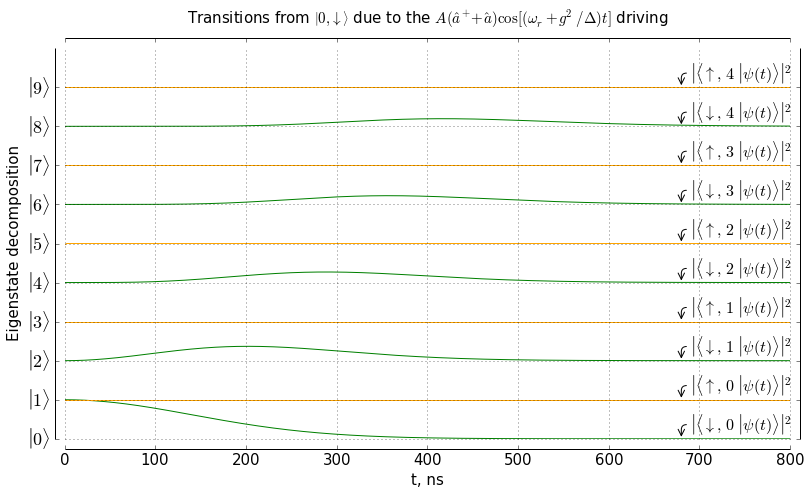
\includegraphics[width=0.7\textwidth]{Pictures/climbing}
\caption{Переходы под действием возмущения на дисперсионно сдвинутой частоте.}
\end{figure}

Руководствуясь соображениями, которые будут приведены в \autoref{subsec:input-output}, из стабильного решения уравнения \eqref{eq:master_equation} можно получить экспериментально наблюдаемый спектр системы. На \autoref{fig:rabi_spec_dyn} сразу видна явная особенность: мы можем видеть только часть спектра, предсказываемого стационарной моделью \eqref{eq:rabi_hamiltonian} (\autoref{fig:rabi_freq_spectrum})  в окрестности $\omega_r$. Связано это с тем, что в эксперименте во-первых, коэффициент $A\gg B$, так что оператор $\mathcal{\hat V}_q$ не играет роли, а $\mathcal{\hat V}_r$ не может возбудить кубит, так как матричный элемент перехода по ``кубитным'' состояниям $\ket{n, \downarrow},\ \ket{n, \uparrow}$ для него равен нулю. Поэтому в дисперсионном режиме при разумных $g$, когда собственные состояния приблизительно факторизованы, поглощения на частоте кубита нет\cite{Blais2004}. Вторая причина связана с тем, как моделируется отклик, и будет объяснена ниже.

\subsection{Теория отклика} \label{subsec:input-output}

При моделировании любого эксперимента необходимо понимать, что является наблюдаемой физической величиной. В экспериментальной части данной работы будет показано, что в эксперименте происходит \textit{гетеродинное детектирование} сигнала, исходящего от образца. Так как основное уравнение, которым до сих пор мы пользовались, описывает динамику внутри системы, но явно не дает информации о том, какое влияние она оказывает на внешнюю среду, необходимо применить дополнительный аппарат -- \textit{теорию отклика}\cite{Bishop2010, clerk2010, gardiner1985} (input-output theory). Идейно она похожа на ту, что была использована для получения диссипативной динамики подсистем, и заключается так же в записи полного гамильтониана для системы и для передающей линии, с которой она соединена слабой связью:
$$\mathcal{\hat H}_{tot} = \mathcal{\hat H}_{sys} +\int d\omega\ \hbar \omega \hat b^\dag(\omega) \hat b(\omega) + \int d\omega\ [ \kappa(\omega) \hat c^{\dag} \hat b(\omega) + \kappa(\omega)\hat c \hat b^{\dag}(\omega)],	$$ 
где $\hat c$ -- оператор, через который система связана с линией. Для такого гамильтониана выводятся уравнения движения Гейзенберга, и после определенных преобразований находится соотношение 
\begin{equation}
\hat b_{out} = \sqrt{\kappa}\hat c,
\label{eq:b_out}
\end{equation} 
связывающее исходящую амплитуду поля с некоторым оператором системы ($\kappa$ принята не зависящей от частоты). Выражение \eqref{eq:b_out} записано для линии с двумя интерфейсами: входом и выходом, причем драйв на входе учитывается членом $\mathcal{\hat V}_r$ в основном уравнении, а на выходе мы пренебрегаем прошедшим насквозь $\hat b_{in}$. Таким образом, оказывается, что основное уравнение все же дает информацию об излученной волне, причем для коэффициента прохождения при гетеродинном детектировании верно\cite{Bishop2010}
\begin{equation}
T \propto | \langle \hat a \otimes \mathbbm{\hat 1}_q \rangle_{s} | = |\Tr{\hat \rho_s \hat a }|.
\label{eq:transmission}
\end{equation}
В уравнении \eqref{eq:transmission} $\hat c$ был заменен на $\hat a \otimes \mathbbm{\hat 1}_q $, и эта наивная замена может приводить к парадоксам. К примеру, в случае сильной связи основное состояние имеет ненулевое среднее значение этого оператора, и по формуле \eqref{eq:transmission} должно демонстрировать некоторое конечное пропускание в любых условиях, затмевая полезные эффекты. Использование такой формулы также приводит к тому, что состояние кубита не дает вклада в пропускание, что заканчивает начатое в предыдущем разделе объяснение.


\chapter{Экспериментальная часть} \label{chap:exp}

Целью экспериментальной части работы была проверка совпадения теории с экспериментом и, так как многими группами было доказано блестящее их соответствие\cite{bishop2009, niemczyk2010, forn2010}, качества наших установки и образца. Второй целью было наблюдение зависимости расщепления Раби и сдвига Блоха-Сиджерта\cite{forn2010} (отклонения точного решения от приближения RWA) от фундаментального расщепления $\Delta$ кубита, так как на одном образце их было несколько. 

\section{Установка и оборудование}

Эксперимент проводился в Лаборатории сверхпроводящих метаматериалов НИТУ МИСиС. Лаборатория была создана в 2013 году и обладает оборудованием для получения низких температур, микроволновым оборудованием для измерения спектральных характеристик образцов, устройствами крепления образцов внутри криостата и подвода к ним микроволновых коаксиальных кабелей, пилой для обрезки чипов и множеством других полезных устройств. 

\subsection{Рефрижератор растворения}

Центральным прибором лаборатории является рефрижератор растворения, произведенный компанией Oxford Instruments. Это сложный инструмент, позволяющий получать температуры до 25 мК -- такая температура требуется во-первых для работы сверхпроводящей электроники, а во-вторых, что более важно, сводит на нет термальное шумовое возбуждение кубита. 

\paragraph{Общая характеристика.} Рефрижератор состоит из двух частей: компрессора c турбомолекулярным насосом, находящихся в подвале, и вакуумной камеры с постом управления внутри самой лаборатории. Компрессор служит для работы \textit{термоакустической криогенной системы} (pulse tube), а насос для откачки паров гелия-3.

Верхняя часть установки без поста управления изображена на \autoref{fig:fridge}~(a). Внутренняя часть изображена на \autoref{fig:fridge}~(b) и состоит из последовательно расположенных уровней (далее \textit{пластин}), каждый из которых достигает в охлажденном режиме своей температуры -- чем ниже уровень, тем она меньше. Для охлаждения требуется свести к минимуму теплообмен со средой, поэтому в криостате устроена система из четырех коаксиальных щитов, которые последовательно надеваются на подвес, а затем откачиваются турбовакуумным насосом. После охлаждения вакуум достигает $10^{-6}$ торр и обеспечивает хорошую термическую изоляцию.

Для коммуникации внутрь криостата подведены коаксиальные кабели для микроволновых сигналов (8 линий) и медные витые пары для постоянного тока (три линии, по 12 пар на каждой), что вкупе с довольно большим размером низшей пластины позволяет в принципе размещать несколько образцов на нескольких держателях.


\begin{figure}
\centering
\begingroup

\captionsetup[subfigure]{width = 0.9\textwidth, justification=normal}
\begin{subfigure}[t]{0.45\textwidth}
\centering
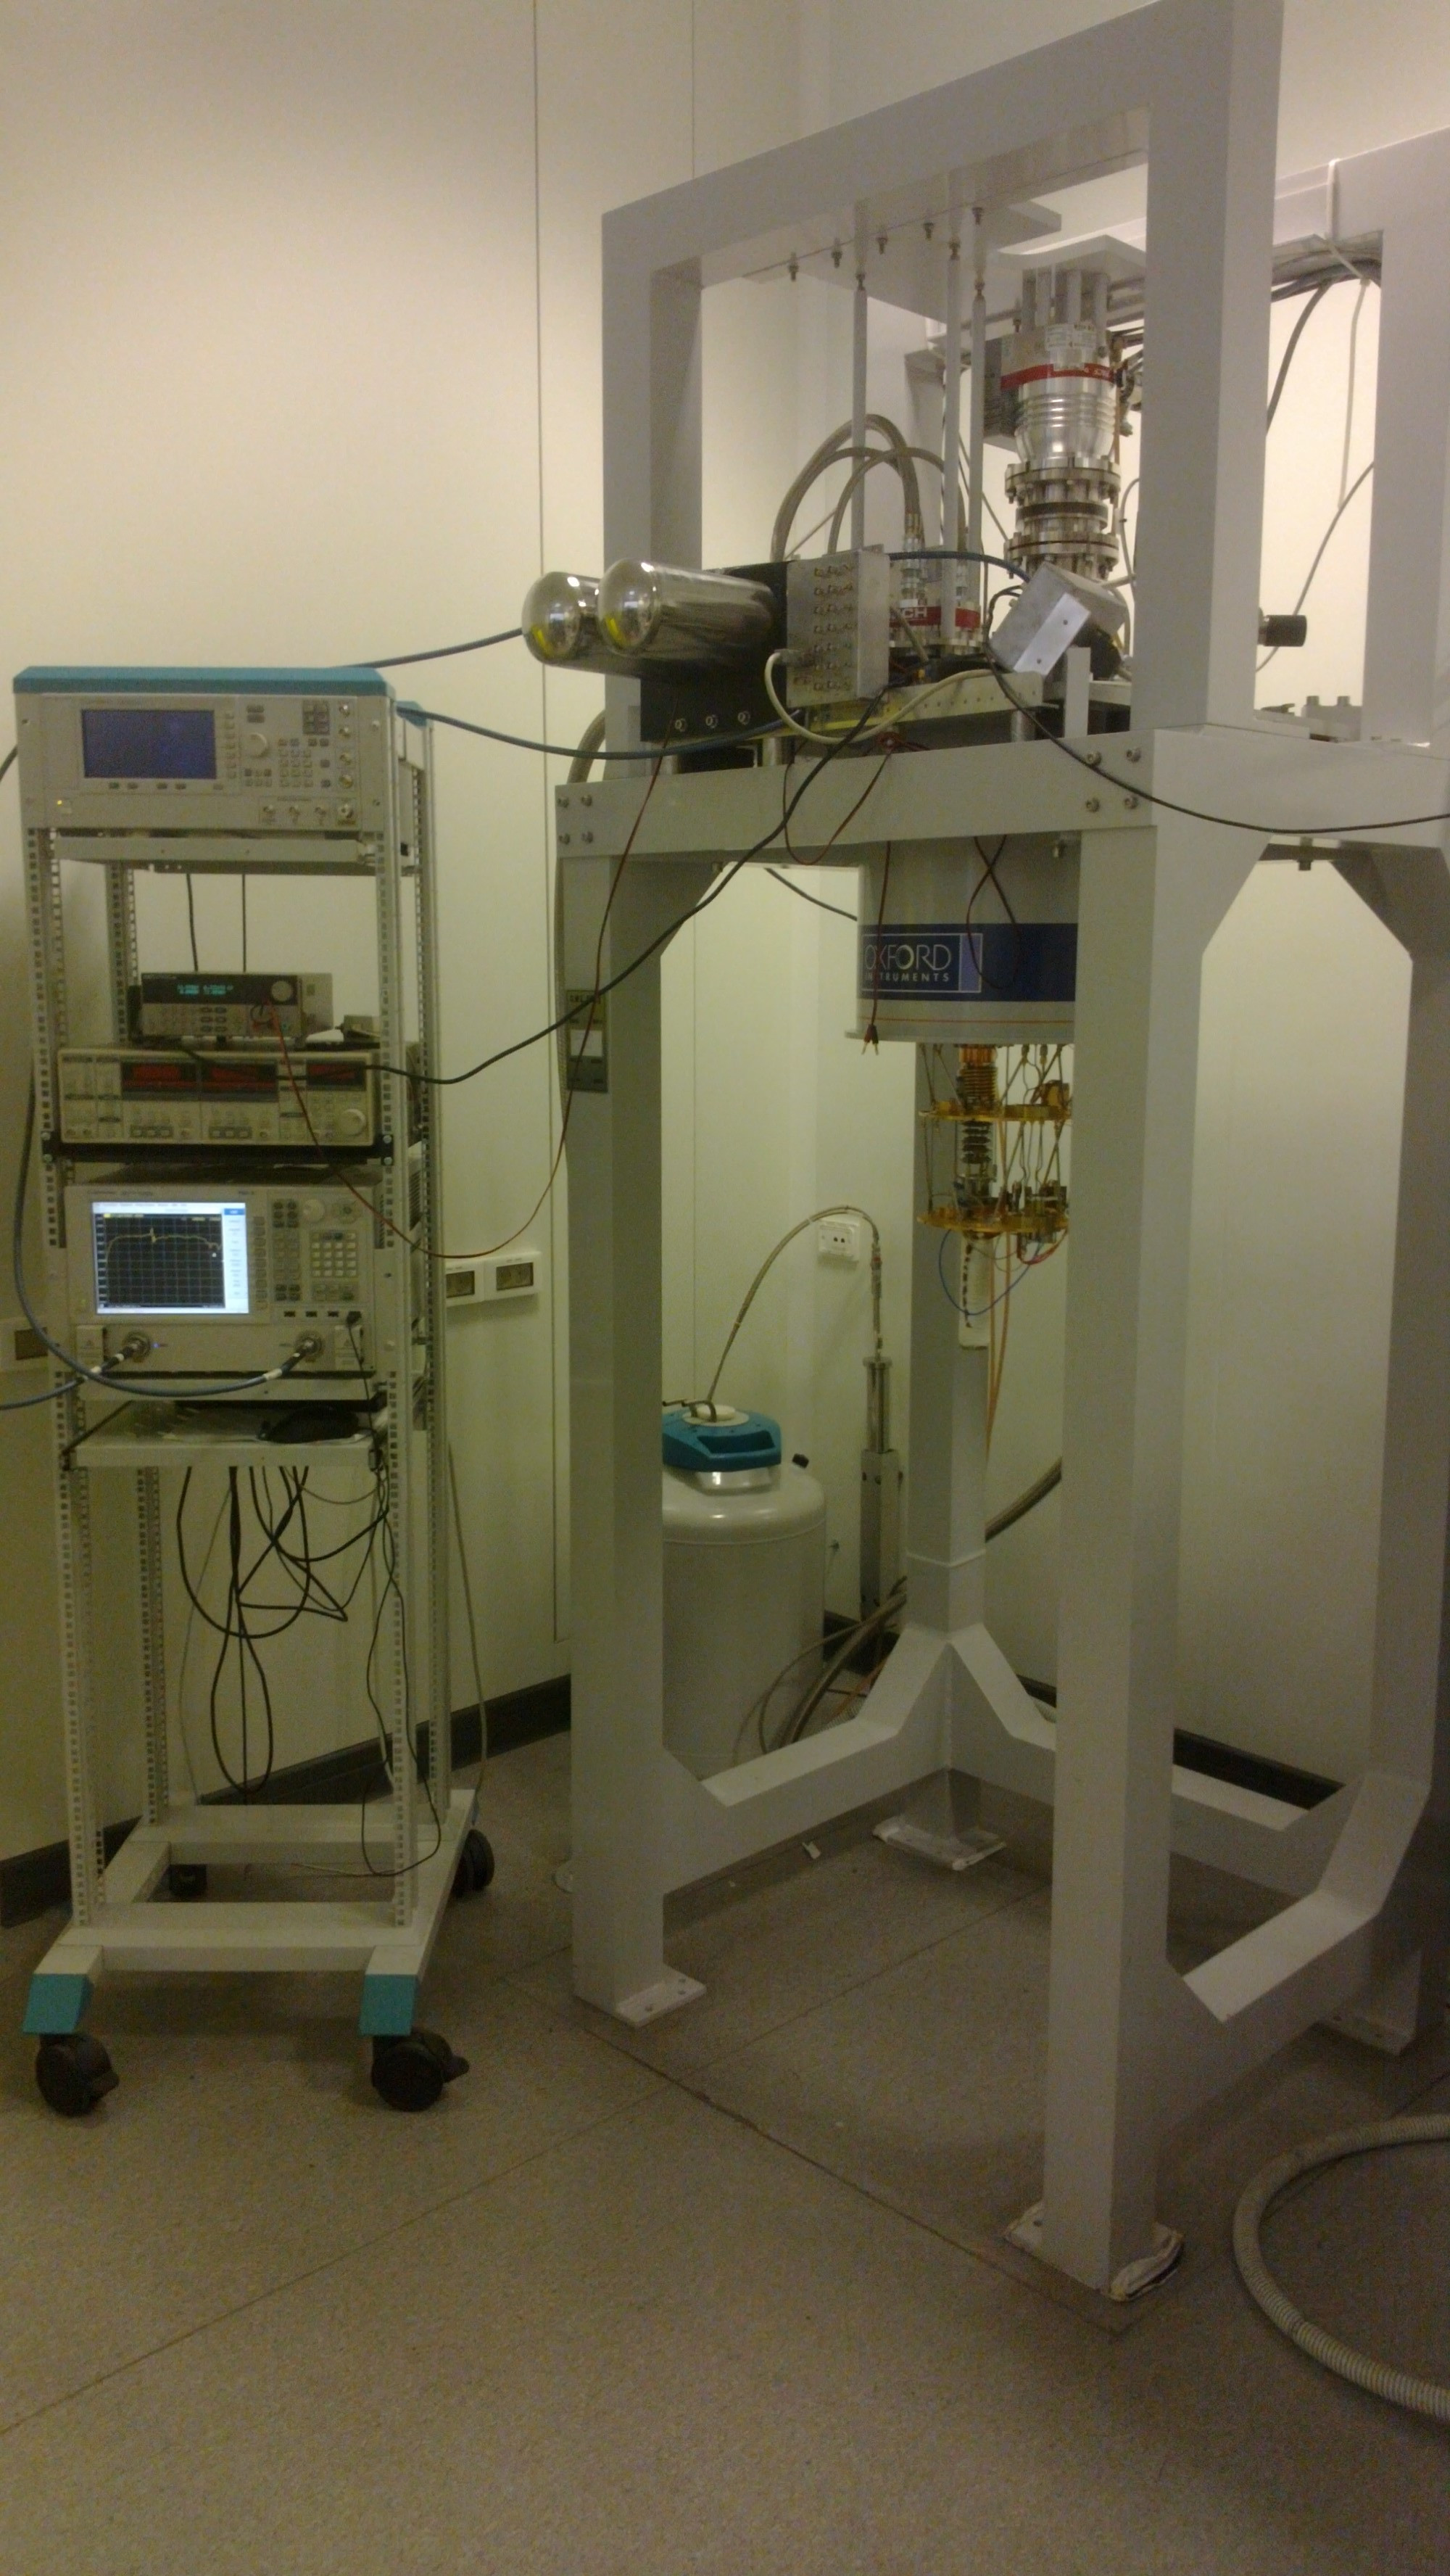
\includegraphics[height=0.4\textheight]{Pictures/cryo_general_view}
\caption{Общий вид верхней части фриджа. Видны пульсационная трубка (два цилиндра), вспомогательная турбина (цилиндр вверху) и внешний щит. Также присутствуют азотная ловушка и бак с азотом (внизу).}
\end{subfigure}
\begin{subfigure}[t]{0.45\textwidth}
\centering
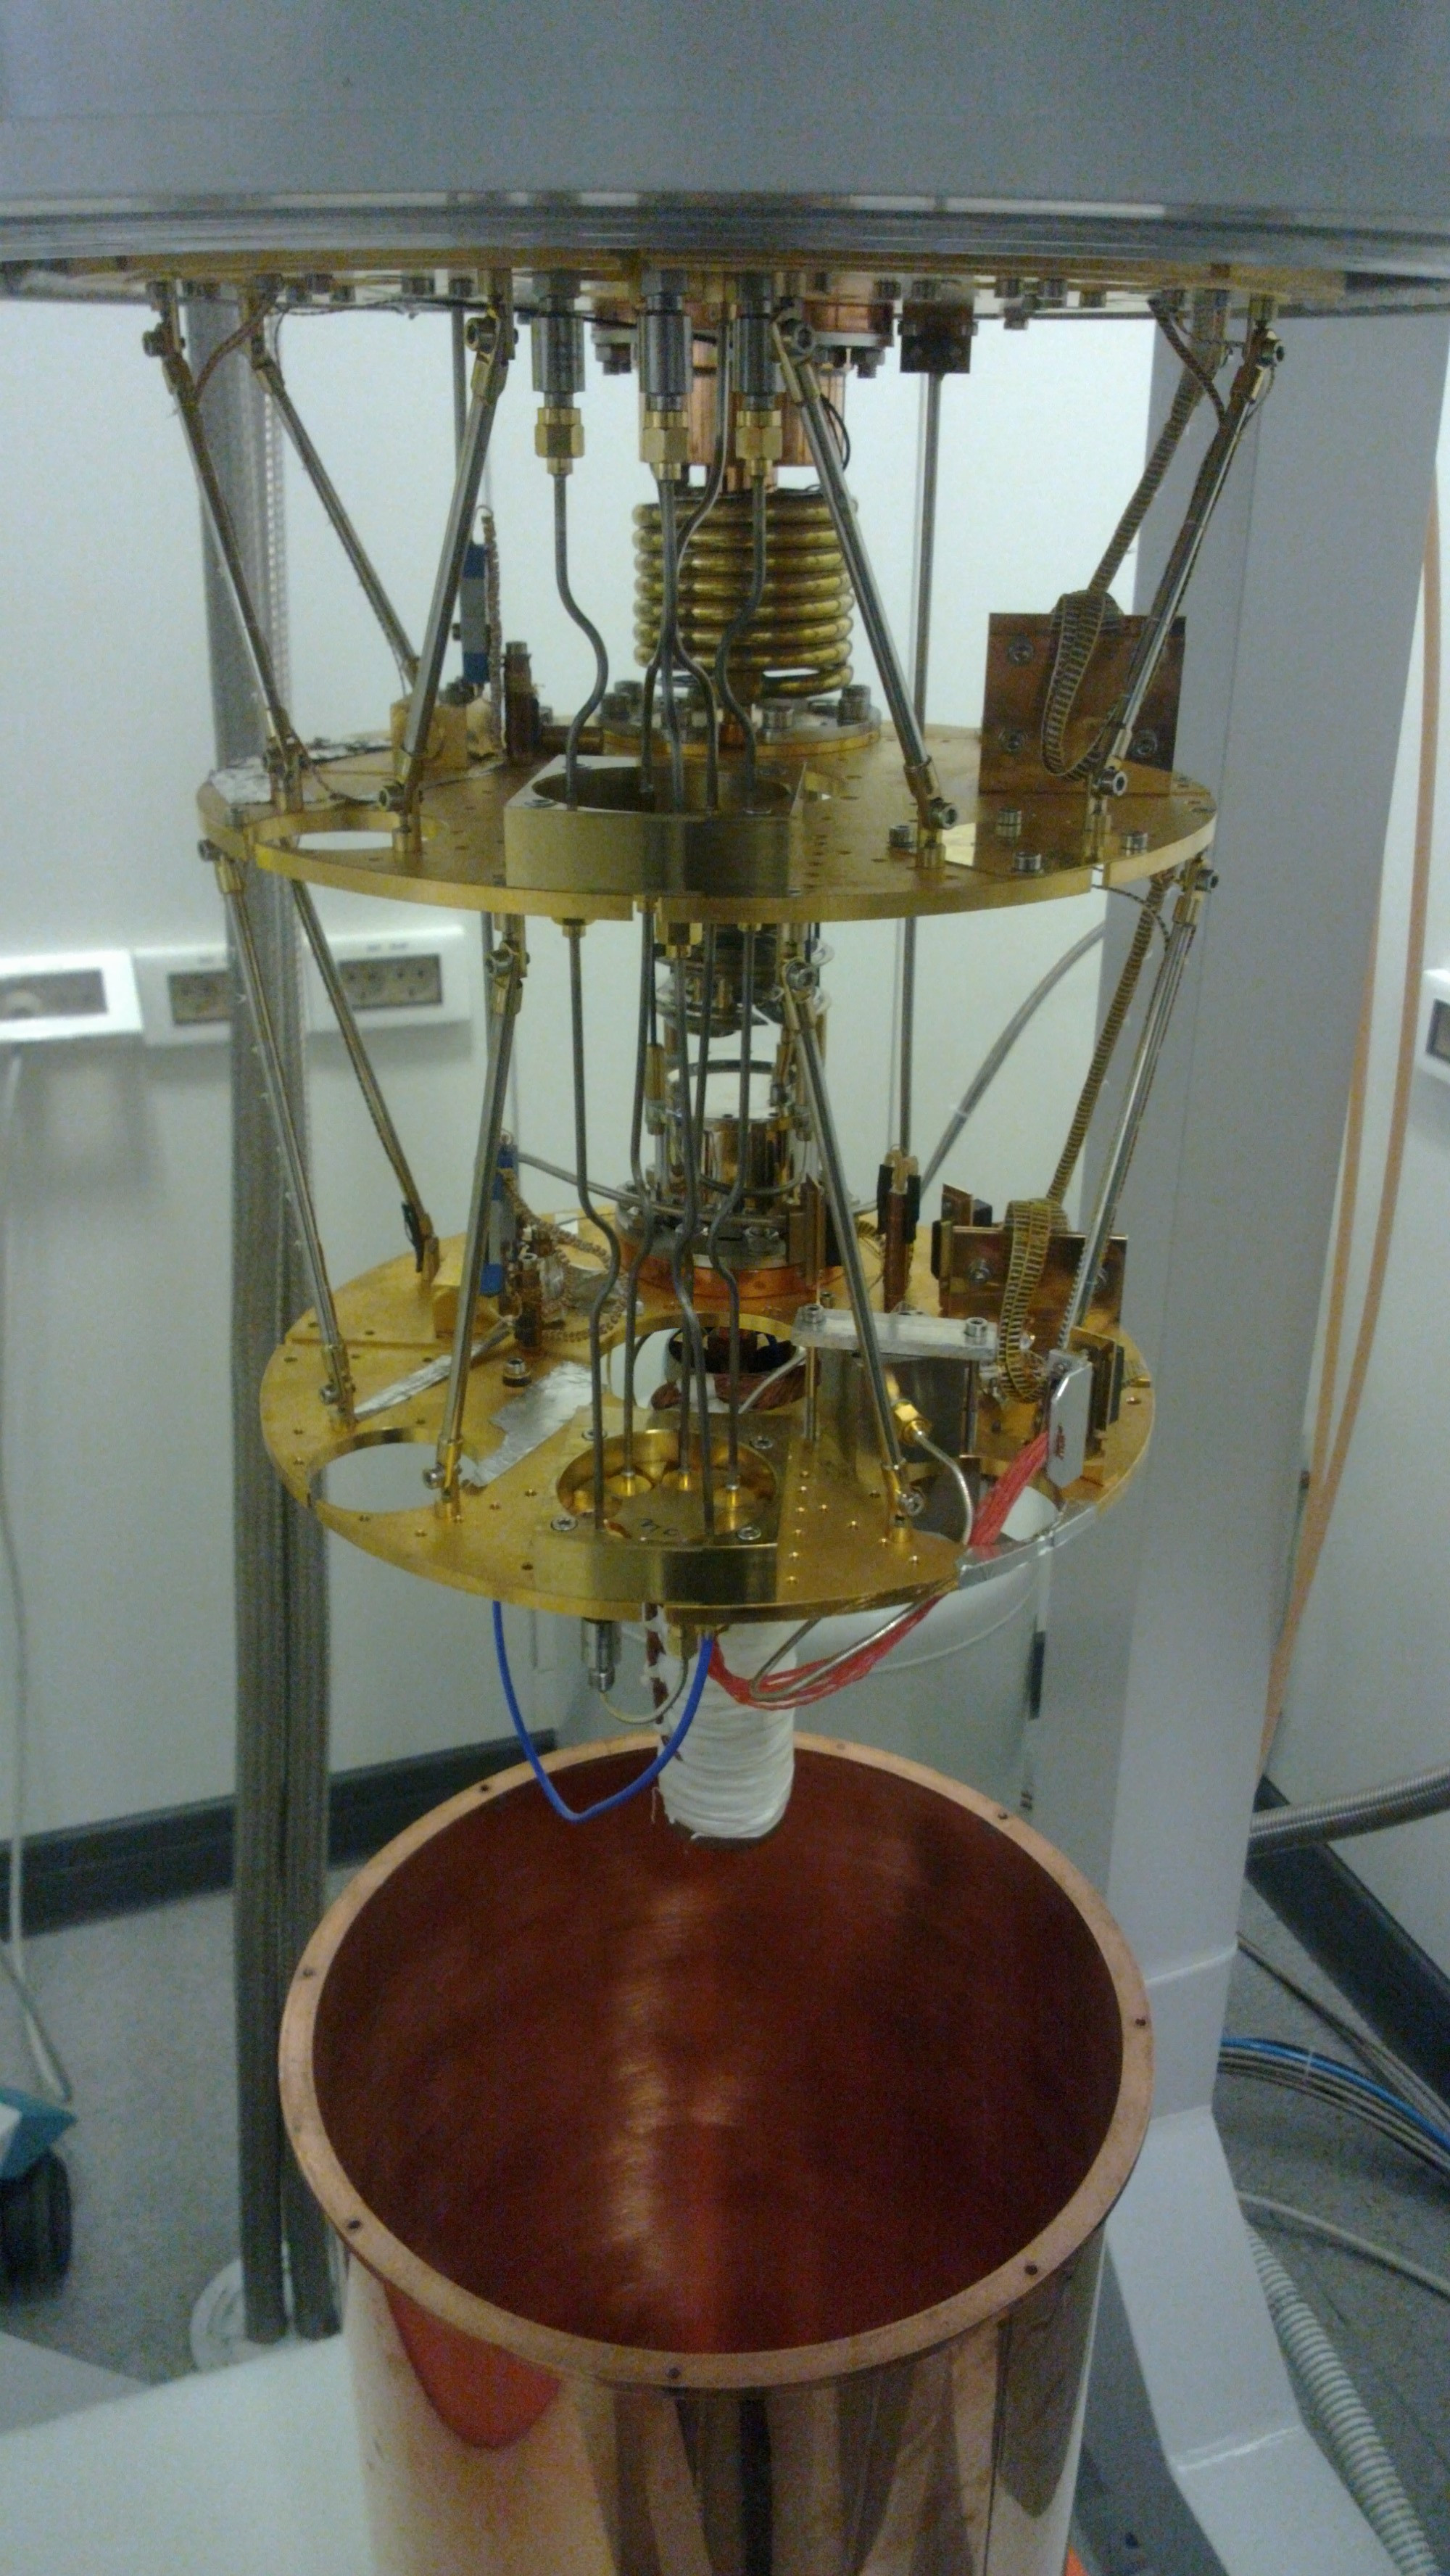
\includegraphics[height=0.4\textheight]{Pictures/cryo_inside}
\caption{Внутренняя часть установки. Видны две нижние пластины с коммуникациями, 100 мК и 25 мК, в последнюю снизу ввинчивается держатель образца. Также виден внутренний отражающий медный щит.}
\end{subfigure}
\endgroup
\caption{Общий вид охлаждающей установки, расположенной в лаборатории.}
\label{fig:fridge}
\end{figure}

\paragraph{Принцип работы.} Рефрижератор использует эффект абсорбции тепла при переходе $^3$He из однородной фазы в растворенную в $^4$He. Происходит этот процесс следющим образом: вначале происходит термоакустическое охлаждение смеси $^4$He -$^3$He и до $\approx 700$ мК, когда происходит самопроизвольное разделение изотопов на два слоя: чистый $^3$He, который оказывается сверху, и $^4$He под ним,  
\begin{wrapfigure}{r}{0.3\textwidth}
\begingroup
\captionsetup{justification=normal}
\centering
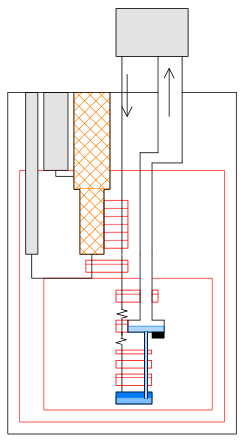
\includegraphics[width=0.25\textwidth]{Pictures/fridge_principle}
\caption{Схема контура охлаждения. Вверху слева: контур акустического охлаждения. Внизу и по центру: контур охлаждения смесью.}
\label{fig:fridge_principle}
\endgroup
\end{wrapfigure}
в котором, в силу некоторого превышения ван-дер-ваальсовского притяжения между атомами $^4$He и $^3$He над притяжением между атомами $^3$He, содержится около 6.6\% $^3$He (при 0 K).
Далее начинается откачка гелия-3, как показано на \autoref{fig:fridge_principle} (темно-синий -- $^3$He, голубой -- смесь $^4$He -$^3$He). В результате в камере смешения под действием осмотического давления происходит обеднение раствора $^4$He -$^3$He, которое компенсируется ``испарением'' гелия-3: он растворяется из верхнего слоя в нижний для поддержания постоянной при заданной температуре его концентрации ($\approx 6.6\%$ при низких T). При таком растворении происходит отбор тепла от камеры смешивания и всего окружения согласно следующему закону:
$$ \dot Q = T \dot \nu_3[s_3(x_l) - s_3(x_u)], $$
где $\dot \nu_3$ -- молярная скорость прокачки $^{3}$He, $s_3(x_{l, u})$ -- молярные энтропии $^{3}$He в зависимости от его концентрации $x_{l, u}$ в растворенной и чистой фазах соответственно, а $\dot Q$ -- мощность охлаждения. В итоге получаем замкнутый контур: гелий-3 циркулирует по системе, растворяясь, откачиваясь, и поступая обратно туда, откуда растворялся.
При выключении смесь собирается в специальный бак при помощи турбомолекулярного насоса и, дополнительно, специальной турбины, установленной в верхней части криостата. 


\subsection{Микроволновое оборудование}

Хотя в теории частоты кубитов могут быть практически любыми, в реальности они ограничены микроволновым диапазоном, так как при больших частотах излучение начинает испытывать фундаментальное поглощение в сверхпроводнике (например, в алюминии щель $\Delta \approx 3.4 \cdot 10^{-4}$ эВ  соответствует по частоте примерно 80 ГГц), что приводит к неприменимости использованных моделей. В силу этого в лабораториях, работающих с твердотельными кубитами, используются различные приборы микроволнового диапазона.

\paragraph{Векторный анализатор цепей.} Этот прибор используется для определения \textit{S-параметров} исследуемой системы, то есть комплексных коэффициентов прохождения и отражения для каждого из двух возможных направлений сигнала для систем с двумя входами. Именно потому, что он может определить и амплитуду, и фазу принимаемого сигнала (оба параметра вычисляются относительно изначально поданного), он называется \textit{векторным}, в отличие от \textit{скалярных} устройств, измеряющих только относительную амплитуду.

\begin{wrapfigure}{l}{0.45\textwidth}
\centering
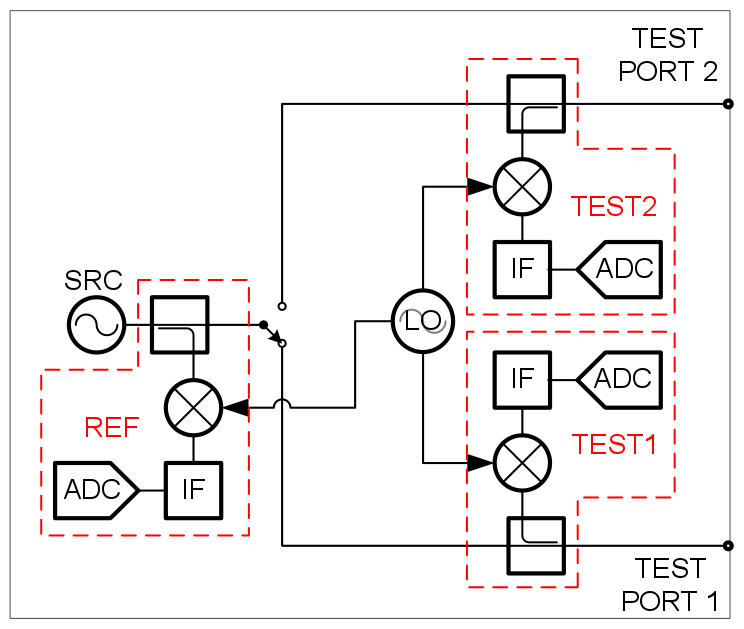
\includegraphics[width=0.4\textwidth]{Pictures/vna}
\caption{Принципиальная схема векторного анализатора.}
\label{fig:vna}
\end{wrapfigure}

На \autoref{fig:vna} изображена упрощенная схема прибора. В векторных анализаторах используется \textit{гетеродинирование} -- понижающее частоту преобразование сигнала -- для того, чтобы было возможно цифровое детектирование аналого-цифровым преобразователем (Analog-to-Digital Converter, ADC). Гетеродинирование происходит в \textit{смесителях} (mixers, $\otimes$) -- нелинейных элементах, позволяющих получать суперпозиции гармоник, поданных на их входы. В каждом смесителе есть два входа: высокой частоты (Radio Frequency, RF) и гетеродинный (Local Oscillator, LO), и один выход -- промежуточной чатоты (Intermediate Frequency, IF). На первый из входов подается соответственно исследуемый сигнал, а на второй -- близкий к нему по частоте и единый для всех синхронизирующий сигнал LO. После прохождения через миксер в блоке обработки промежуточной частоты отфильтровывается сигнал на частоте $|f_{LO} - f_{RF}|$ и, затем, через АЦП направляется в процессор. 

В итоге, схема измерения S-параметров следующая: источник микроволн (SouRCe, SRC) подключается к одному из направлений 1 или 2 в зависимости от измерения $S_{*1}$ или $S_{*2}$; в этот же момент он копируется при помощи \textit{направленного ответвителя} (directional coupler, $\vcenter{\hbox{
\includegraphics[width=0.02\textwidth]{Pictures/coupler}}}$) и направляется в контур сравнения (REFerence, REF), где гетеродинируется; затем либо в блоке TEST1, либо в блоке TEST2 в зависимости от измерения $S_{1*}$ или $S_{2*}$ гетеродинируется сигнал от исследуемой системы. В конечном итоге происходит вычисление процессором конкретного S-параметра на основе собранных АЦП данных по амплитуде и фазе относительно гетеродина. 


\begin{wrapfigure}{r}{0.5\textwidth}
\centering
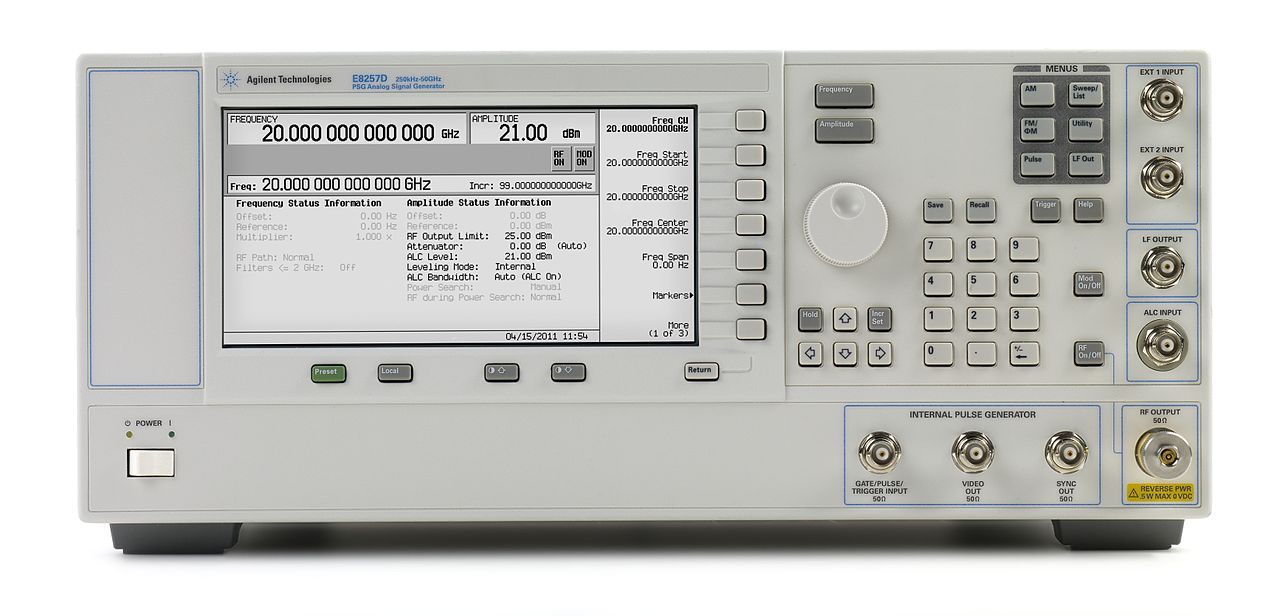
\includegraphics[width=0.4\textwidth]{Pictures/mw_src}
\caption{Источник микроволн Agilent E8257D, используемый в эксперименте.}
\label{fig:mw_src}
\end{wrapfigure}

\paragraph{Аналоговый источник микроволнового излучения.} Для экспериментов с кубитами отдельно требуется просто источник чистого гармонического микроволнового сигнала, позволяющий в широких пределах изменять его частоту, мощность и производить амплитудную и фазовую модуляции. В лаборатории в МИСиС установлены два одинаковых источника модели, изображенной на \autoref{fig:mw_src}. Эти приборы работают в диапазоне 100 МГц -- 20 ГГц и могу быть применены в экспериментах с двухтоновой спектроскопией, с импульсными воздействиями на образец, а также в качестве гетеродина в случае использования смесителей.

\begin{wrapfigure}[18]{r}{0.45\textwidth}
\centering
\begin{subfigure}[t]{0.35\textwidth}
	\centering
	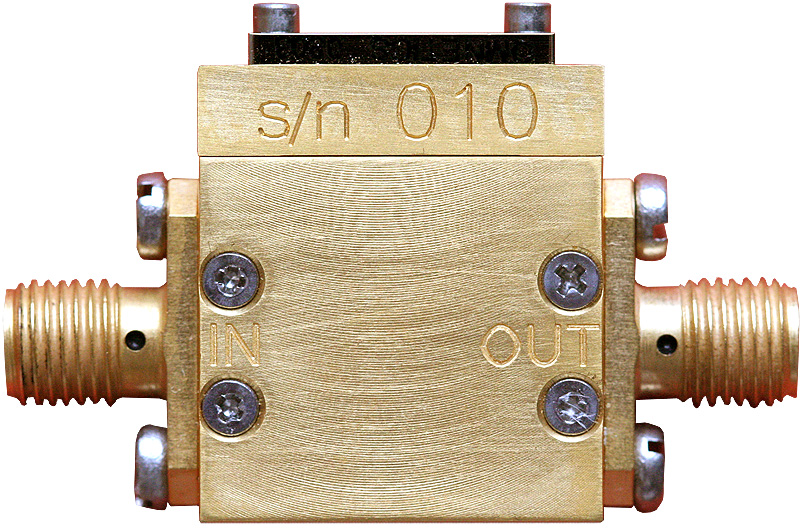
\includegraphics[width=0.8\textwidth]{Pictures/cryoamp}
	\caption{Криогенный усилитель компании Low Noise Factory.}
\end{subfigure}

\begin{subfigure}[t]{0.35\textwidth}
	\centering
	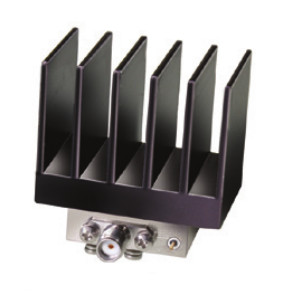
\includegraphics[width=0.6\textwidth]{Pictures/amp}
	\caption{Комнатный усилитель компании Mini Circuits.}
\end{subfigure}
\caption{Использованные усилители.}
\label{fig:amps}
\end{wrapfigure}

\paragraph{Усилители.} Для проведения измерений слабых сигналов, поступающих от образца, требуется их усиление. Для этого в лабораторной установке используются два типа усилителей (\autoref{fig:amps}): комнатные и низкотемпературный малошумящий HEMT-усилитель. Первые работают снаружи криостата, а второй находится внутри него при температуре 4 К. Главными параметрами усилителя являются непосредственно коэффициент усиления (в случае вычисления по мощности он измеряется в dBm), ширина полосы усиления и отношение сигнал/шум. 

\paragraph{Держатель образца.}

 В данной работе использовался созданный в лаборатории широкополосный криогенный держатель образца\cite{averkin2014} (\autoref{fig:sample_holder}). Держатели образцов являются следствием макроскопичности человека, который, в конце концов, должен поместить чип в криостат и подключить его к таким же, как и он сам, макроскопическим приборам. Таким образом, они являются местом, где макро-масштаб переходит в мезо- и микро-масштаб. Связь чипа с образцом производится при помощи \textit{бондера} -- устройства, позволяющего припаивать миллиметровые провода двумя концами к контактам на держателе и к контактным площадкам на чипе. 
 
\begin{figure}[h]
\begingroup
\captionsetup{width = 0.9\textwidth, justification=normal}
\centering
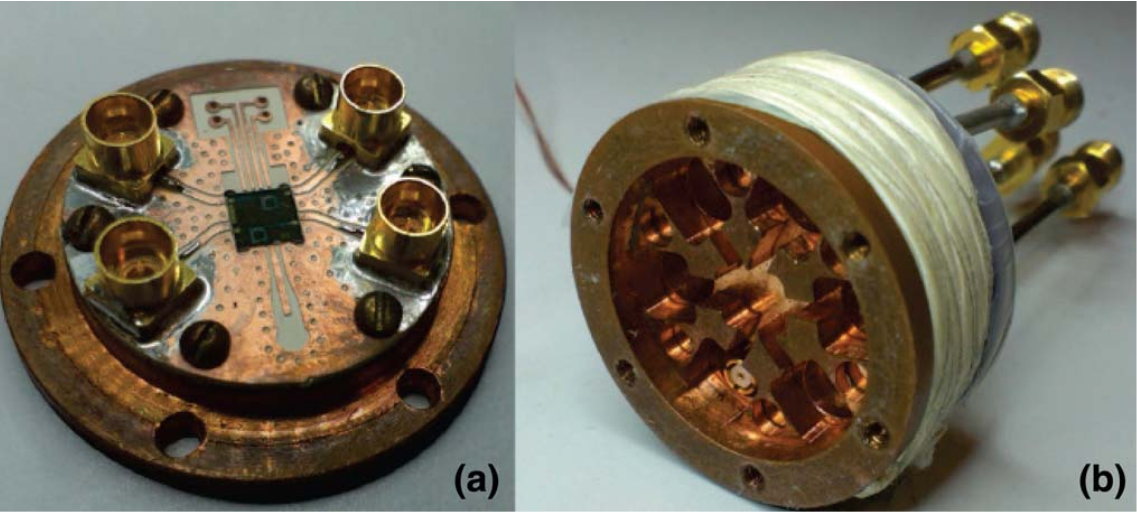
\includegraphics[width=0.75\textwidth]{Pictures/sample_holder}
\caption{Внешний вид держателя\cite{averkin2014} с чипом в нижней части (а). Верхняя часть (b) содержит переходники SMA-SMP и сверхпроводящую обмотку для создания магнитного поля. Разъемы SMP защелкиваются, а не навинчиваются и служат для облегчения установки образца в держатель. Разъемы SMA же стандартны для проводов, приборов и больше по размеру.}
\label{fig:sample_holder}
\endgroup
\end{figure}

Естественно, как любая вынужденная мера, держатель привносит в эксперимент дополнительные помехи. Отличие волнового сопротивления участка с бондами от 50 Ом приводит к отражениям и потерям. Сам держатель требует также специального дизайна и моделирования, так как может резонировать в области интересующих нас частот. Использованный держатель спроектирован с учетом таких особенностей: он минимизирует длину бондов, так как углубление в точности соответствует размеру чипа, имеет плоскую широкую полосу пропускания и резонанс на частоте за пределами области интересов -- это достигается с помощью специальной вставки с вырезами, которую можно видеть на \autoref{fig:sample_holder}~(b).

Однако держатель также позволяет лучше изолировать образец от внешних шумов: для защиты от постоянных магнитных полей на держатель надевается пермаллоевый экран, а также свинцовый сверхпроводящий экран для защиты от переменных полей.


\begin{wrapfigure}{r}{0.45\textwidth}
\centering
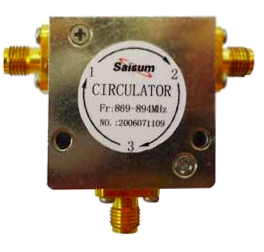
\includegraphics[width=0.3\textwidth]{Pictures/circ}
\caption{Циркулятор. Стрелками показаны направления прохождения сигнала.}
\label{fig:circ}
\end{wrapfigure}

\paragraph{Микроволновые компоненты.} Помимо крупных приборов важны также различные микроволновые устройства, устанавливаемые в линию. Такими, в частности являются аттенюаторы, ослабляющие сигнал (служат для защиты от температурных шумов, подробнее в \autoref{sec:exp_scheme} данной главы) и характеризующиеся коэффициентом ослабления (в dBm), а также полосовые фильтры, снижающие спектральную мощность низкочастотных и высокочастотных шумов. Для тех же целей используются криогенные ферритовые циркуляторы. Циркулятор представлен на \autoref{fig:circ}. В терминах S-параметров циркулятор обладает следующей матрицей рассеяния:
\begin{equation*}
S = \rbrkt{\begin{matrix}
0 & 0 & 1 \\
1 &0 & 0\\
0&1&0
\end{matrix}}
\end{equation*}
Если на один из выходов установить 50-омную заглушку, то циркулятор станет изолятором, пропускающим излучение только в одном направлении.

\subsection{Оборудование постоянного тока}

\begin{wrapfigure}[8]{r}{0.4\textwidth}
\centering
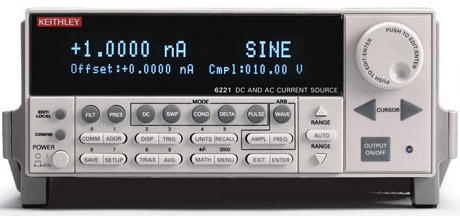
\includegraphics[width=0.3\textwidth]{Pictures/6221}
\caption{Источник тока Keithley 6221.}
\label{fig:6221}
\end{wrapfigure}

\paragraph{Источник постоянного тока.} Для проведения экспериментов с потоковым кубитом (да и вообще практически со всеми современными типами сверхпроводниковых кубитов) требуется подавать на образец постоянное магнитное поле. В эксперименте это реализуется при помощи точного источника постоянного тока и катушки индуктивности, внутри которой находится образец, либо расположенной прямо на чипе спирали. В нашей лаборатории используется источник тока Keithley 6221 (\autoref{fig:6221}), способный выдавать напряжение, обеспечивающее точность протекающего тока до десятков пА, и сверхпроводящий соленоид в 550 витков, намотанный вокруг держателя образца (\autoref{fig:sample_holder}~(b)).


\section{Образец}

В предыдущем разделе было показано, что использовалось в эксперименте для измерения. Теперь настало время поговорить о том, что же все-таки измерялось. Ниже будут обсуждаться общая идея исследовавшегося образца, его компоновка, технология производства образца и характеристики.

\subsection{Схема образца}

Принципиальная схема образца в модели сосредоточенных элементов представлена на \autoref{fig:chip_equiv}. Изначально он создавался\cite{Jerger2013} для \textit{мультиплексирования с разделением по частоте} (frequency-division multiplexing) -- способа одновременно управлять несколькими кубитами, используя только одну передающую линию. Поэтому скомпонован чип следующим образом: непрерывная передающая линия, проходящая через всю кремниевую подложку, емкостно связана с семью четвертьволновыми копланарными резонаторами, обладающими попарно различными резонансными частотами. На конце каждого резонатора, в пучности магнитного поля, находится по кубиту.

\begin{figure}[h]
\centering
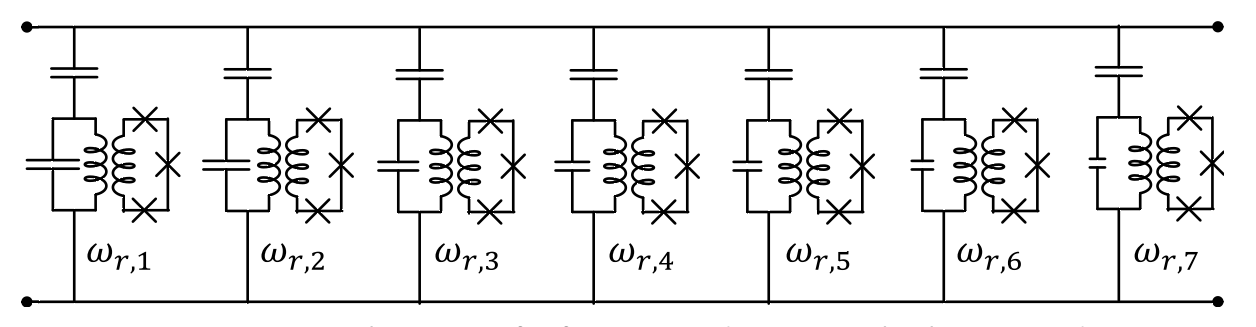
\includegraphics[width=0.9\textwidth]{Pictures/chip_equiv}
\caption{Эквивалентная схема образца\cite{Jerger2013}. $\lambda/4$ резонаторы представлены в модели сосредоточенных элементов.}
\label{fig:chip_equiv}
\end{figure}

\begin{figure}[h]
\begingroup
\captionsetup{width = 0.9\textwidth, justification=normal}

\centering
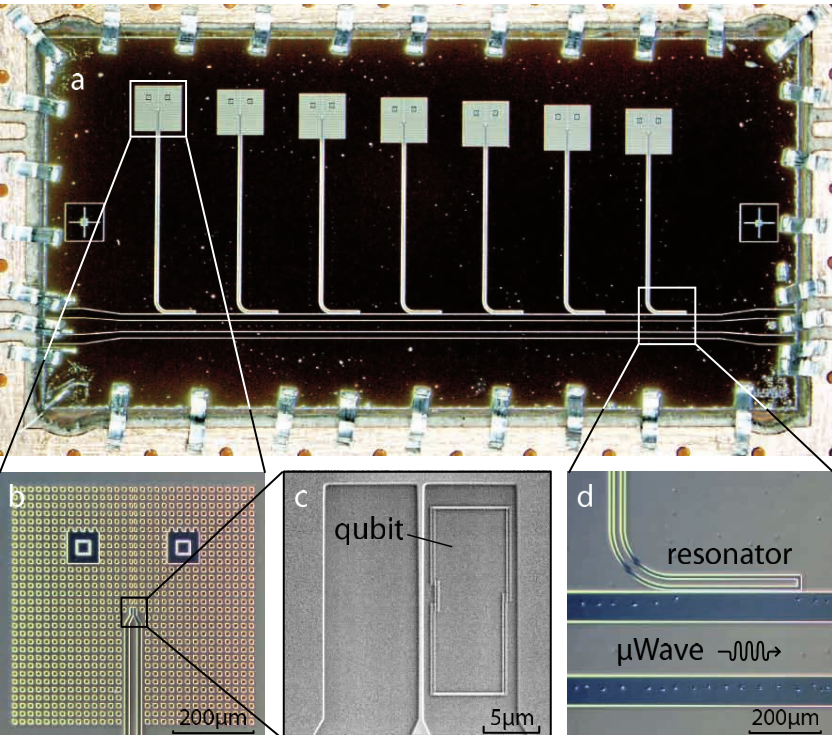
\includegraphics[width=0.8\textwidth]{Pictures/marcus_chip}
\caption{Исследовавшийся образец\cite{Jerger2013}. (a) Общий вид чипа, соединенного ленточными бондами с держателем образца. (b) Замкнутый накоротко конец резонатора, окруженный ловцами вихрей Абрикосова. (c) Кубит, лежащий в резонаторе в области максимальной амплитуды магнитного поля. (d) Резонатор связан с передающей линией через изгиб, образующий конденсатор с ее центральной жилой.}
\label{fig:marcus_chip}
\endgroup
\end{figure}


\subsection{Фабрикация образца}

Изготовление структур на масштабе порядка 1 $\mu$м удобно при совмещении двух технологий: фотолитографии и электронной литографии, так как они позволяют получать одновременно и большие по площади поверхности, например, передающей линии и резонаторов, и мелкие детали -- наноразмерные джозефсоновские переходы. Полученный этими методами образец изображен на \autoref{fig:marcus_chip}.

\paragraph{Фотолитография.} Изготовление структур, больших 1 $\mu$м, возможно при помощи экспонирования фоторезиста электромагнитным излучением видимого диапазона. Процесс в целом разделяется на пять этапов: нанесение фоторезиста, экспонирование, проявление, напыление и удаление лишнего напыленного вещества. Экспонирование может быть либо \textit{масочным}, когда засветка производится через предварительно изготовленную пластину с прорезями, либо \textit{растровым}, когда структура рисуется лазерным лучом. Под действием света резист изменяет свои свойства и позволяет оперировать отдельно или с засвеченной, или с не засвеченной областью. Проявление, в зависимости от типа резиста, удаляет либо засвеченную, либо не засвеченную область фоторезиста. Далее, на открывшуюся после проявки область подложки одним из многих способов напыляется требуемое вещество.
Затем производится удаление оставшегося резиста, вместе с которым уходит также и осажденный на него материал.

\begin{figure}[h]
\centering
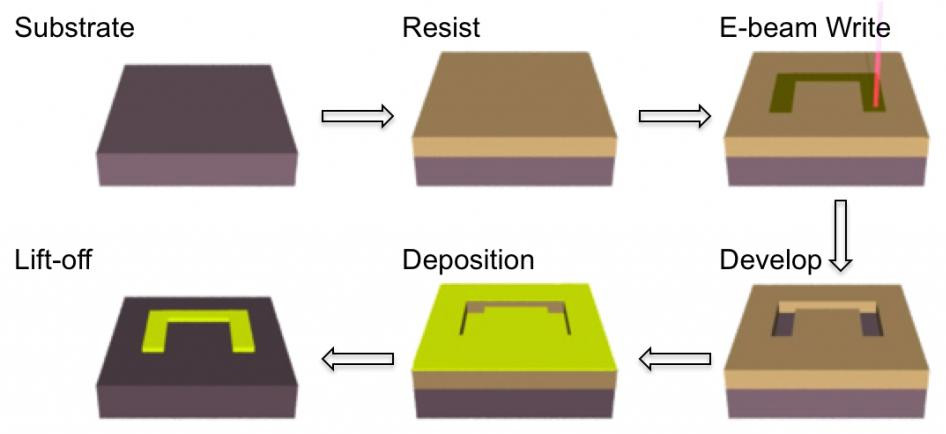
\includegraphics[width=0.6\textwidth]{Pictures/lithography}
\caption{Этапы литографического процесса.}
\label{fig:lithography}
\end{figure}

Фотолитография является наименее ресурсозатратным методом получения наноструктур из существующих на сегодняшний день, и поэтому всегда применяется, если есть такая возможность. Самый простой вид фотолитографии -- это, конечно, масочная фотолитография. Более того, современные масочные фотолитографические методы могут конкурировать с электронной литографией по разрешению. Несмотря на кажущееся дифракционное ограничение, крупные компании, печатающие интегральные микросхемы и использующие фотолитографию в коротковолновом ультрафиолетовом диапазоне ($\approx$190 нм), получают структуры с проектной топологической нормой 14 нм. 

\begin{wrapfigure}[21]{r}{0.5\textwidth}
\centering
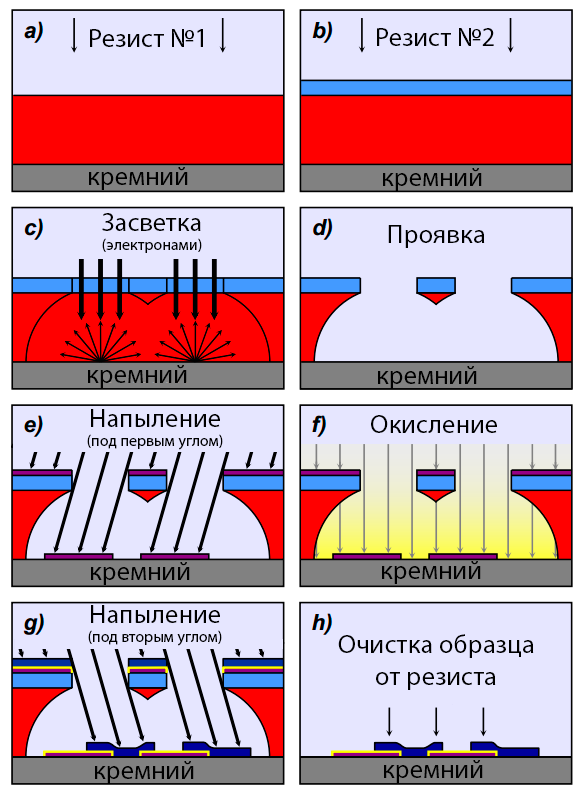
\includegraphics[width=0.45\textwidth]{Pictures/shadow}
\caption{Теневое напыление. G{\"o}ppl M. V.\cite{goppl2009}}
\label{fig:shadow}
\end{wrapfigure}

\paragraph{Электронная литография.} Растровая фотолитография видимого диапазона, которая используется в лабораториях, допускает примерно 500-$\mu$м техпроцесс и применяется для изготовления ``крупных'' элементов (копланарных резонаторов, передающих линий).  Однако для стабильного изготовления маленьких джозефсоновских переходов с размерами около 100 нм применяется электронная литография. Электронный литограф имеет максимальное разрешение порядка 10 нм. Схема электронно-литографического процесса очень похожа на схему, использующуюся в фотолитографии (\autoref{fig:lithography}), однако в связи с тем, что вместо фотонов используются высокоэнергетические электроны, используются другие резисты и соответствующие проявители.

\paragraph{Этап напыления.} Помимо простого напыления, когда, например, металл осаждается на подложку однократно, а затем производится подвзрыв, применяются более сложные техники. Для производства маленьких джозефсоновских переходов используется \textit{теневое напыление} (\autoref{fig:shadow}). Идея этой технологии в том, что при напылении алюминия через маску под двумя разными углами проекции от двух напылений могут накладываться друг на друга. Если перед вторым напылением напустить в камеру кислород, то между двумя слоями алюминия окажется слой Al$_2$O$_3$ -- диэлектрика, и получится необходимый SIS-переход. 
 
\subsection{Соотношение экспериментального объекта с теоретической моделью}

\begin{figure}
\begingroup
\captionsetup{justification=normal}
\centering
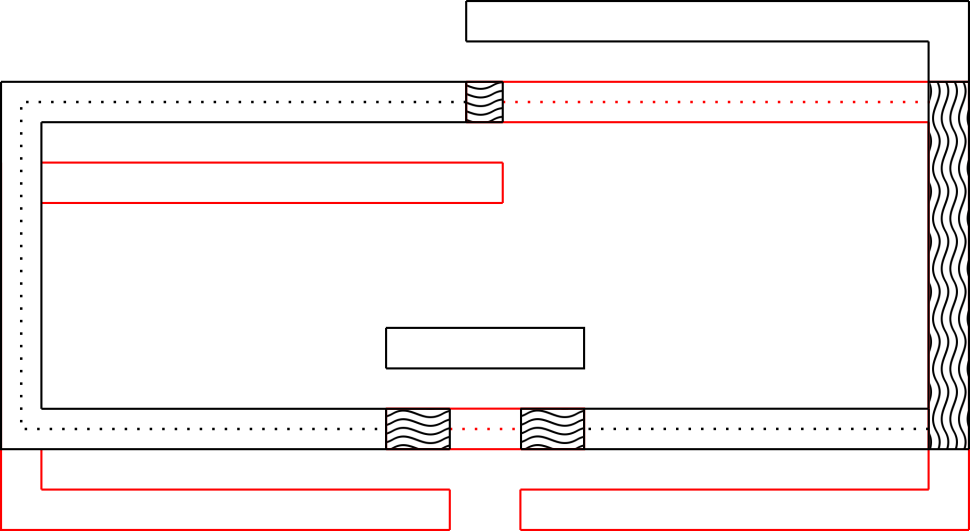
\includegraphics[width=0.7\textwidth]{Pictures/qubit_scheme}
\caption{Устройство реального кубита. Черным цветом обозначен верхний слой алюминия, красным -- нижний, волнистыми линиями выделены получающиеся переходы, а пунктир показывает, как протекает ток (цвет соответствует слою протекания).}
\label{fig:qubit_scheme}
\endgroup
\end{figure}

Исследованный образец имеет определенные особенности, в какой-то степени отличающие его от теоретической модели. Несомненно, есть вопросы касательно многих пунктов: применимость теории Гинзбурга-Ландау, синусоидальность фазо-токового соотношения. Вызывает вопросы применимость основного уравнения эволюции, теории отклика, проблемы квантового измерения и т.д. и т.п. -- это довольно общие темы, присутствующие во всех экспериментах с квантовыми системами, и можно сгинуть, пытаясь выяснить на них ответы.

С другой стороны есть отличия, влияние которых возможно довольно просто увидеть и оценить. Первое состоит в том, что в изготовленном кубите, как видно из \autoref{fig:qubit_scheme}, на самом деле не три джозефсоновских перехода, как в теории, а четыре. Однако один из них столь велик, что разность фаз на нем практически постоянна и примерно равна нулю, поэтому он исключается из рассмотрения в гамильтонине \eqref{eq:hamiltonian} \autoref{chap:theory}. Второе -- одинаковость больших переходов в кубите: так как при фабрикации нельзя с абсолютной точностью создать равные площади элементов, что опять же означает приближенность использованного гамильтониана. Далее, конкретно в этой работе использовался образец с резонатором, не встроенным в линию, а расположенным рядом. Поэтому нужно иметь в виду, что теория отклика требует определенных коррекций, так как в чистом виде она выведена для резонаторов первого типа, у которых на резонансной частоте имеется максимум пропускания, а не минимум, как во втором случае.

Упомянутые вопросы, несмотря на свою простоту, не находят ответа в данной работе. Автор оставляет и себе, и читателю возможность отправиться на поиски ответов, найти их, обработать и выразить в какой-то своей научной работе.


\section{Схема эксперимента}  \label{sec:exp_scheme}

\begin{wrapfigure}[30]{r}{0.5\textwidth}
\begingroup
\captionsetup{justification=normal, width=0.45\textwidth}
\centering
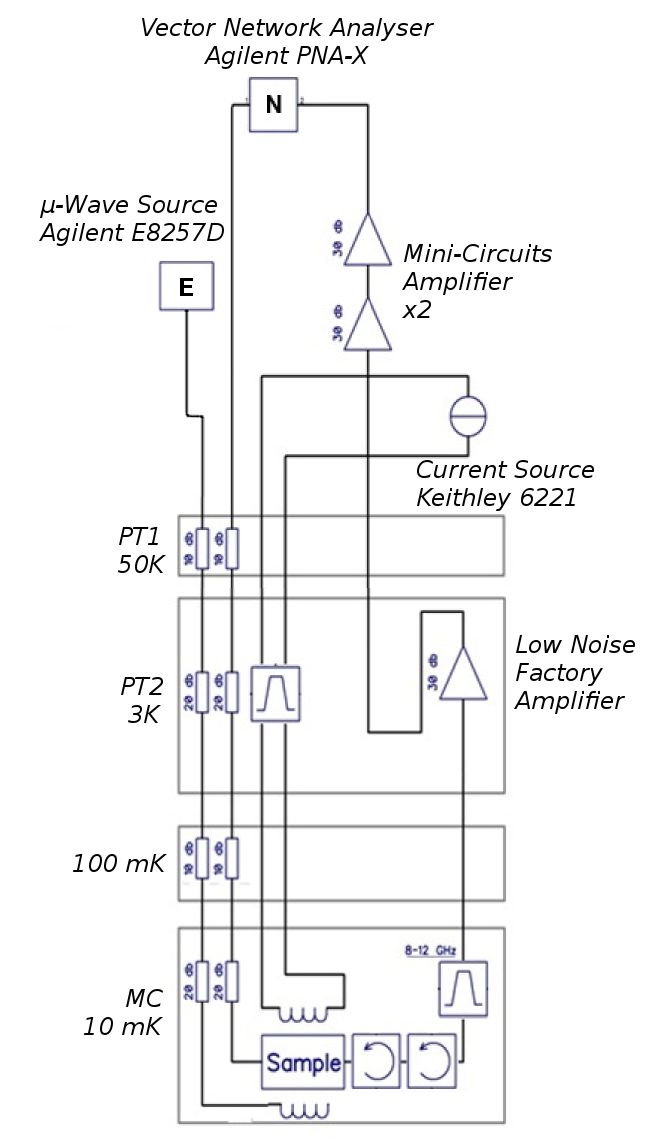
\includegraphics[width=0.5\textwidth]{Pictures/crio_scheme2}
\caption{Схема расположения микроволновых элементов и приборов внутри и снаружи криостата.}
\label{fig:cryo_scheme}
\endgroup
\end{wrapfigure}


В данном разделе будет обсуждаться методика исследования образца. При начале любого эксперимента всегда возникает много мелких и не очень проблем, с которыми так или иначе приходится бороться. Схема установки и порядок проведения эксперимента во многом определяются именно тем, насколько они помогают избежать неудобств.

\subsection{Схема установки}

Схема компоновки элементов и приборов для проведения спектроскопических измерений (для проведения импульсных измерений внутренняя часть будет такой же, а внешняя гораздо сложнее) представлена на \autoref{fig:cryo_scheme}. На нем изображена как и общая уровневая структура криостата, так и проложенные в нем линии коммуникаций. Удобно разделить повествование на две части: сначала обсудим внешнюю, а затем внутреннюю по отношению к криостату части системы.

\paragraph{Внешняя часть.} Как видно из общей схемы, снаружи установлено три прибора (векторный анализатор цепей Agilent PNA-X, источник микроволнового излучения, источник постоянного тока) и два одинаковых комнатных усилителя. Микроволновые сигналы от них передаются к криостату по коаксиальным проводам, где те ввинчиваются в вакуумные SMA-разъемы, а постоянный ток по обычным проводам к коробке, из которой он переходит в медные витые пары одной из трех DC-линий, проложенных в откачиваемой части установки. Снаружи на микроволновые кабели также устанавливаются фильтры постоянного тока, который может создать нежелательные магнитные поля на чипе в силу отсутствия разрывов в микроволновой цепи.

\paragraph{Внутренняя часть.} Внутри криостата постоянный и переменных сигналы предварительно обрабатываются, причем по-разному. Постоянный сигнал просто фильтруется, чтобы как можно больше уменьшить ненужные для нас случайные переменные сигналы, а вот микроволновые линии устроены сложнее. Входной микроволновый сигнал ослабляется аттенюаторами на каждой из пластин рефрижератора. Это необходимо, так как иначе температурный шум попадал бы снаружи криостата внутрь практически не ослабленным, что сводило бы на нет все усилия по охлаждению образца. Так как температура на каждой следующей пластине ниже, чем на предыдущей, на каждой требуется установить по аттенюатору. Далее, сигнал от анализатора приводится в образец, а оный от источника микроволн -- на колечко, создающее таким образом переменное поле. Однако иногда применяется направленный ответвитель, чтобы пустить по одному и тому же кабелю как сигнал от анализатора, так и сигнал от источника с таким же итоговым эффектом.

Выходной микроволновый сигнал сразу же направляется в два последовательно установленных криогенных циркулятора, работающие в режиме изоляции. Это позволяет убрать шумы, приходящие на образец с верхних уровней криостата и снаружи, и в то же время не ослаблять и без того уже очень слабый полезный сигнал. Чуть позже излучение проходит  через криогенный усилитель, являющийся также по сути и полосовым фильтром, и выходит из криостата.

\subsection{Порядок проведения эксперимента}

\paragraph{Детектирование кубита.} Для обнаружения кубита, связанного с резонатором, можно использовать следующую методигу: определив местоположение резонатора по частоте, нужно установить анализатор цепей в минимум прохождения, а затем пройти источником тока по некоторому диапазону значений магнитного поля. В тот момент, когда частота кубита под действием поля совпадет c частотой резонатора, в результате снятия вырождения произойдет расщепление частот поглощения и значительное увеличение пропускания $S_{21}$ на прежней частоте. В результате на графике $S_{21} (I)$ возникнут периодические пики, период которых будет соответствовать изменению потока через кубит на один квант $\Phi_0$ (см. \eqref{eq:hamiltonian} -- гамильтониан периодичен по $\Phi$). Фактически, такая процедура соответствует измерению среза трехмерного графика \autoref{fig:rabi_spec_dyn} в одной точке по оси Oy, соответствующей частоте резонатора.

\paragraph{Однотоновая спектроскопия.} Для получения спектра квазипересечений (как на \autoref{fig:rabi_spec_dyn} \autoref{chap:theory}) достаточно только анализатора цепей и источника тока. Анализатор проходит по выборке частот из заданного диапазона для каждого значения тока, выдаваемого источником, и измеряет коэффициент прохождения $S_{21}$ на каждой из этих частот. В зависимости от магнитного поля, и, следовательно, от тока, уровни системы перестраиваются, и частота поглощения изменяется, что и обнаруживается анализатором.

При измерении спектр стабильного состояния зависит от среднего числа фотонов в резонаторе. Моделирование проводилось для ситуации когда это число меньше единицы, поэтому для согласованности с теорией требуется подавать на резонатор достаточно малую мощность, чтобы диссипация успевала компенсировать накачку даже при малой его заселенности. Для оценки необходимой мощности требуется решить уравнение следующего вида (для простоты здесь берется резонатор без кубита и $T=0$):
\begin{equation}
\frac{\partial}{\partial t} \hat \rho = \frac{i}{\hbar}\sbrkt{\hat \rho, \hbar \omega_r \hat a^\dag \hat a - \hbar B (\hat a^\dag + \hat a) \cos \omega t}  + \kappa \mathcal{D}[a]\hat \rho.
\label{eq:master_osc}
\end{equation}
Запишем его сначала для величины $\left< \hat a \right> = \Tr{\hat \rho \hat a}$. Для этого надо взять след от всего уравнения \eqref{eq:master_osc}, умноженного справа (или слева) на $\hat a$. Далее, переставить производную	по времени, чтобы получить слева от знака равенства $\partial_t \left< \hat a \right>$. Воспользовавшись соотношением $\sbrkt{\hat a, \hat a^\dag} = 1$ и циклическим свойством следа $\Tr{\hat O_1 \hat O_2} = \Tr{\hat O_2 \hat O_1}$, получим итоговое уравнение:
\begin{equation*}
\partial_t \left< \hat a \right> = - i\omega_r \left< \hat a \right> - \frac{\kappa}{2} \left< \hat a \right> + i B \cos \omega t.
\end{equation*}
Стоит отметить, что это уравнение полностью эквивалентно уравнению движения на величину $ a = \sqrt{\frac{m\omega_0}{2\hbar}} \rbrkt{x-i\frac{p}{m\omega_0}} $ для классического осциллятора\cite{thuneberg2013}. Решение для вынужденных колебаний в приближении вращающейся волны:
\begin{equation}
\left< \hat a \right> (t) = \frac{iB/2}{i(\omega_r-\omega) + \kappa/2}e^{-i\omega t} \equiv \frac{B/2}{\omega_r-\omega - i\kappa/2}e^{-i\omega t}.
\label{eq:a_ss}
\end{equation}
Аналогично,
\begin{equation}
\left< \hat a^\dag \right> (t) = \frac{B/2}{\omega_r-\omega + i\kappa/2}e^{i\omega t}.
\label{eq:a+_ss}
\end{equation}
Далее, построим уравнение для величины $\left< \hat n \right> = \left< \hat a^\dag \hat a \right>$:
\begin{equation*}
\partial_t \left< \hat a^\dag \hat a \right> = -\kappa \left< \hat a^\dag \hat a \right> + i B \rbrkt{\left< \hat a^\dag \right>  - \left< \hat a \right> } \cos \omega t.
\end{equation*}
Подставляя в него решения \eqref{eq:a+_ss} и \eqref{eq:a_ss}, полагая $\partial_t \left< \hat n \right>_{ss} = 0$ и применяя RWA, получим окончательно установившееся число фотонов в резонаторе при заданной амплитуде вынуждения:
\begin{equation}
\left< \hat n \right>_{ss} = \frac{B^2}{\kappa^2 + 4(\omega_r - \omega)^2},
\label{eq:photon_resonance}
\end{equation} 
Как видно, число фотонов имеет резонансное поведение, и в случае точного совпадения частоты вынуждения с собственной частотой равно $B^2/\kappa^2$. Следует опять отметить, что полученное выражение \eqref{eq:photon_resonance} совпадает с аналогичным классическим\cite{thuneberg2013}.

Теперь надо понять, как соотнести амплитуду вынуждения с параметрами излучения в передающей линии. Это можно сделать упрощенно без учета импедансов передающих линий справа и слева от резонатора следующим образом. Как видно на схеме \autoref{fig:chip_equiv}, если бы не связывающий конденсатор, то имеел бы место стандартный токовый резонанс. От конденсатора можно избавиться, используя преобразование Нортона. После него связывающая емкость $C_\kappa$ может быть включена в конденсатор резонатора, а уравнение движения будет выглядеть следующим образом: 
$$
(C+C_\kappa) \ddot{\Phi} + \frac{\Phi}{L} = I_{no}(t) = \omega C_\kappa V^0_{tl} \sin(\omega t),
$$
где $I_{no}(t)$ -- нортоновский эквивалентный источник тока, a $C+C_\kappa\approx C$. Амплитуда напряжения в линии равна $V_{tl}^0 = \sqrt{P_{\mu\text{-}wave}Z_0}$. Амплитуда тока эквивалентного источника $I^0_{no}$ соотносится с величиной $В$, стоящей в гамильтониане, следующим образом (см. \eqref{eq:osc_driving_term}): 
$$
B = \frac{I_{no}^0}{\sqrt{2\hbar \sqrt{C/L}}} = \frac{\omega C_\kappa V_{tl}^0} {\sqrt{2\hbar \sqrt{C/L}}},
$$
где $C$ и $L$ -- эквивалентные индуктивность и емкость резонатора, равные примерно 250 фФ и 1 нГн, соответственно\cite{Jerger2013}. 

В итоге, получаем необходимую мощность для заселенности в один фотон (для связывающей емкости в 16 фФ, дающей нагруженную добротность примерно 1000 на частоте 7 ГГц, $\kappa = \omega_r/Q_l$):
$$
P_{\mu\text{-}wave} \approx \frac{2\hbar \sqrt{C/L} \kappa^2}{\omega_r^2 C_\kappa Z_0} = \frac{2\hbar \sqrt{C/L}}{Q_l^2 C_\kappa Z_0}  \approx 10^{-16} \text{Вт}.
$$
Это соответствует ослаблению в dBm:
$$10 \log_{10} \frac{P_{\mu\text{-}wave}}{10^{-3} \text{Вт}} = -130\ dBm.$$
Таким образом, по расчету, к 60 dBm аттенюаторов требуется еще как минимум 70 dBm ослабления на выходе анализатора. 

\paragraph{Двухтоновая спектроскопия.} Этот метод измерения идейно близок к дисперсионному считыванию кубита при помощи резонатора, однако производится без необходимости использования устройств, способных выдавать микроволновые импульсы фиксированной длины.
\begin{figure}[h!]
\captionsetup[subfigure]{justification=normal, width = 0.9\textwidth}
\centering
\begin{subfigure}[b]{0.35\textwidth}
\centering
\includegraphics[width=0.9\textwidth]{Pictures/2tone}
\caption{Упрощенная схема переходов между уровнями (зеленые линии) в резонансном режиме, возникающих при однотоновой (обозначены черными стрелками) и при двухтоновой (цветные стрелки) спектроскопии.}
\end{subfigure}
\begin{subfigure}[b]{0.6\textwidth}
\centering
\includegraphics[width=0.9\textwidth]{Pictures/two_tone}
\caption{Симуляция двухтоновой спектроскопии в дисперсионном режиме. Измеряемая величина -- число фотонов $\langle \hat a^\dag \hat a \rangle$, поглощенное системой после 5 $\mu$с эволюции в зависимости от магнитного поля и частоты второго тона. Видны переходы $\ket{0, g}\rightarrow\ket{0, e}$ (однофотонный и двухфотонный), а также переход $\ket{0, e}\rightarrow\ket{1,g}$. Также видна особенность в числе фотонов в центре (ср. \autoref{fig:rabi_freq_spectrum}).}
\end{subfigure}
\caption{Двухтоновая спектроскопия. На (а) представлена качественная идея эксперимента, а на (b) результат точного численного моделирования.}
\label{fig:2tone}
\end{figure}
Для проведения такого измерения требуется установить анализатор на измерение пропускания только на одной частоте (первый тон), равной частоте резонатора, дисперсионно сдвинутой кубитом в основном состоянии (это всегда получается, так как провал в прохождении в эксперименте находится именно на этой частоте). Далее, дополнительное излучение (второй тон) от микроволнового источника либо подмешивается через направленный ответвитель, либо подается на колечко, висящее над образцом, и когда его частота оказывается близкой к частоте кубита, оно возбуждает в нем затухающие Раби-осцилляции, как на \autoref{fig:bloch} \autoref{chap:theory}. За время возбуждения кубит оказывается в смешанном состоянии по 50\% на состояние, что позволяет наблюдать первым тоном переходы с частотой, дисперсионно сдвинутой как вниз, так и вверх, но с половиной амплитуды, что эффективно приводит к изменению пропускания первого тона. На \autoref{fig:2tone}~(a) приведена упрощенная схема возникающих переходов для системы в резонансном случае. В случае однотонового режима сигнал-наблюдатель обнаруживает пропускание на двух частотах $\omega_r \pm g\sin \theta$ (см. \autoref{fig:rabi_spectrum}~(\subref{fig:rabi_analytic_spectrum})), однако если на момент его включения система с некоторой вероятностью уже была на уровне $\ket{1}$, то возникнут дополнительные переходы, обозначенные синими стрелками, на частотах, ранее не наблюдавшихся -- таким образом, второй тон ``открывает'' переходы на трех дополнительных частотах, но ослабляет переход на прежней частоте.
 
На \autoref{fig:2tone}~(b) приведено моделирование отклика системы на негармоническое возмущение, состоящее из операторов как $\mathcal{\hat V}_q$, так и $\mathcal{\hat V}_r$, осциллирующих на различных частотах от $0.1\,\omega_r$ до $1.2\,\omega_r$ и $\omega_r$ соответственно. Цветовой масштаб отражает число фотонов $\left< \hat a^\dag \hat a \otimes \mathbbm{1}_q \right>$, которое набирает система за 5 $\mu$с. Здесь не применялась теория отклика, однако несмотря на это вид спектра оказывается правильным. В итоге на рисунке виден гиперболический спектр кубита (0.2$\,\omega_r$ в точке минимума), а также второстепенные переходы: двухфотонный кубитный спектр (0.1$\,\omega_r$ в точке минимума) и перевернутый спектр перехода $\ket{0, e}\rightarrow\ket{1,g}$ (0.8$\,\omega_r$ в точке максимума). Чем больше мощность как первого, так и второго тонов, тем больше число наблюдаемых второстепенных переходов, так как большая интенсивность второго тона увеличивает вероятность многофотонных процессов, а первый тон большой мощности обеспечивает ненулевую заселенность уровней резонатора фотонами, которые смогут участвовать в дополнительных многофотонных переходах.


\chapter{Результаты}

\section{Общая характеристика резонаторов с кубитами}

В эксперименте были обнаружены все семь резонаторов. Их параметры отражены в  \autoref{table:res+qubs}. Добротности резонаторов весьма велики, а также на каждом из них была заметна периодичность по магнитному полю -- свидетельство того, что они индуктивно связаны со сверхпроводящим кольцом (не обязательно кубитом), в котором квантуется поток.	

\begin{table}[h]

\begin{tabular}{|l|c|c|c|c|c|c|c|}
\hline
Номер резонатора/кубита & 1 & 2& 3&4&5&6&7 \\
\hline
Частота, ГГц & 10.43 & 10.5 & 10.6 & 10.66 & 10.75 & 10.83 & 10.88 \\
\hline
Добротность & 89 000 & 78 800 & 53 000 & 59 200 & 89 600 & 92 000 & 71 200\\ 
\hline
Период по потоку, мкА & 235 & 211 & 200 & 196 & 186 & 183 & 185\\
\hline
\end{tabular}
\caption{Параметры резонаторов и периодичность кубитов по потоку.}
\label{table:res+qubs}
\end{table}

Периоды были определены по методу, который описывался ранее в \autoref{sec:exp_scheme} \autoref{chap:exp}. Видно, что они уменьшаются от резонатора к резонатору, что говорит о наличии градиента магнитного поля на образце, так как площади всех кубитов были одинаковыми.  Несмотря на то, что периодическая зависимость пропускания от тока наблюдалась в каждом случае, только в трех резонаторах из семи на графиках наблюдались явные пики $S_{21}(I)$, которые должны присутствовать при $\Delta < \omega_r$. 


\begin{figure}
\centering
\begin{subfigure}[t]{0.45\textwidth}
\centering
\includegraphics[width=0.9\textwidth]{Pictures/two-tone_spectrum2}
\caption{Второй резонатор/кубит. Фаза.}
\end{subfigure}%
\begin{subfigure}[t]{0.45\textwidth}
\centering
\includegraphics[width=0.9\textwidth]{Pictures/two-tone_spectrum1}
\caption{Третий резонатор/кубит. Амплитуда.}
\end{subfigure}

\vspace{.5cm}
\begin{subfigure}[t]{0.45\textwidth}
\centering
\includegraphics[width=0.9\textwidth]{Pictures/two-tone_spectrum3}
\caption{Пятый резонатор/кубит.\\ Амплитуда.}
\end{subfigure}%
\begin{subfigure}[t]{0.45\textwidth}
\centering
\includegraphics[width=0.9\textwidth]{Pictures/two-tone_spectrum3_pha}
\caption{Пятый резонатор/кубит. Фаза.}
\end{subfigure}

\caption{Спектры различных кубитов. Спектры (с) и (d) относятся к резонатору и кубиту, которые были использованы в дальнейшем эксперименте. Обозначения ``амплитуда'' и ``фаза'' означают, что цветом обозначены соответственно $|S_{21}|$ или $Arg[S_{21}]$}
\label{fig:two_tone_exp}
\end{figure}


\section{Cпектры кубитов}

\subsection{Двухтоновая спектроскопия малой мощности}
 
Методом двухтоновой спектроскопии, описанном в предыдущей главе, были получены спектры трех из семи кубитов на образце. Остальные четыре либо находились выше резонатора по частоте ($\Delta$ > $\omega_r$), либо вовсе не работали, как кубиты. Результаты измерений представлены на \autoref{fig:two_tone_exp}. Как видно, все три спектра представляют собой комбинацию из горизонтального участка от резонатора и гиперболы от кубита (см. уравнение \eqref{eq:trunc_hamiltonian} \autoref{chap:theory}), причем минимумы у всех трех гипербол находятся на примерно на одной высоте -- около 1 ГГц. 

Изначально предполагалось, что частоты $\Delta$ всех кубитов будут различны, так как эксперименты с аналогичным образцом\cite{Jerger2013} показывали значения от 2 до 6 ГГц. Однако в данном эксперименте у всех кубитов фундаментальные расщепления оказались очень близки и, более того, малы по отношению к $\omega_r$: примерно в 10 раз меньше. Такие параметры не вполне подходили для запланированных экспериментов, так как во-первых, нельзя наблюдать зависимость расщепления в резонансном режиме от $\Delta/\omega_r$ (теория предсказывает сильное уменьшение расщепления при малом значении этого числа при прочих примерно равных параметрах), а также, в силу малости этого отношения, ожидались проблемы с наблюдением квазипересечений (из-за их компактности может не хватить разрешения по току). 

Также следует отметить, что ширина линий спектров на верхних двух рисунков сильно отличается от ширины на нижней, которая достигает порядка 1 ГГц. По ширине линий можно оценить времена жизни кубитов -- для верхних это десятки наносекунд, а для нижнего это около 1 наносекунды. Такие времена жизни считаются весьма малыми и говорят о плохом качестве образца. Уточнить приведенные значения можно с использованием импульсного микроволнового оборудования, наблюдая, например, затухание Раби-осцилляций.

\subsection{Двухтоновая спектроскопия большой мощности} 

Для наблюдения дополнительных переходов и экспериментального изучения структуры уровней исследуемой системы можно подавать большую мощность второго тона, который начнет вызывать, например, двухфотонные и другие подавленные в первом порядке переходы. Результат подобного измерения с пятым резонатором/кубитом можно видеть на \autoref{fig:two-tone_highpower}. 

\begin{figure}
\begingroup
\captionsetup{justification=normal}
\centering
\includegraphics[width=0.8\textwidth]{Pictures/two-tone_spectrum_highpower}
\caption{Спектроскопия большой мощности для пятого резонатора. Линии плохо различимы из-за присутствия паразитных вертикальных откликов -- ``засветки'', возникающей при совпадении частот кубита и резонатора.}
\label{fig:two-tone_highpower}
\endgroup
\end{figure}

На рисунке видно, что линии спектра плохо различимы из-за большого числа паразитных вертикальных откликов: когда кубит оказывается в резонансе с резонатором, возникает сильное уменьшение поглощения вне зависимости от частоты второго тона, что выглядит на графике как вертикальная полоса ``засветки''.

\begin{figure}
\begingroup
\captionsetup{justification=normal}
\centering
\includegraphics[width=0.8\textwidth]{Pictures/two-tone_spectrum_highpower_nb}
\caption{Продолжение \autoref{fig:two-tone_highpower} c вычитанием фона. Линии видны лучше, можно видеть одно- и двухфотонную гиперболические линии поглощения кубита (1.5 и 0.75 ГГц при $\Phi=\Phi_0/2$), переход $\ket{0, 0, e}\rightarrow\ket{1, 0, g}$ (9 ГГц при $\Phi=\Phi_0/2$, перевернутая гипербола), а также двухфотонный переход $\ket{0, 0, g}\rightarrow\ket{1,1,e}$ (9 ГГц при $\Phi=\Phi_0/2$).}
\label{fig:two-tone_highpower_nb}
\endgroup
\end{figure}

Уменьшить этот эффект можно через вычитание фона по направлению токов: из каждого ряда данных по току вычитается фиксированный ряд, соответствующей какой-то частоте второго тона. Такая операция зануляет не зависящие от частоты второго тона артефакты, в частности, вертикальные полосы. На \autoref{fig:two-tone_highpower_nb} с вычтенным фоном (вычитался второй ряд данных снизу) лучше различимы линии поглощения второго тона. Присутствуют одно- и двухфотонная гиперболические линии поглощения кубита с минимумами на частотах около 1.5 ГГц и 0.75 ГГц (ср. с \autoref{fig:2tone}~(b)). Также видны горизонтальная линия поглощения самого резонатора на 10.5 ГГц и еще одна горизонтальная линия на 5.9 ГГц -- паразитный резонанс держателя образца. Наличие паразитного резонанса объясняет появление двухфотонного перехода на 8.9 ГГц: переход с основного состояния в состояние, где в резонаторах по одному фотону, а кубит на верхнем уровне, имеет как раз частоту около 18 ГГц. Строгое обоснование возможности такого многофотонного перехода может быть получено в результате численного моделирования композитной системы, однако для получения полного трехмерного графика потребуется много времени, так как при большой мощности возмущения матрица плотности должна иметь большую размерность.


\section{Квазипересечения частот поглощения}

Основной целью работы было исследование спектра квазипересечений на предмет соответствия с теорией, изложенной в \autoref{subsec:rabi_specrum} и \autoref{subsec:rabi_specrum_dyn} \autoref{chap:theory}, и результатами численного моделирования, проведенного на ее основе. Как уже говорилось ранее, планировалось определить, применимо ли приближение вращающейся волны и присутствует ли смещение Блоха-Сиджерта в какой-либо системе на исследуемом образце. Также ожидалось проверить зависимость величины расщеплений Раби от щели кубита, а также от $\sqrt{n+1}$ (см. \autoref{fig:rabi_spectrum}~(\subref{fig:rabi_analytic_spectrum})), где n -- число фотонов в резонаторе\cite{bishop2009}.

В предыдущем разделе указывалось, что из-за малого отношения частот кубитов к частотам их резонаторов ожидаются проблемы в наблюдении квазипересечений. Действительно, так и произошло -- из трех кубитов, измеренных двухтоновой спектроскопией заметной величины квазипересечение дал только один -- пятый, так как был связан с резонатором гораздо сильнее (оценка силы связи может быть произведена опять же по ширине линий двухтоновой спектроскопии). Результаты этого измерения вместе с численным моделированием, использовавшим уравнение \eqref{eq:master_equation} представлены \autoref{fig:anticrossing} и \autoref{fig:anticrossing_vanishing}.


\begin{figure}[h]
\begingroup
\captionsetup[subfigure]{justification=normal, width=0.9\textwidth}
\centering
\begin{subfigure}[t]{0.49\textwidth}
\centering
\includegraphics[height=0.24\textheight]{Pictures/anticrossing_double1}
\caption{Теоретический график. Провал в пропускании следует за предсказанием стационарной модели.}
\end{subfigure}
%
\begin{subfigure}[t]{0.49\textwidth}
\centering
\includegraphics[height=0.24\textheight]{Pictures/anticrossing_double2}
\caption{Экспериментальный график. Средний пик отсутствует, вся верхняя ветвь слишком узкая и слишком низко. Нижняя ветвь совпадает лучше.}
\end{subfigure}
\caption{Теория и эксперимент. Прерывистая линия показывает предсказание стационарного уравнение Шредингера, чтобы облегчить сравнение.}
\label{fig:anticrossing}
\endgroup
\end{figure}


Для построения теоретического графика использовались следующие параметры: $\kappa = 6.5\cdot 10^{-4}$, $\gamma = 0.01,\ \gamma_\phi = 0.007,\ \Delta = 0.2\,\omega_r,\ g=0.03\,\omega_r$. Из величины $g$ заключаем, что система находится в режиме сильной связи. Несмотря на то, что приведенные параметры дают одно из лучших приближений к эксперименту, все равно есть некоторые отклонения. Как видно, экспериментальный график не следует за стационарным решением, частоты поглощения не попадают на расстояния между уровнями. В его центре, где должна наблюдаться особенность, поглощение вовсе пропадает. Подобный эффект может быть вызван либо очень сильной диссипацией на низких частотах (так как тогда перестает быть применим весь формализм с основным уравнением и неизвестно, что может происходить) или наличием температурных шумов в области 1-2 ГГц (моделирование проводилось при T=0 и не учитывало процессов термального возбуждения). Полного соответствия эффектов в теоретической модели и эффектов полученных в эксперименте на \autoref{fig:anticrossing}~(b) не наблюдается, хотя качественное соответствие имеется. Возникает вопрос, измерялся ли действительно кубит, или же это был все же классический, некогерентный оъект, имеющий определенную нелинейность по полю и мощности.

\begin{figure}[h!]
\begingroup
\captionsetup{justification=normal}
\captionsetup[subfigure]{justification=normal, width=0.9\textwidth}

\centering
\begin{subfigure}[t]{0.49\textwidth}
\centering
\includegraphics[width=\textwidth]{Pictures/anticrossing_vanishing}
\caption{Теоретический график. Параметры такие же, как в \autoref{fig:anticrossing}, за исключением $\gamma = \gamma_\phi = 0.1$. Даже при такой диссипации график по-прежнему следует за стационарным решением}
\end{subfigure}
%
\begin{subfigure}[t]{0.49\textwidth}
\centering
\includegraphics[width=\textwidth]{Pictures/anticrossing_vanishing_exp}
\caption{Экспериментальный график. Видно, что правая ветвь намного ярче, чем предсказывается теорией, а так же расположена выше прерывистой линии.}
\end{subfigure}
\caption{Теоретические и экспериментальные данные для ненаблюдаемости квазипересечений. Прерывистая линия показывает предсказание стационарного уравнение Шредингера, чтобы облегчить сравнение.}
\label{fig:anticrossing_vanishing}
\endgroup
\end{figure}


В процессе проведения эксперимента по обнаружению нелинейности расщепления Раби по числу фотонов в резонаторе возник интересный эффект. Хотя такие эксперименты успешно проводились ранее\cite{bishop2009}, в исследованном образце при приближении к области снятия вырождения поглощение пропадало: двух близких частот поглощения нельзя было наблюдать. Это явление можно частично объяснить сильной диссипацией кубита. Когда мы приближаемся к резонансу, добротность системы оказывается равна среднему арифметическому добротностей кубита и резонатора\cite{Blais2004}: в итоге, получаем что изначально узкий пик резонатора оказывается сильно уширен из-за присутствия маложивущего кубита на той же частоте, время жизни которого почти в $\gamma/\kappa$ = 1000 раз меньше, чем у фотона в резонаторе (\autoref{fig:anticrossing_vanishing}). Однако и здесь есть некоторое несоответствие: теория предсказывает сильное ослабление поглощения на всей центральной ветви, чего не наблюдается в эксперименте. Впрочем, для такого сильного затухания основное уравнение может быть уже неприменимо.

\section{Интерференция Ландау-Зинера}

В этом разделе описан эффект, который можно получить, если измерять пропускание на частоте резонатора в зависимости как от магнитного поля, так и от мощности. На \autoref{fig:lzi} представлен результат такого измерения. На рисунке видно, что с увеличением мощности, и, следовательно, заселенности резонатора, возникают сначала отдельные дополнительные эквидстантные пики в пропускании, а затем начинаются странные осцилляции пропускания, наклонные линии и тому подобные эффекты.  Подобный эффект для одиночного кубита, вынуждаемого оператором $\mathcal{\hat V}_q$\cite{oliver2009} называется \textit{интерференцией Ландау-Зинера}, откуда и происходит название раздела.

\begin{figure}[h]
\centering
\includegraphics[width=0.7\textwidth]{Pictures/LZI}
\caption{Своеобразная зависимость от поля и мощности пропускания $S_{21}$ на частоте резонатора.}
\label{fig:lzi}
\end{figure}

Начальные дополнительные пики можно относительно просто объяснить: с увеличением мощности в нерезонансном случае резонатор может поглощать гораздо больше фотонов своей частоты, нежели чем в резонансном случае (стоит только вспомнить картину уровней энергии для обоих режимов, чтобы это понять, \autoref{fig:JCM_MF}). 
Причем для частот кубита, равных удвоенной, утроенной и т.д. частотам резонатора, число фотонов, которые могут быть поглощены на собственной частоте в резонансном режиме становится больше на какое-то число фотонов, чем в режиме $\omega_q = \omega_r$ (так как вырождение снимается как минимум с уровней $\ket{0, \uparrow}$ и $\ket{n, \downarrow}$, которые уже находятся на высоте $n$, однако, как видно на \autoref{fig:JCM_MF}, расщепление на высоте $n$
\begin{wrapfigure}{r}{0.5\textwidth}
\begingroup
\captionsetup{justification=normal, width=0.45\textwidth}
\includegraphics[width=0.45\textwidth]{Pictures/JCM_MF}
\caption{Структура уровней для большого диапазона значений $\varepsilon$. Стрелками обозначены переходы, происходящие под действием возмущения на частоте резонатора.}
\label{fig:JCM_MF}
\endgroup
\end{wrapfigure}
 гораздо слабее, чем в режиме $\omega_q = \omega_r$, но растет с $n$, поэтому эффективно число фотонов, которое успевает поглотиться, оказывается больше). 
Таким образом, при доведении кубита магнитным полем до частот, кратных частотам резонатора, мы получаем расщепление, которое можно обнаружить только при большой заселенности резонатора (при малой заселенности не будет видно разницы в $|\langle \hat a \rangle|$ между случаем резонанса и его отсутствия). Из гиперболичности спектра кубита новые пики должны быть эквидистантными, а затем, по мере отклонения спектра от гиперболы, терять это свойство, что и наблюдалось. 

Остальные описанные эффекты в данной работе не объяснялись, так как требуют точного рассмотрения, которое выходит за рамки данной работы. Можно отметить, что наблюдение подобных эффектов в численном эксперименте потребует учета многофотонных состояний резонатора и работы с матрицей плотности большой размерности, что затрудняет расчет.

\chapter{Заключение}

\section{Список результатов}
В данном разделе приведен перечень основных результатов работы.
\begin{enumerate}

\item Проведено численное моделирование широкого класса эффектов, связанных со стационарным и динамическим поведением исследуемой системы, в силу отсутствия аналитического решения возникающих уравнений. Численные модели послужили для последующей проверки согласования экспериментальных данных с теоретическими.

\item Методом двухтоновой спектроскопии получены спектры потоковых кубитов. По ширине линий спектров оценены времена жизни кубитов. Экспериментально изучена структура уровней исследуемой системы кубит-резонатор при проведении двухтоновой спектроскопии высокой мощности. Обнаружена возможность участия паразитной резонансной моды держателя в динамике системы.

\item Подробно исследована область квазипересечений линий спектров кубита и резонатора. Проведено сравнение с результатами выполненного численного моделирования на основе основного уравнения эволюции для системы.  Обнаруженные различия могут быть объяснены либо сильной диссипацией в использованном кубите на низких частотах, либо наличием низкочастотных температурных шумов.

\item Проведены наблюдения нелинейных по мощности эффектов в поведении зависимости пропускания на частоте резонатора  от тока. Обнаружены дополнительные пики пропускания в точках потока, где частота кубита кратна частоте резонатора, возникающие при большей мощности, чем в обычном резонансном режиме. Этот результат согласуется с теорией.

\end{enumerate}

\section{Итоги работы и планы на будущее}

\hypersetup{hidelinks=false, colorlinks=true}

В заключение хочется сказать, что в ходе работы было проведено множество исследований использованной системы, как численных, теоретических, так и экспериментальных. Теоретическая часть работы, является, вероятно, первым в русскоязычной литературе комплексным обзором по теме сверхпроводящих потоковых кубитов, связанных с микроволновыми резонаторами, подкрепленным строгим и полным численным анализом. Обзор содержит большое количество оригинальных графиков, построенных автором по данным, полученных им непосредственно в процессе численного моделирования. Численные эксперименты (ссылка на репозиторий с исходным кодом использованных программ: \href{https://github.com/vdrhtc/Thesis-simulations}{https://github.com/vdrhtc/Thesis-simulations}) проводились с использованием языка Python и его стандартных научных бибилиотек Numpy, Scipy и Matplolib (решение стационарных уравнений Шредингера), а также специализированной библиотеки для численного анализа квантовых систем: Quantum Toolbox in Python, QuTiP\cite{Johansson2013} (решение нестационарного уравнения Шредингера, основного уравнения эволюции). Экспериментальные данные сопоставлялись с моделированием, в результате чего удалось обнаружить отклонения поведения исследованного образца от общепринятой модели. Также, с использованием теоретических предпосылок, автор сумел объяснить несколько эффектов, ранее подробно не обсуждавшихся -- например, ненаблюдаемость квазипересечений частот поглощения в пределе малого времени жизни кубита и при малом отношении $\Delta/\omega_r$.

В работе анализировались исключительно спектроскопические характеристики образца, но в дальнейшем планируется расширение экспериментов c использованием недавно полученного оборудования для проведения импульсных измерений.

\begin{figure}[h]
\centering
\begin{subfigure}[t]{0.45\textwidth}
\includegraphics[width=0.9\textwidth]{Pictures/new_qubit}
\caption{Снимок с СЭМ первого изготовленного в России кубита.}
\end{subfigure}
\begin{subfigure}[t]{0.5\textwidth}
\includegraphics[width=0.9\textwidth]{Pictures/new_spectrum}
\caption{Экспериментально полученный спектр кубита. Фаза.}
\end{subfigure}
\caption{Первый отечественный кубит. Источник: МЦФИ МФТИ}
\end{figure}

Также в мае 2015 года был получен первый работающий образец с кубитами, изготовленный целиком на производственных мощностях отечественных лабораторий Московского Физико-Технического Университета и Российского Квантового Центра в Черноголовке. Это сулит широкие возможности в дальнейших экспериментах -- обладая технологией для изготовления образцов, можно гораздо быстрее проводить эксперименты, совмещая и фабрикацию, и измерение в одном научно-исследовательском институте (до этого времени образцы изготовлялись в иностранных лабораториях, а измерялись в России). В качестве примера направления дальнейшей работы можно привести цепочки кубитов, расположенных в линии, сверхпроводящие метаматериалы и импульсное их измерение.

\section{Благодарности}

Также в заключение выражаю глубокую благодарность за помощь в работе моему научному руководителю Рязанову Валерию Владимировичу (ИФТТ), а также моему, можно сказать, второму научному руководителю, Шульге Кириллу Владимировичу (МФТИ, МИСиС), который проводил со мной много времени в обсуждениях различных идей, учил проведению измерений и всегда готов был выслушать и дать совет как по теории, так и по эксперименту; Абрамову Николаю Николаевичу (МИСиС), также помогавшему мне в работе со всевозможными приборами, железом, программным обеспечением; всем сотрудникам Лаборатории искусственных квантовых систем МФТИ, которые организовывали научные семинары, в которых я принимал участие и имел возможность обсудить свои мысли и вопросы, а также узнать что-то новое для себя.

\hypersetup{hidelinks=true}
\fi

\bibliographystyle{ugost2008}
\bibliography{Thesis}

\end{document}